\documentclass[12pt,a4paper,leqno]{report}

\usepackage[ansinew]{inputenc}
\usepackage[T1]{fontenc}
\usepackage[english]{babel}
\usepackage{amsthm}
\usepackage{amsfonts}         
\usepackage{amsmath}
\usepackage{amssymb}
\usepackage{chemformula}
\usepackage{siunitx}
\usepackage{braket}
\usepackage{hyperref}
\usepackage{mathtools}
\usepackage{url}
\usepackage{placeins}
\usepackage[toc,page]{appendix}

\let\Oldsection\section
\renewcommand{\section}{\FloatBarrier\Oldsection}

\let\Oldsubsection\subsection
\renewcommand{\subsection}{\FloatBarrier\Oldsubsection}

\let\Oldsubsubsection\subsubsection
\renewcommand{\subsubsection}{\FloatBarrier\Oldsubsubsection}




\pagestyle{plain}
\setcounter{page}{1}
\addtolength{\hoffset}{-1.15cm}
\addtolength{\textwidth}{2.3cm}
\addtolength{\voffset}{0.45cm}
\addtolength{\textheight}{-0.9cm}

\title{The Chemical Path of Eroded Field Soil From Field to Bottom Sediment with Fe K-edge X-Ray Absorption Near Edge Spectroscopy.}
\author{Antti-Jussi Kallio}
\date{}

\begin{document}

\section*{Acknowledgements}
This work was done in the X-ray laboratory of University of Helsinki. I would like to thank my thesis advisor Professor Simo Huotari, who offered his experienced views during the project and made the project possible in the first place. The door to Prof. Huotari's office was always open when I run into trouble spot, or had a question regarding my research. Also our co-workers from Finnish Environment institute, Petri Ekholm and Jouni Lehtoranta, deserve a special acknowledgement for their hard work in preparing the soils and carrying out the incubations, and also for their valuable feedback. Without their passionate participation and input, the project could not have been successfully conducted. 

   I would like to thank Finnish Cultural Foundation for their funding for the Shared Waters project, which this work was part of. One of my co-workers at X-ray laboratory deserves a special gratitude. Ari-Pekka Honkanen offered training for the use of the measurement equipment and gave valuable tips for data analysis. His help allowed this work to reach new heights. For the inspiring working atmosphere i would like to thank all the members of the X-ray laboratory.
   
   Finally I must offer my profound gratitude to my girlfriend Piia and my little boy Touko for providing me their unfailing support and continuous encouragement throughout my studies and through the process of this work. This accomplishment would not have been possible without them. Thank you.
\\ 
\\  
Author
\\
\\
Antti-Jussi Kallio

\newpage     
\tableofcontents   

\chapter{Eutrophication of the Baltic Sea and Erosion of Field Soil}\label{johd}
%
The state of Baltic sea has changed greatly during the past century. Baltic sea is connected to the Atlantic ocean via narrow Danish straits. This means that the water body of the Baltic sea is partly isolated and thus greatly affected by man made pollutions and nutrients. Eutrophication is one of the greatest challenges affecting the ecosystem and the population living around the Baltic sea. Poisonous blue green algal are a sign of eutrophication, and large algal covers are common, as seen in figure \ref{fig:sinileva}. In the bottom of the Baltic sea large areas are anoxic, which along the nutrients accelerate eutrophication.

The main nutrients causing eutrophication are phosphorus and nitrogen. Fertilizers used in agriculture, waste waters and fallout from the atmosphere are the main sources of nutrients. Eutrophication causes increase in algae production, changes in the biocoenosis and in fish population, and also increase of hypoxic bottom waters. It is also tricky to control the eutrophication, since nutrients stored in bottom sediments can be released back to the water, even if nutrient load is decreased.

\begin{figure}[h!]
   \centering
      
\includegraphics[width=\textwidth]{../Kuvat/sinileva.png}
   \caption{Large blue green algae areas on the coast of Finland in July 2018 \cite{ymparisto}.}
   \label{fig:sinileva}
\end{figure} 

The main source of nutrients is agriculture. Two thirds of phosphorus release and over half of the nitrogen is coming from the agriculture \cite{helcom}. In our work we are focusing on phosphorus release coupled to iron cycling in the bottom sediments. The phosphorus can be carried to the sea either by dissolving into the runoff waters, or by engaged in eroded soil, which is also carried by runoff waters. The eroded soil will at some point end in the bottom sediment of the sea, and face anoxic conditions. Iron chemistry is closely related to phosphorus release in sediments. Iron oxides and \ch{SO4} are common electron acceptors in sediments, and the cycling of \ch{C}, \ch{Fe} and \ch{S} is affecting the fate of \ch{P}. \ch{P} can be buried into the sediment, or released into the water in the cycling process. 

We will study the evolution of the chemical state of \ch{Fe} from the field to the water, and ultimately to bottom sediment and anoxic environment. In order to study the chemistry, we are using X-ray absorption spectroscopy, particularly the X-ray absorption near edge spectroscopy, XANES. This element specific technique is sensitive to the chemical state of the element of interest. We will also develop a measurement method to study the mix of sediment and sea water, which is also possible to be used in anaerobic sample preparation. In addition we'll compare the measurements with known reference samples, for example \ch{FeS} and \ch{Fe} oxides, and with the knowledge of sediment \ch{Fe} chemistry try to estimate how the ability of the sediment to bind \ch{P} to \ch{Fe} changes when conditions turn from oxic to anoxic state.

If our measurement technique turns out to be usable, and we are also able to obtain meaningful results, our technique can be used to study larger set of samples and also redox-chemistry of other elements in the soils. With further studies one can form a better picture of the sediment processes, and their effect on eutrophication. This knowledge can be used to form new guidelines for farmers on erosion and phosphorus control measures. Our results can also be applied to other water bodies, affected by eutrophication, not just the Baltic sea.

This work is done with co-operation of Finnish Environment Institute and Physics Department of University of Helsinki, and is part of a large The Shared Waters project financed by the Finnish Cultural Foundation \cite{samassa}.       

\chapter{Phosphorus in Iron Cycling in the Aquatic System }\label{phosphorus}


\section{Soil as a Carrier of Iron and Phosphorus}\label{Soil}
The release of soil, \ch{Fe} and \ch{P} from the fields or from other terrestrial sites and their transport to the aquatic system is a well known and defined process. Iron contributes 5.1 mass percent of the earth's crust \cite{IronSpeciation} and is a major component of many soil-forming parent materials. The concentration of \ch{Fe} in surface soil is on average $3.5\%$ \cite{FeConcentration}, and the concentration is a function of soil characteristics. In Finland the concentration varies between $1.6-7.1\%$ in post-glacier soils \cite{SoilErosion}. On the other hand the more weathered soils for example in Guadalquivir Valley in Spain the \ch{Fe} concentration is measured as low as $0.9\%$ \cite{SoilErosion}. The concentration of \ch{Fe} in eroded soil thus reflects the concentration of the parent soil, though the concentration might be modified by selective erosion, for instance, of fine particles. Half of the \ch{Fe} in riverine particles consists of largely inert \ch{Fe} silicates, and the other half is possibly reducible forms like oxides.

For the sake of simplicity we will call the oxides, hydroxides and oxide-hydroxides of \ch{Fe}(III) as \ch{Fe} oxides. These oxides are common all around the environment, with varying concentrations between one to several hundred $\si{\gram\per\kilo\gram}$ in aerobic soils \cite{FeOxides}. They also exist in variable forms, with different mineralogy, crystallinity, grain size, etc, which affects the the availability and chemical reactivity of the \ch{Fe} oxides. The age of the soil also affects the available \ch{Fe} oxides. For example in warmer and dryer climates with older soils, the \ch{Fe} oxides are often present in crystalline form. On the other hand in boreal conditions the \ch{Fe} oxides are often in poorly crystalline form. The poorly crystalline forms have high capacity to adsorb \ch{P} in neutral pH. \ch{Fe} oxides can also be bound by organic \ch{C}, which can carry the \ch{Fe} to aquatic system \cite{SoilErosion}. 

Both \ch{Fe} and \ch{P} are naturally present in soils, but the use of chemical fertilizers have increased the reserves of \ch{P}. The increase of \ch{P} reserves has been made possible by the high ability of \ch{Fe} and \ch{Al} to capture \ch{P} by ligand exchange reactions \cite{LigandExchange}. The \ch{P} rich surface soil is extracted in erosion processes and transported to water bodies. \ch{P} is released in the aquatic system due to changes in ionic composition. 

Rivers transport $13-\SI{19}{\peta\gram}$ of suspended solids to the oceans per year \cite{IronFlux}. Most of the solids settle out to become sediments in estuary and coastal regions. Total yearly flux of \ch{Fe} is $\SI{960}{\tera\gram}$  and \ch{Fe} oxides is $270-\SI{430}{ \tera\gram}$, mainly as small particles which mostly settle in coastal waters. \cite{SoilErosion}. \ch{P} flux is estimated to be $18-\SI{30}{\tera\gram}$ yearly, of which 25-45\% is expected to be reactive \cite{SoilErosion}.  

Particulate \ch{P} erosion is affected by tillage depth, intensity of tillage, plant cover, soil texture, soil quality, slope and hydrology. The amount of \ch{P} losses are thus highly variable and the type of arable land is the main variable. Particulate \ch{P} is often dominant in runoff from fine-textured soils without permanent plant cover. In The Nordic countries up to 93\% of total \ch{P} is in particulate form in agricultural runoff \cite{Agriculture}. The algae need \ch{P} in a dissolved orthophosphate form, so \ch{P} needs to be released from particles. Algae studies have shown that in eroding river banks only less than $1-13\%$ of \ch{P} and in lake banks no \ch{P} was available \cite{Ellis1988, YOUNG1985434}. On the other hand in agricultural rivers the availability of particulate \ch{P} ranges from 5 to 41\% with norm somewhere between $20-30\%$  \cite{SoilErosion}.

With the previous calculations the current erosion control measures seem appropriate. However they do not take into account any sediment processes, which are the main focus in our research.                        
% Lannoittamisesta

% Jokien kuljetuksesta

% fosfori h�vi�t pelloilta

% 

\section{Role of Sediment}\label{Sediment}
The existing literature on \ch{P} cycling focuses on the link between soil erosion and \ch{P} transport, or \ch{P} bioavailability. However at some point the particles have become part of the sediment and eventually they will face anoxic environment, which has an impact on \ch{Fe} cycling, and thus also affect the fate of \ch{P}.

The sediments reduce \ch{Fe} oxides via two distinct processes \cite{SoilErosion}. The first one is called microbial dissimilatory \ch{Fe} reduction, where the microbes use the oxides as terminal electron acceptors in respiration. In the other process the oxides are reduced chemically by \ch{H2S} formed in microbial \ch{SO4} reduction. For both of these methods the primary energy source for reduction is organic \ch{C}. The flux of organic \ch{C} to the bottom surface decides the dominant mode of reduction. In case of low \ch{C} flux the sediment has plenty of \ch{Fe} oxides, and the \ch{Fe} reduction is often the dominant process. When the eutrophication increases also the settling flux of organic \ch{C} increases. This causes the \ch{Fe} reduction to give way for \ch{SO4} reduction. Due to this change in sediment microbiological processes, the state of the entire ecosystem may be altered. Sediment may no longer be able to retain \ch{P} due to \ch{SO4} reduction taking place. The available \ch{Fe} oxides are able to constrain \ch{SO4} reduction. As previously discussed, the \ch{Fe} oxides in marine waters are mainly carried from terrestial lands. However the role of soil erosion in transport of \ch{Fe} oxides for benthic mineralization, and possibly lowering of benthic \ch{P} fluxes, has been poorly studied. 

For decades we have known the relation between anoxia and release of \ch{P} from sediment to water \cite{Fertilization}. The underlying mechanisms however have only recently been cracked. \ch{Fe} cycling has rather different consequences depending on type of \ch{Fe} reduction. If the \ch{Fe} oxides are reduced by microbial dissimilatory reactions they produce highly soluble \ch{Fe}(II),which is able to diffuse upward in the pore water. Ultimately the \ch{Fe}(II) will be oxidized by e.q. \ch{O2} or \ch{NO3}. These newly formed \ch{Fe} oxides will form a layer, which is able to capture \ch{P}, and also diffuse upward in the sediment. If the bottom fauna mixes the surface of the sediment, an individual \ch{Fe} atom can can be re-used hundreds of times in microbial mineralization reactions, which is also known as "a ferrous wheel" \cite{SoilErosion}. The "ferrous wheel" is able to take large part of anaerobic respiration and also lower the pool of labile \ch{C} for \ch{SO4} reduction and \ch{CH4} formation.

Microbial reduction can only partly reduce the crystalline \ch{Fe} oxides, but that's not the case for sulfides. The sulfides are able to fully reduce the crystalline \ch{Fe} oxides, and furthermore produce insoluble \ch{Fe} sulfides. This will result in \ch{Fe} to be in solid form and buried in sediment.  No \ch{Fe} will be able to diffuse upward to form oxide layer on the sediment surface, and \ch{P} is no longer bound with \ch{Fe}. 

\section{Effect of \ch{C}/\ch{Fe} Ratio}\label{c/fe}
The effects of \ch{C}/\ch{Fe} ratio has been studied by performing long-term incubations on field soil to simulate the conditions that eroded soil encounters in an estuary and in brackish sediment by Lehtoranta et al. \cite{LabileCarbon}. It was noted that the release of \ch{P} was coupled with the release of \ch{Fe}, when organic \ch{C} was not present. This indicates that microbial \ch{Fe} reduction is causing both \ch{Fe} and \ch{P} to accumulate into \ch{Fe} oxide. This means that \ch{Fe} is able to bind \ch{P}, when in an oxic environment. When the amount of organic \ch{C} was increased, it decoupled the cycles of \ch{Fe} and \ch{P}, since the \ch{SO4} reduction started to take place. This resulted in the release of \ch{P} into the water. It was also noted that the color of the sediment turned black, indicating that \ch{Fe} sulphides were formed in the process.

In our study we are performing similar incubations and trying to gain deeper knowledge of the chemical changes in these systems. For example the color change can be a result of a rather small increase of \ch{Fe} sulphides in the system, and we try to quantify how large the increase actually is. 

\section{Effect of Eroded Soil on Eutrophication}\label{Outline}
The behaviour of soil bound \ch{Fe} in \ch{SO4} rich water body is the main interest of our research. The sediment processes are not well known, but Ekholm et al. have proposed an outline \cite{SoilErosion}, which will be discussed in this section.

If the estuary is under heavy riverine input of \ch{Fe} oxides and modest input of dissolved \ch{P}, it is expected to show only moderate level of eutrophication, as shown in figure \ref{fig:eutroA}. Due to low level of dissolved \ch{P} the planktonic algae are not able to produce high amounts of \ch{C} and due to the high input of \ch{Fe} oxides, the settling flux has high \ch{C}/\ch{Fe} ratio. In this case if the dissolved \ch{P} is reduced by load control measures, the estuary may respond positively due to the coupled cycling of \ch{P} and \ch{Fe}. In an environment like this the benthic fauna is prosperous and the "ferrous wheel" is in action.  
\begin{figure}[h!]
  \centering
  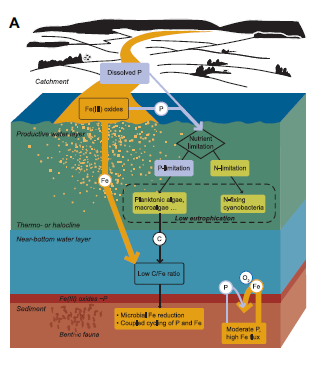
\includegraphics[width=0.8\textwidth]{../Kuvat/eutrophication_A.png}
  \caption{Expected effects of eroded soil on eutrophication on estuary in case of high amount of \ch{Fe} oxide flux \cite{SoilErosion}.}
  \label{fig:eutroA}
\end{figure}

If erosion control measures takes place in the catchment of an estuary, we might see a decrease of \ch{Fe} oxides due to lowered flow of soil, but an increase in dissolved \ch{P}. The increase of \ch{P} is common outcome of reduced tilling. The increased amounts of \ch{P} trigger algal production, which increases the flux of organic \ch{C} to the sediment surface. As the amount of \ch{C} increases the \ch{SO4} reduction becomes more important. The reduction in the \ch{Fe} oxide flux further promotes the importance of \ch{SO4} reduction as the \ch{C}/\ch{Fe} ratio is increased. As \ch{SO4} reduction rate increases, more of the sediment \ch{Fe} is transformed into non-sorptive \ch{Fe} sulfides. Now the "ferrous wheel" is broken and \ch{Fe} bound \ch{P} stored in sediments is released causing the estuary to be highly eutrophic. The benthic fauna of the sediment is largely gone and we might observe large cyonobacterial blooms. This state is difficult to reverse, due to the requirement of a shift in sediment microbial processes and a successful load reduction. This outline is visualized in figure \ref{fig:eutroB}.
\begin{figure}[h!]
   \centering
   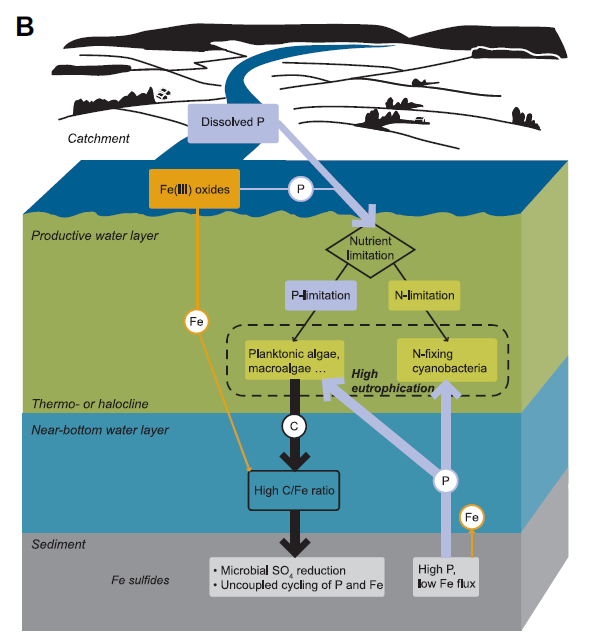
\includegraphics[width=0.8\textwidth]{../Kuvat/eutrophication_B.png}
   \caption{Expected effects of eroded soil on eutrophication on estuary in case of low \ch{Fe} oxide flux \cite{SoilErosion}}
   \label{fig:eutroB}
\end{figure}

The effect of increase in \ch{C} production, caused by \ch{P}, are not straightforward. The settling flux is affected by the hydromorphology and chemistry of the receiving water body. For example in deep systems the \ch{C} is largely mineralized in water phase, and benthic processes are almost non-existent. The depth profile also affects sediment accumulation. Lastly any barriers in \ch{O2} transport to near bottom waters, such as thermocline and halocline, affect the sediment state. 

The availability of \ch{C}, \ch{Fe} and \ch{SO4} are obviously crucial for sediment processes. With low \ch{SO4} levels, the \ch{SO4} reduction plays only minor role. The \ch{P} desorbed in soil particles, in addition to \ch{P} in dissolved form, can be expected to dominate the primary production of algae.

If eroded soil improves the ability of the soil to preserve the \ch{P} by promoting \ch{Fe} reduction and later by coupled \ch{Fe} and \ch{P} cycling, the net effect on eutrophication depends on the balance of following factors:
\begin{enumerate}
\item Mobile soil \ch{P} that can support algal primary production.
\item The lowering of benthic \ch{P} release caused by \ch{Fe} oxides.
\end{enumerate}
The balance is evidentially site-spesific, but it is possible to estimate it by determining the rate of algal-available \ch{P} and the rate of \ch{Fe} that is available for \ch{Fe} reducing microbes in the incoming fluxes.

\section{Vivianite}
Another major component affecting the fate of \ch{P} is hydrated iron phosphate called vivianite ($\ch{Fe3(PO4)2*}8\ch{H2O}$). The long-term storage of phosphorus in marine systems is in sediments. Phosphorus retention in sediment is however limited by the redox dependency. Organic phosphorus under anoxic conditions is remineralised faster relative to organic carbon and iron-oxyhydroxides, bearing phosphorus, undergo dissolution \cite{Vivianite}. Efflux of phosphorus from the seafloor can accelerate eutrophication.     

In Baltic sea the removal of phosphorus is mostly caused by burial of organic matter. However recent observations have shown that vivianite may act as a major sink for phosphorus, as it is buried into the sea bottom \cite{Burial}. Most commonly the precipitation of vivianite observed with high concentrations of pore water iron in the absence of hydrogen in sulfite, such as below the sulphate-methane transition zone \cite{Diagenetic}. Nonetheless recently vivianite has also been observed within the sulphate-methane transition zone in the northern Baltic sea sediments \cite{JILBERT2013155}.

\begin{figure}[h!]
  \centering
  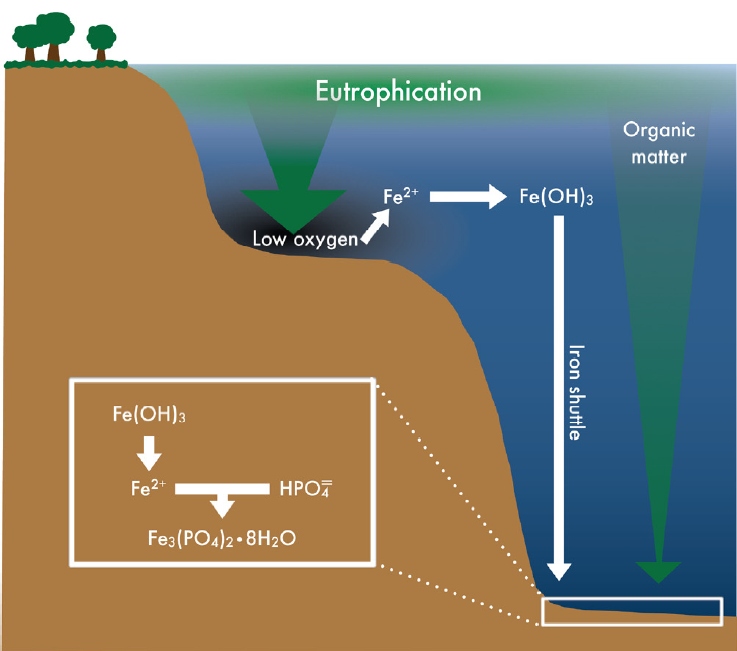
\includegraphics[width=0.4\textwidth]{../Kuvat/vivianiitti.png}
  \caption{Possible processes affecting vivianite formation (plus increases and minus decreases the procution): (A) the reduction of iron by dissimilatory metal reduction bacteria (DMRB), (B1) the anaerobic oxidation of methane (AOM) with iron, (B2) AOM with sulfate, (C) sulfate reduction and (D) sorption and desorption of iron  \cite{ROTHE201651}.}
  \label{fig:vivianiitti}
\end{figure}


The possible cause of the observation was presented by Reed et al in their simulation study \cite{Vivianite}. Their simulation was based on sediment samples taken from one of the deep sea basins of Baltic sea, where oxic and anoxic conditions alter based on major inflow events of dence oxic water from the North Sea.  The possible processes affecting vivianite formation are presented in figure \ref{fig:vivianiitti}.

As a result they noticed that the amount of vivianite found in the sediment was a function of the iron flux settling to the bottom. However the \ch{P} can also be bound in other iron oxyhydroxides, but the vivianite might be one component to look for, when performing the analysis of our samples.    
    

\section{Sediment as a Research Interest}
In this research we are using x-ray absorption spectroscopy to study the sediments in different environments and try to verify if we are able to see any shifts in chemical environment. We try to simulate the path of the soil by first measuring the spectra of different soil types, which have been dried and filtered. Then we are going to mix the soils with Baltic sea waters and vary the level of labile organic \ch{C} and \ch{S}. Lastly we introduce an anaerobic environment. The absorption spectra will be measured in each case and we try to trace whether there is a shift in the chemical state or not. We are expecting the chemical state to remain similar during the two first experiments and in the third one according the outline described in section \ref{Outline}, we are expecting to see how much \ch{Fe} sulfides can be formed by the organic contained by the water and soil itself and then does the addition of organic \ch{C} increase the formation of \ch{Fe} sulfides further.

If our method of sediment research works, it can be applied to measure large set of different water and soil types to further study the effects of soil erosion and agriculture in different water types.

\chapter{X-ray Absorption Spectroscopy}\label{XAS}
X-ray absorption spectroscopy (XAS) focuses on studying how x-rays are absorbed above and below the element specific jumps, or peaks, in the absorption cross-section called absorption edges. XAS allows studying of the local structure around selected element in the sample. XAS does not require long range order, and it can be applied not only to crystals, but also amorphous systems, glasses, quasicrystals, disordered films, membranes, solutions, liquids, metalloproteins, molecular gases etc. These relaxed constraints for the samples make XAS a versatile tool in various fields, such as physics, chemistry, biology, medicine, engineering, environmental science and geology \cite{Fundamentals}.

XAS measurements are relatively straightforward. The main difficulty is obtaining a energy-tunable x-ray source. Since 1970s this has typically meant synchrotron radiation sources, but lately laboratory systems based on analyser crystals have gained some ground due to limited synchrotron beam time and due to increased quality of spherically bent crystals analysers. Many experimental techniques and sample conditions can be applied in XAS measurements, where the most limiting factors are often the energy range, beam size and intensities available from the x-ray source.  

The term XAS, also known as XAFS (X-ray Absorption Fine Structure), is an upper level term for various techniques. XAS is typically divided into the XANES (X-ray Absorption Near Edge Spectroscopy) region, which focuses on the energies at vicinity of the absorption edge, and the EXAFS (Extended X-ray Absorption Fine-structure Spectroscopy), which focuses on the energies well above the absorption edge \cite{Elements}.

\section{X-ray Absorption and Fluorescence} 
X-rays are a form of electromagnetic radiation. Typical X-ray energies range from $\sim\SI{500}{\electronvolt}$ to $\SI{500}{\kilo\electronvolt}$, and wavelengths from $\sim\SI{25}{\angstrom}$ to $\SI{0.25}{\angstrom}$. In the typical X-ray energy range, the photons are absorbed by matter through the photoelectric effect. Electrons are bound in atoms with discrete energies. When an incoming X-ray photon interacts with an atom, the photon can either excite or remove an electron from the atom. In order to an electronic core-level to participate in absorption, the x-ray photon has to have an energy equal to or greater than the binding energy of core level electron.  Released electron is called a photoelectron. 

%Right at   In photo-electric effect an X-ray photon is absorbed by an electron in a tightly bound quantum core level of an atom.

 
  %absorptiokerroin
In a XAS measurement the basic physical quantity to measure is the x-ray absorption coefficient $\mu(E)$, which describes the probability for x-rays to be absorbed as a function of the photon energy. Typically $\mu(E)$ decreases smoothly as energy is increased, approximately as $1/E^3$ \cite{Elements}. However there are sudden jumps in the absorption cross-section at certain energies. These jumps are characteristic to the elements and they occur when the x-ray photon has an equal energy to that of the binding energy of a core-level electron, and they are called absorption edges. 

The absorption coefficient can be obtained from Beer's law:
\begin{equation}\label{eq:beer}
I=I_0e^{-\mu x} \Rightarrow \mu x= ln{\frac{I_0}{I}}, 
\end{equation}
where $I_0$ is the intensity of x-rays incident on a sample, $x$ is the sample thickness and $I$ is the intensity transmitted through the sample.   
For most x-ray energies the absorption coefficient is a smooth function of energy
\begin{equation}
\mu\approx\frac{\rho Z^4}{AE^3},
\end{equation}
where $E$ is the x-ray energy, $\rho$ the sample density, $Z$ the atomic number and $A$ the atomic mass.

%mu ja Z riippuvuus
Absorption coefficient is strongly dependent on both $Z$ and $E$. $Z$ dependence allows the contrast between materials with different densities in typical X-ray image. The $E$ dependence on the other hand allows to obtain a suitable penetration depth into the material, by adjusting the beam energy. These features are useful in medical and other imaging techniques.
%absorptioreuna

As previously stated, there is a sharp rise in absorption when the incident X-ray energy is equal to the binding energy of a core-level electron, which is called the absorption edge. When performing a XAS measurement we are interested in the absorption coefficient $\mu$ as a function of energy at the vicinity of the absorption edge. Every element has well-defined core-level electron binding energies, so in XAS one can select the element of interest by altering the x-ray energy to an appropriate absorption edge. The edge energies vary with atomic number approximately as $Z^2$ \cite{Fundamentals}. 
%viritetty tila
After the atom has absorbed the X-ray photon, the atom is in an excited state. After the absorption event the excited state will typically decay within a few femtoseconds \cite{Elements}. The core hole can decay by two different absorption processes. The first one is X-ray fluorescence, where higher energy electron fills the core hole, and a characteristic X-ray is emitted. The energy of the emitted photon is characteristic to the elements and are tabulated. X-ray fluorescence can be used to identify elements and quantify their concentrations. The second process for the decay is the Auger effect. In the Auger effect an electron falls into the vacancy and the energy is transferred to another electron, which is ejected from the atom into the continuum. X-ray fluorescence occurs with a higher probability in the hard X-ray measurement than the Auger effect, and in case of soft X-rays the Auger effect is more probable. Absorption coefficient $\mu$ can be measured using either of these processes.        

%transmissio ja fluoresenssi
XAS measurement can be done by using transmission or fluorescence geometries. Transmission, which was used in this work is further discussed in section \ref{transmission}. In transmission geometry we can measure energy dependence of absorption coefficient $\mu(E)$ as 
\begin{equation}\label{eq:transmissio}
\mu x=\log(I_0/I) 
\end{equation}
or in fluorescence geometry as 
\begin{equation}\label{eq:fluorescense}
\mu x\propto I_f/I_0
\end{equation}
where $I_f$ is intensity of a fluorescence line.


XAS spectra can be divided in two distinct portions as seen in figure \ref{fig:xassections}. The spectra shows a sharp rise of $\mu(E)$, which is due to $1s$ to $(n+1)p$ transition, and the oscillations of $\mu(E)$, which are the fine-structure. The XANES portion of the spectra is typically within $\SI{30}{\electronvolt}$ of the main absorption edge and the EXAFS region extends typically $500-\SI{1000}{\electronvolt}$ from the XANES portion \cite{Elements}. The EXAFS portion can be interpreted more easily due to some important approximations.  
\begin{figure}[h!]
   \centering
   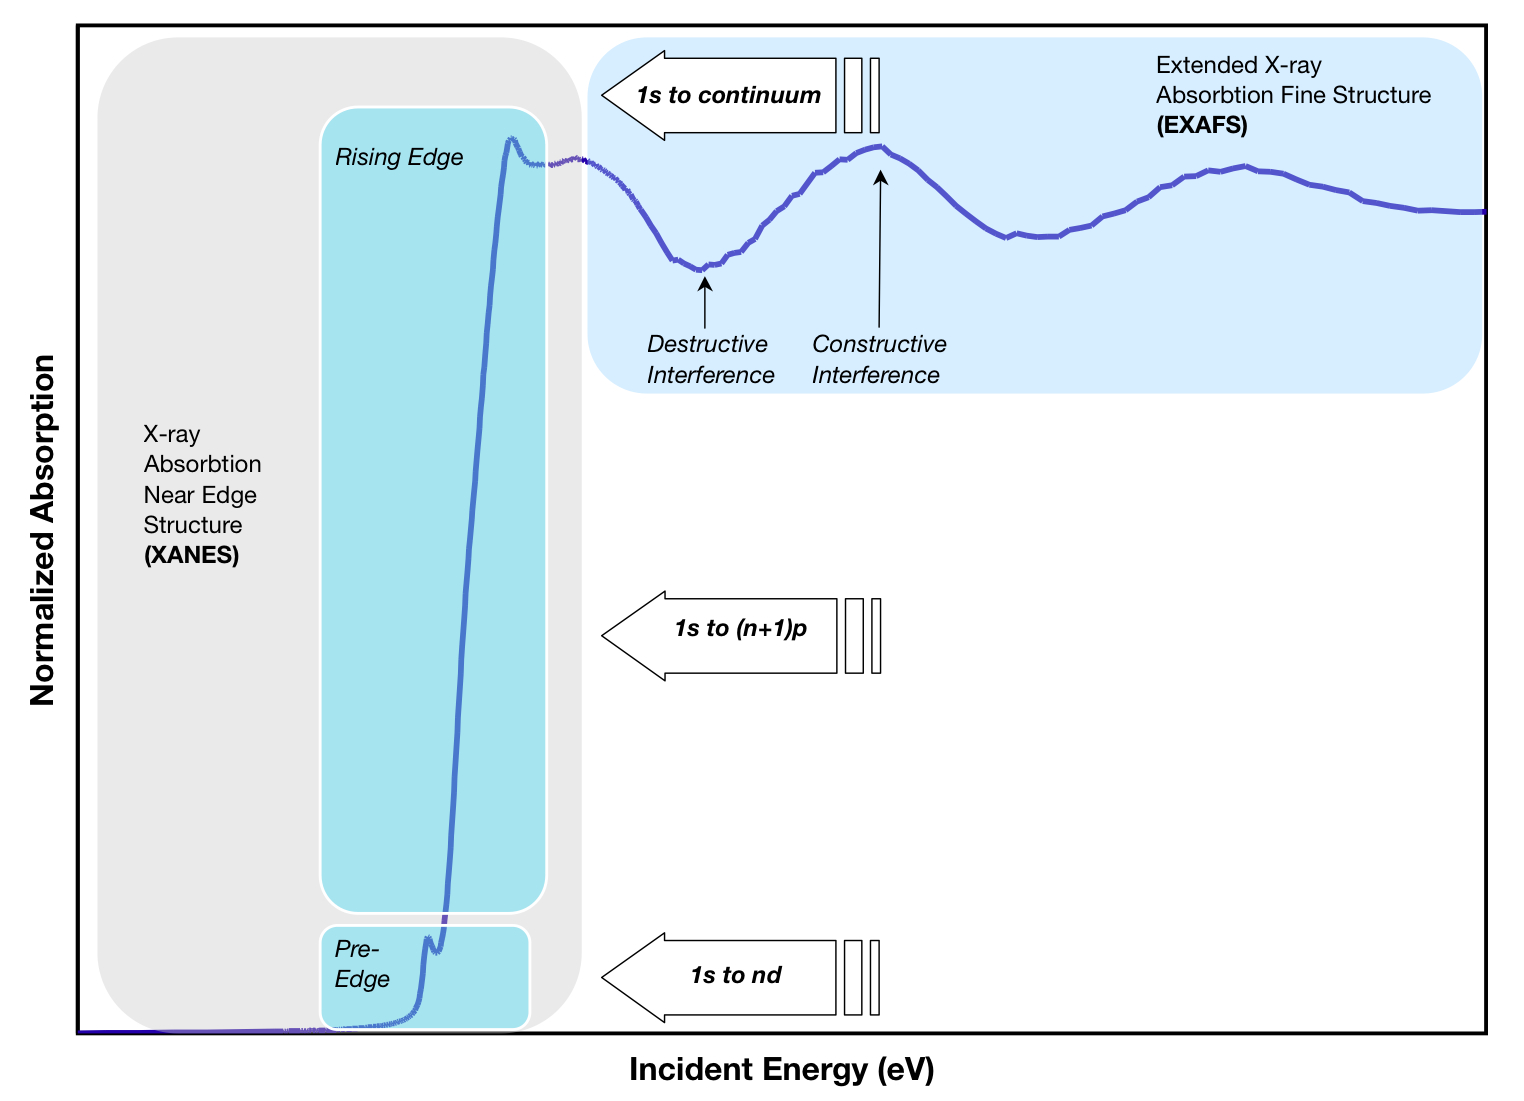
\includegraphics[width=\textwidth]{../Kuvat/XASFig.png}
   \caption{Sections of a typical XAS spectra \cite{wikipedia}.}
   \label{fig:xassections}
\end{figure}

%In EXAFS the main interest are the oscillations well above the absorption edge. The EXAFS fine-structure $\chi(E)$ is defined as 
%\begin{equation}\label{eq:fine-structure}
%\chi(E)=\frac{\mu(E)-\mu_0(E)}{\Delta\mu_0(E_0)}
%\end{equation}
%where $\mu(E)$ is the measured absorption coefficient, $\mu_0(E)$ is a smooth background function describing the bare atom absorption and $\Delta\mu_0$ is the measured jump in the absorption $\mu(E)$ at the threshold energy $E_0$ as seen in figure \ref{fig:typicalxas}.

%\begin{figure}[h!]
%   \label{fig:typicalxas}
%   \centering
%   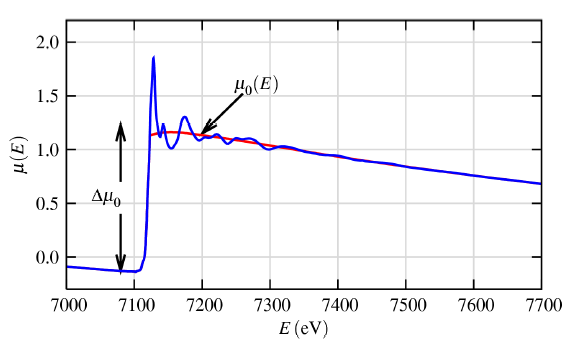
\includegraphics[width=0.7\textwidth]{../Kuvat/xastypical.png}
%   \caption{Smooth background function $\mu_0(E)$ and height of the edge step $\Delta\mu_0(E_0)$}
%\end{figure}

%Instead of photon energy $E$, it is common to use the wave number $k$ of the photo-electron 
%\begin{equation}\label{eq:k}
%k=\sqrt{\frac{2m(E-E_0)}{\hbar^2}}
%\end{equation}
%where $E_0$ is the absorption edge energy and $m$ is the electron mass. The main interest in EXAFS is thus the oscillations as a function of wave-number: $\chi(k)$. $\chi(k)$, often called as "the EXAFS", decays quickly with $k$. The oscillations can be emphasized by multiplying by a power of $k$.

%Different near-neighbour coordination shells correspond to different frequencies observable in the oscillations of $\chi(k)$. This can be modelled by the EXAFS equation: 
%\begin{equation}\label{eq:EXAFS}
%\chi(k)=\sum_j\frac{N_jf_j(k)e^{-2k^2\sigma_j^2}}{kR_j^2}
%\end{equation}
%where $f(k)$ and $\delta(k)$ are scattering properties of the neighbouring atoms, $N$ is the number of the neighbouring atoms, $R$ is the distance of neighbouring atoms and $\sigma^2$ is disorder in the neighbour distance. This equation allows one to determine $N, R$ and $\sigma^2$, and since the scattering amplitude $f(k)$ and phase-shift $\delta(k)$ depend on the $Z$ of the neighbouring atoms, EXAFS is also sensitive to the atomic species of those neighbours.

\section{Theoretical Description of XAS}
Now we'll focus more on the finer details of XAS. In the X-ray absorption a photon is absorbed and a core electron is excited to an unoccupied state, leaving a core hole behind. When the X-ray is absorbed there is a transition to a higher state, or a photoelectron is ejected from the atom. 

\begin{figure}[h!]
  \centering
    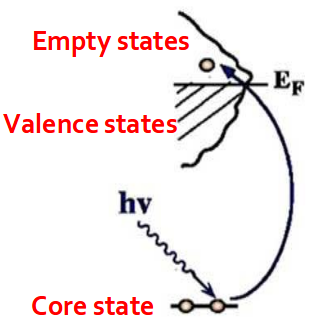
\includegraphics[width=0.4\textwidth]{../Kuvat/absorption.png}
  \caption{In XAS we are measuring the density of states in presence of a core hole. $E_F$ in the figure is the Fermi level \cite{theory}.}
  \label{fig:dos}  
\end{figure}

For optical and X-ray transitions the probability of a transition is obtained by using Fermi's golden rule: 

\begin{equation}
P_{i\rightarrow{f}}\propto|\braket{i|\mathcal{H}|f}|^2\rho_f,
\end{equation}
where $\bra{i}$ is the initial (ground) state, $\ket{f}$ is the final state, $\mathcal{H}$ is the light-matter interaction operator and $\rho_f$ is the density of final states. The wave function of the initial state in spherical harmonics basis is
\begin{equation}
\ket{i}=R^0_{l_0}(r)Y_{l_0,m0}(\theta,\phi),
\end{equation} 
where $R^0_{l_0}(r)$ are the radial functions, $Y_{l_0,m0}(\theta,\phi)$ spherical harmonic functions, $l_0$ angular momentum of the electron. For the final state, if a photoelectron is ejected, we have to take into account that the electron moves in the condensed matter, where the potential of neighbouring atoms is present. The final state is determined by dipole selection rules: $\Delta l=\pm1, \Delta j=\pm1, \Delta s=0$. Primarily for the K- and L$_1$-edges the transitions will be $s\rightarrow p$ and for L$_2$- and L$_3$ edges $p\rightarrow d$. Sometimes transitions are true quadrupolar transitions, which are usually very weak.  

The light-matter interaction operation is obtained from quantum radiation theory:

\begin{equation}
\mathcal{H}=\mathbf{p}\cdot\hat{\varepsilon} e^{i\mathbf{k}\cdot\mathbf{r}},
\end{equation}
where $\mathbf{p}=i\hbar\nabla$ is the momentum operator, $\hat{\varepsilon}$ is polarization vector, $\mathbf{k}$ wave vector of the incident beam and $\mathbf{r}$ the position vector. In case of low momentum, the transfer dipole approximation is used for $\mathcal{H}$:

\begin{equation}
\braket{i|\mathbf{p}\cdot\hat{\varepsilon} e^{i\mathbf{k}\cdot\mathbf{r}}|f}\simeq\hat{\varepsilon}\braket{i|\mathbf{p}|f}.
\end{equation}
The density of final states can be computed by using energy conservation
\begin{equation}
E_f=E_i+\hbar\omega,
\end{equation}
where $E_f$ and $E_i$ are energies of the final and initial state and $\hbar\omega$ is energy of the X-ray photon, and can be noted as

\begin{equation}
\rho_f=\sum_f\delta(E_f-E_i-\hbar\omega),
\end{equation} 
where the contribution of each possible final state is taken into account. 
 
The absorption coefficient depends on the absorption probability, and it can also be described with Fermi's golden rule:

\begin{equation}\label{eg:golden}
\mu(\omega)\propto\sum_f|\braket{i|\mathbf{p}\cdot\hat{\varepsilon} e^{i\mathbf{k}\cdot\mathbf{r}}|f}|^2\delta(E_f-E_i-\hbar\omega),
\end{equation}
where we sum over all possible final states. This form is called one-electron golden-rule approximation. Solving the Fermi's golden rule in a way or another is the key to theoretically interpret both XANES and EXAFS. There is no single way to do this if we want to cover the whole absorption spectra. We have to rely on different paths to explain different sections of the spectra, and also introduce more complicated models to take into account for example many-body effects \cite{theory}.

%The X-ray absorption is a transition between two quantum states, $\bra{i}$ and $\ket{f}$, and can be described with Fermi's golden rule \cite{Fundamentals}:
%\begin{equation}
%\mu(E)\propto|\braket{i|H|f}|^2
%\end{equation}
%In the initial state $\bra{i}$ we have an X-ray, core-electron and no photo-electron, and in the final state $\ket{f}$ no X-ray, a core hole and a photo-electron. The interaction term $H$ can be obtained from quantum radiation theory \cite{Fundamentals}, an is the $\mathbf{p}\cdot\mathbf{A}$ term. $\mathbf{A}$ is quantized vector potential and $\mathbf{p}$ the angular momentum. When calculated open, the term reduces to a term which is proportional to $e^{ikr}$. 

%We can apply the Fermi's golden rule to both EXAFS and XANES region. In XANES we have to either apply molecular orbital theory or multiple scattering theory into our picture to estimate $\mu{E}$. This is very difficult to do analytically and often done computationally. In the EXAFS region we notice that there is relationship between $\mu(E)$ and the fine-structure $\chi(E)$:

%\begin{equation}
%\mu(E)=\mu_0(E)[1-\chi(E)],
%\end{equation}
%where $\mu(E)$ is the "bare-atom absorption".


%X-ray absorption is a transition between two quantum states. In the initial state an x-ray, a core-electron, and no photo-electron are expected, and in the final state no x-ray, a core hole and a photo-electron. With the initial and final state we can describe the $\mu(E)$ with Fermi's Golden Rule

%\begin{equation} \label{eq:Fermi}
%\mu(E) \propto |\braket{i | H | f}|^2
%\end{equation}
%where $\bra{i}$ is the initial state, and the $\ket{f}$ the final state, and $H$ is the Hamiltonian representing the interaction. The core-electron is tightly bound in the absorbing atom, so the initial state is not altered in the presence of a neighbouring atom. However the photo-electron will be able to see the neighbouring atom and thus the final state will be affected. By expanding the $\ket{f}$ into two pieces, $\ket{f_0}$ that represents the bare atom portion and the $\ket{\Delta f}$ represents the neighbouring atom, we get  


%\begin{equation}
%\ket{f}=\ket{f_0}+\ket{\Delta f} 
%\end{equation}
%which can be applied to equation \ref{eq:Fermi}
%\begin{equation}
%\mu(E)\propto |\braket{i | H | f}^2[1+\braket{i|H|\Delta f}\frac{\braket{f_0|H|i}^*}{|\braket{i|H|f_0}|}+C.C]
%\end{equation}
%where $C.C.$ stands for complex conjugate. This resembles the closely previously discussed relation between $\mu(E)$ and $\chi(E)$  
%\begin{equation}
%\mu(E)=\mu_0(E)[1+\chi(E)].
%\end{equation}

%Combining the previous equation allows us to assign $\mu_0=|\braket{i|H|f_0}|^2$ as the bare atom absorption, which depends only on the absorbing atom. We also note that the fine-structure $\chi$ can be written as
%\begin{equation}
%\chi(E)\propto\braket{i|H|\Delta f}.
%\end{equation}



\section{XANES}
In XANES we focus on the features right around the edge and up to a few dozens electronvolts above the edge. The XANES region is much easier to measure than the EXAFS region. This is mainly due to the fact that the intensity oscillations are larger and the energy range is smaller. XANES can be done with lower concentrations and the restrictions in sample constrains are not as tight as in EXAFS.  

Typical XANES spectra can be roughly divided into a few specific regions. The pre-edge, shown in figure \ref{fig:XANESfetures} as the red region, may exhibit small features corresponding to (bound) $1s\rightarrow 3d$ transitions (states). The edge or the rising edge, the purple section in figure \ref{fig:XANESfetures}, is the main rising part of XANES spectra. Near-edge is the green part in figure \ref{fig:XANESfetures}. 

\begin{figure}[h!]
  \centering
  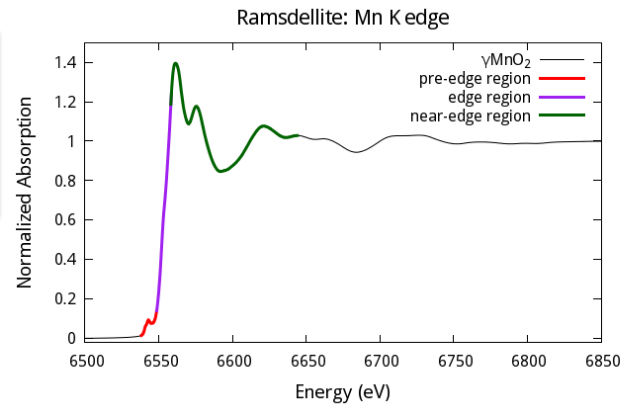
\includegraphics[width=\textwidth]{../Kuvat/XANESparts.png}
  \caption{Different features in the XANES region \cite{Ravel}.}
  \label{fig:XANESfetures}
\end{figure}
In the pre-edge and edge region we deal with bound state transitions and in the near edge region the X-ray photon has enough energy to eject the electron with low kinetic energy, and it strongly scatters from the neighbouring atoms.

Qualitatively XANES can used as a fingerprint of the electronic structure. These fingerprints can be compared to known model complexes. Fingerprints and known reference samples can be compared with principal component analysis, or with least square linear combination fitting, to determine the chemical composition of the sample. Other important qualitative pieces of information we can obtain are oxidation number, coordination, core-hole effects, charge transfer, projected density of states and dipole matrix elements. These will be covered more in detail in the following sections.

In order to get more quantitative results we can try to solve the Fermi's golden rule by using various techniques. In case of bound state transitions a common way is to use molecular orbital theory, or density functional theory to represent the final state, and solve the integral. This works well for ground-state properties and for the pre-edge region. If the photoelectron has enough energy to excite a low energy photo-electron, we can use multiple scattering, also known as Green's function formalism. We will represent these two method briefly in the following sections.

Other methods to solve Fermi's golden rule have been developed. Method's like Bethe-Salpeter equation \cite{theory}, which is derived using quantum field theory, and Real-time method \cite{theory}, which simulate the wave functions as a function of time instead of energy space, have been used, but will not be discussed in this work.

%one can use molecular orbital-based approach. This method works when analysing the pre-edge and the bound state transitions. By using ligand field theory one can understand the energy and and intensity distribution of the pre-edge\cite{Hahn}. In order to get a grasp of rising edge and the near-edge, one can use multiple-scattering approach to simulate the structure. Multiple-scattering approach can be difficult to relate back to the molecular orbital-based picture \cite{Slac}.

\subsection{Wave Function Methods for Fermi's Golden Rule}
Another form of Fermi's golden rule is to represent it the integral form

\begin{equation}
\mu\propto|\int \psi_f^*\hat{\varepsilon}\cdot\mathbf{r}e^{i\mathbf{k}\cdot\mathbf{r}}\psi_i d^3r|^2\rho_f
\end{equation}
which we can approximate in terms of dipole and quadrupole terms:
\begin{equation}
\approx|\int \psi_f^*(\hat{\varepsilon}\cdot\mathbf{r} +i(\hat{\varepsilon}\cdot\mathbf{r})(\mathbf{k}\cdot\mathbf{r}))\psi_i d^3r|^2\rho_f.
\end{equation}
This matrix element projects out the part of the final state that is of the right symmetry (dipole selection rules). With a careful analysis we can try accurately present both the initial and final state to solve this integral directly. This can be done for example by using single Slater determinant, or with time-dependent density functional theory \cite{theory}. This method suitable for analysis, when the photoelectron is not present. In order to succeed, core basis set and valance basis sets have to be selected successfully.  

\subsection{Bound State transitions}
In the figure \ref{fig:XANESfetures} we see a weak pre-edge peak. The pre-edge peak is caused by bound state transitions. The pre-edge is not always a simple bump in a spectra, it might have a more complicated shape, as seen in figure \ref{fig:pre-edge}. This intensity pattern is a result of multiplet structure. The spin state, oxidation state, ligand-field splitting and multiplet-effects can all affect the pattern \cite{Slac}. By taking intensity-weighted average energy of the pre-edge, one can notice, that it is modulated by ligand-field strength \cite{Slac}. To perform this kind of analysis on the pre-edge, one needs a high quality measurement with very little noise, since the features of the pre-edge can be rather small.
\begin{figure}[h!]
  \centering
    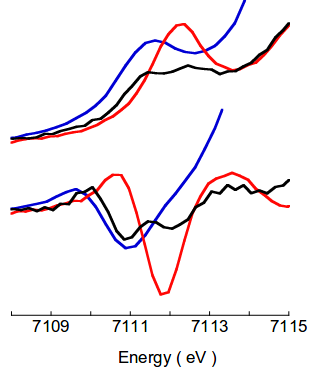
\includegraphics[width=0.6\textwidth]{../Kuvat/pre-edge.png}
  \caption{The pre-edge features of certain XANES-spectra above, and intensity-weighted average energy below \cite{Slac}.}
  \label{fig:pre-edge}
\end{figure}

In case of K edge of a first row transition metal, the peak is caused by $1s\rightarrow 3d$ transition \cite{Hahn}. The $1s\rightarrow 3d$ transition is not allowed transition according to dipole selection rule, but it is still observed due to $3d+4p$ mixing and to direct quadrupolar coupling. We can use intensity of the $1s\rightarrow 3d$ transition into our advantage to determine the geometrical structure. As the $3d+4p$ mixing improves the $1s\rightarrow 3d$ transitions increase as well, which can be used as a tool to determine bond symmetry, for example tetrahedral or octahedral \cite{Hahn}. In some cases the bond symmetry can also be an indicator for valence \cite{Slac}. $1s\rightarrow 3d$ transitions have also been used in electronic band structure calculations since band structure calculations also involve multiple-scattering paths of electrons in a solid similar to XANES \cite{Xas}.  


Sometimes it is also possible to probe higher-lying exited states with XANES. For the first row transition series metals the $1s\rightarrow 4p$ transition is dipole allowed, and is over two orders of magnitude more intense than the pre-edge. Typically the transition is obscured by the rising edge, and often not observed. There are exceptions however, like the ones of \ch{Cu}(I) and \ch{Zn}(II) complexes \cite{SARANGI2013459}. In their case the $1s\rightarrow 4p$ transition arise an intense feature on the rising edge, as seen in figure \ref{fig:1s4p}.

\begin{figure}[h!]
   \centering
      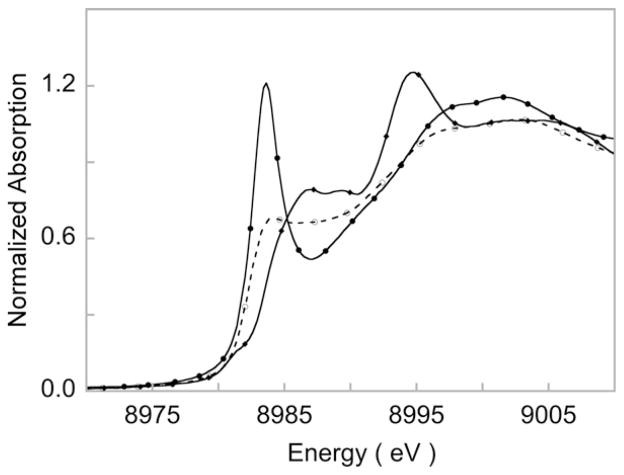
\includegraphics[width=0.8\textwidth]{../Kuvat/1s_4p.png}
   \caption{\ch{Cu} K-edge spectra of \ch{Cu}(I) complexes. Two-coordinate system shows a simple rising edge, but in case of three-coordinate and 4-coordinate system there is a shoulder which arise from the $1s\rightarrow 4p$ transition \cite{SARANGI2013459}.}
   \label{fig:1s4p}
\end{figure}  
  
A complimentary approach to the metal XANES is to use ligand XANES to study the electronic structure \cite{Hahn}. For example in case of sulphur or chlorine ligands the amount of metal-ligand orbital mixing (i.e. covalency) can be quantitated by this approach. In case of metal chlorides the bonding orbital is \ch{Cl} 3p, and the lowest energy transition is $1s\rightarrow\mathrm{HOMO}$ (highest occupied molecular orbital), where the HOMO can have a character of both ligand \ch{Cl} $3p$ and metal $3d$. The $1s\rightarrow\mathrm{HOMO}$ is thus direct measurement of the percent of $3p$ character in HOMO.

%In a case of ligand XANES we are interested in $1s\rightarrow 3p$ transition for \ch{S} and \ch{Cl}, which is allowed transition and much easier to detect, than the $1s\rightarrow 3d$ transition in case of metal XANES  
%In case of the second row transition metals the $1s\rightarrow 4d$ transition is tricky to measure. Edge energies are higher, which decreases the core-hole lifetime, and at higher energies monochromator resolutions tend to be poor. As a result the edges are broader and the $1s\rightarrow 4d$ transition is undetectable.

\subsection{Multiple Scattering Events}
When the X-ray photon has barely enough energy to excite a photo-electron, the photo-electron has low energy and longer mean free path. Now the photo-electron can be scattered by more atoms than a single one. In fact photo-electron can be scattered by two or more atoms prior to returning to the absorbing atom, as seen in figure \ref{fig:ms}. 

In order to calculate the XAS spectrum, we have to introduce multiple scattering formalism \cite{theory}. We'll start by rearranging the equation \ref{eg:golden}:

\begin{equation}\label{eq:mod_golden}
\mu(\omega)\propto\sum_f|\braket{i|\mathcal{H}|f}|^2\delta(E_f-E_i-\hbar\omega)=\braket{i|\mathcal{H}\sum_f|f}\braket{f|\delta(E_f-E_i-\hbar\omega)\mathcal{H}^{\dagger}|i}
\end{equation} 
Now we can notice the similarity of Green's function:
\begin{equation}
G(\omega)=\sum_f\frac{\ket{f}\bra{f}}{E-E_F}.
\end{equation}
With a small rearrangement of the Green's function we get
\begin{equation}
-\frac{1}{\pi}\operatorname{Im}G(\omega)=\sum_f\ket{f}\bra{f}\delta(E_f-E_i-\hbar\omega).
\end{equation}
This form we can now apply to equation \ref{eq:mod_golden} and we get
\begin{equation}
\mu(\omega)\propto-\frac{1}{\pi}\operatorname{Im}\braket{i|\hat{\varepsilon}\cdot\mathbf{r}G(\omega)\hat{\varepsilon}\cdot\mathbf{r}^{*}|i}\Theta_\Gamma(E-E_F),
\end{equation}
where $\Theta_\Gamma(E-E_F)$ is a broadened step function at the Fermi energy $E_F$. The difficulty in this formalism is computing the Green's function. The Green's function here describes all possible ways for photo-electron to interact with the surrounding atoms. In the XANES region the way forward is brute force matrix algebra, which causes limitations to the energy and cluster sizes. 

For condensed matter a simple approximation can be used: Spherical atomic like potentials centred on each atomic site, and outside of those sites potential is set to zero, provide the scattering potentials. With this so called "muffin-tin" potential we can use the following form for Green's function:

\begin{equation}
G=(1-G^0t)^{-1}=G^0+G^0tG^0+G^0tG^0tG^0+G^0tG^0tG^0tG^0+...,
\end{equation}  
where $G^0$ is a function that describes how an electron propagates between two points in space, and $t$ is a function that describes how a photo-electron scatters from neighbouring atoms. This is typically solved computationally, and common softwares like FEFF and FDMNES utilise this method. They often provide good approximations of the spectra.

%The XANES region is sensitive to multiple scattering events, since the the photo-electron has a low kinetic energy and the mean free path is increased. Multiple scattering events complicate simulation of XANES, since there are more interactions and large number of multiple scattering pathways. Even though the multiple scattering events complicates simulations, they also provide a possibility to extract information about the three-dimensional structure from XANES spectra \cite{Fundamentals}. 

%In XAS we measure transition of an electron from a core state $\ket{i}$ into an unoccupied state $\ket{f}$:

%\begin{equation}
%\mu(E)\propto\sum^{E_f>E_F}_f |\braket{i|\hat{\epsilon}\cdot\mathbf{r}|f}|^2\delta(E_f),
%\end{equation}   
%This equation is called Fermi's golden rule \cite{Fundamentals}, and there are two ways to work out the equation. The first one is to accurately represent $\ket{i}$ and $\ket{f}$ and then solve the integral. The initial state is straight forward to represent by using quantum mechanics, but the final state not so much and requires lot's of computations. This approach is taken in by molecular orbital theory \cite{Ms}. The other way is to use multiple scattering theory \cite{Ms}, also known as Green's function formalism:

%\begin{equation}
%\mu(E)\propto-\frac{1}{\pi}\operatorname{Im}\braket{i|\hat{\epsilon}^*\cdot \mathbf{r}G(r,r';E)\hat{\epsilon}\cdot\mathbf{r}'|i}\Theta(E-E_F),
%\end{equation}   
%where $G$ is the Green's function, and $\Theta$ step function, which ensures that only excitations to free states above the Fermi energy $E_F$ are considered. In this approach the difficult part is computing the Green's function. In XANES the function used describes all possible ways for photo-electron to interact with the surrounding atoms. In this case the only way forward is brute force matrix algebra, which causes obvious limitations to energy and cluster sizes.   

%Multiple scattering theory is used in common softwares like FEFF and MXAN to simulate the specta. Recently the simulations have become more and more accurate \cite{Hahn}, but most of the simulations still remain qualitative.

\begin{figure}[h!]
  \centering
  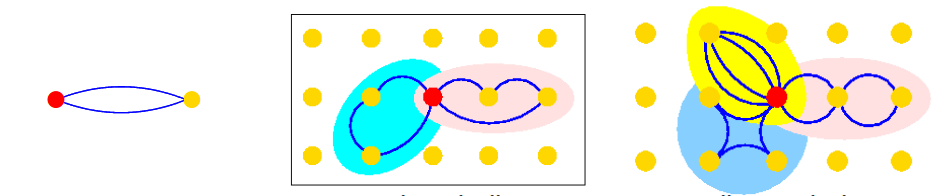
\includegraphics[width=\textwidth]{../Kuvat/multiplescattering.png}
  \caption{There are various scattering paths for a photo-electron to scatter, which complicates calculations of XANES \cite{Ms}. Red atom is the absorbing one and the photoelectron can scatter from the neighbouring yellow sites.}
  \label{fig:ms}
\end{figure}

The changes in the three-dimensional structure can be seen empirically in the XANES spectra. Even small variations in structure can be seen in spectra, and for example two sites with identical EXAFS spectra can have distinct XANES spectra. Geometrical differences between sites alter the multiple scattering pathways, and this at least partly explains the site sensitivity of XANES \cite{Hahn}. The interpretation of XANES spectra has been progressing steadily, and the agreement between computed and measured spectra has increased. The development of theoretical and computational model for detailed interpretation of XANES spectra remains one of the main challenges in the field.

\subsection{Oxidation Number}


The exact energy of the absorption edge can be defined in various ways. Typically it is defined as half height of the edge or as maximum of the first derivative with respect to energy. Often the definition is not as straightforward, since the edge spectra might have unresolved transitions superimposing on the rising edge. These make the definition of a unique edge energy rather troublesome. However, the edge energies are useful tool for determination of oxidation state of the absorption site. The energy of an edge increases as oxidation state of the absorber increases. Atoms with a higher oxidation state should have a higher charge, and to eject a core electron, a higher energy x-rays are needed \cite{Hahn}. 

Alternatively we can treat the edge features as continuum resonances \cite{Hahn}. A continuum resonance involves excitation of a core electron into a high-energy state, above the continuum, with a finite lifetime. Let's use the potential well between absorbing and scattering atoms as an example. As the distance between the atoms gets shorter, the energy of the continuum state increases as $1/R^2$. Higher-oxidation-state metals have shorter bond lengths. This model also predicts the increase in edge energetic with increasing oxidation state. The remark of higher oxidation number increasing the edge energy is widely used in coordination chemistry.

\begin{figure}[h!]
  \centering
  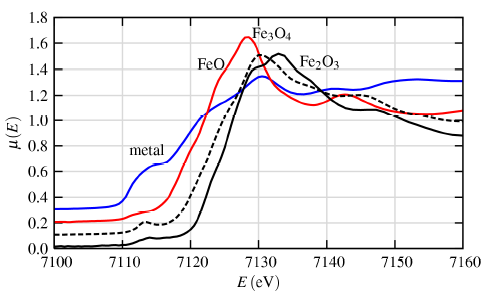
\includegraphics[width=\textwidth]{../Kuvat/FeOxidation.png}
  \caption{\ch{Fe} $K$-edge XANES spectra of metallic \ch{Fe} and some \ch{Fe} oxides. The graph clearly shows relation between oxidation state and edge energy \cite{Fundamentals}.}
  \label{fig:FeOxidation}
\end{figure} 

The figure \ref{fig:FeOxidation} is a great example of the valence dependence of the metallic \ch{Fe} and other \ch{Fe} oxides. With good quality reference samples it is easy to determine the ratios of different oxides in the sample.

\subsection{White Line}
In some XANES spectra, the rising absorption edge might lead to a sharp intensity peak (seen in figure \ref{fig:whiteline}), which arises from the $1s\rightarrow(n+1)p$ transition. This peak is called the white line, reason being that in the past X-ray absorption spectra was recorded on photographic plates. The strong absorption of certain wavelengths lead to an unexposed band on the photographic plates, and when the plate is developed in negatives, band appears as white vertical stripe \cite{Fundamentals}. 

\begin{figure}[h!]
  \centering
    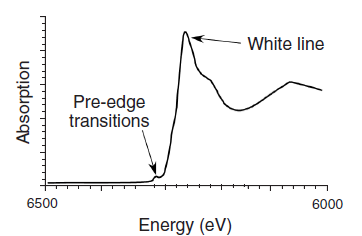
\includegraphics[width=0.5\textwidth]{../Kuvat/whiteline.png}
  \caption{The white line in XANES spectra \cite{Fundamentals}.}
  \label{fig:whiteline}  
\end{figure}

The intensity of the white line depends on the matrix element of Fermi's golden rule, and the occupancy of the bound final states. The matrix element depends on the overlap of the wave functions. And since transitions are forbidden into filled orbitals, due to Pauli's exclusion principle, filling of orbitals suppresses white line.          

\subsection{Multi-Electron Transitions}
At higher photon energies it is possible that X-ray has enough energy to excite an extra electron into the valence band, resulting in double excitation. It is also possible, that continuum states contribute to multi-electron excitations. This multi-electron excitation is also referred to as a shake-up transition \cite{Hahn}.

There is also another class multi-electron excitations. In this case the excitation of a core electron has the effect of converting an atom with atomic number $Z$ into an atom with atomic number $Z+1$. For example in case of $\ch{Cu}^{II}$ in the $\underline{1s}4p^I$ state, the valence electrons experience the effective nuclear charge transfer of $\ch{Zn}^{II}$. This makes the $\underline{1s}3d^94p^1$ transition and multi-electron $\underline{1s}3d^{10}4p^1\underline{L}$ transition possible, where ligand electron has been transferred to a lower energy \ch{Cu} 3d orbital. In this case the multi-electron transition is called the shake-down transition. The shake down transitions are often observed in photoelectron spectroscopy and in resonant inelastic X-ray scattering, and can have a role in XANES as well (in case of $\ch{Cu}^II$ there is good theoretical and experimental evidence of shake-down transitions \cite{Hahn}).   

\section{EXAFS}
In the EXAFS region the X-ray photon has enough energy to excite a photoelectron with a de Broglie wavelength $\lambda=h/p$ corresponding to a transition to continuum (figure \ref{fig:free atom}). 
\begin{figure}[h!]
  \centering
  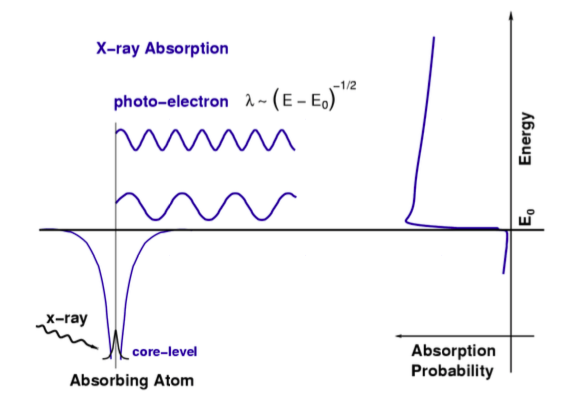
\includegraphics[width=0.8\textwidth]{../Kuvat/absorption1.png}
  \caption{When the incident photon has the energy of a tightly bound electron level, $E_0$, the absorption probability has a clear edge. The tightly bound core level is destroyed in the process and a photo-electron is created. The photo-electron travels as a wave with wave number proportional to $\sqrt{(E-E_0)}$ \cite{Fundamentals}.}
  \label{fig:free atom}
\end{figure}

If we include one neighbouring atom into our picture, the photo-electron can now scatter from the electrons of the neighbouring atom. There is a phase shift associated with the scattering event, causing outgoing and scattered waves to interfere. The constructive and destructive interference at the absorbing atom, caused by the back-scattered photo-electron, will vary with energy. This will cause oscillations in the $\mu(E)$, which is the origin of the fine-structure \cite{Ravel}. The interaction with the neighbouring atom is displayed in figure \ref{fig:neighbour atom}.
\begin{figure}[h!]
  \centering
  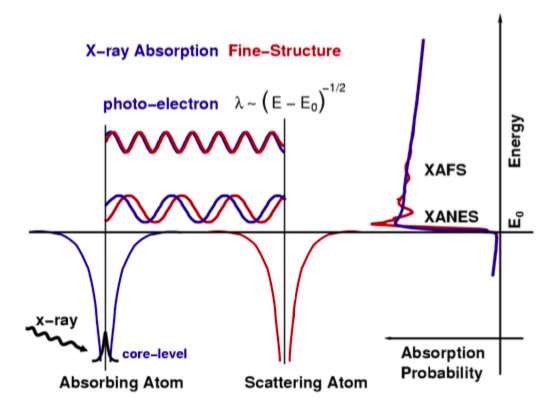
\includegraphics[width=0.8\textwidth]{../Kuvat/absorption2.png}
  \caption{When a neighbouring atom is added to the picture, photo-electron can back-scatter and interfere with the outgoing electron wave, which causes a fine-structure to appear \cite{Fundamentals}.}
  \label{fig:neighbour atom}
\end{figure}
In the EXAFS region we can thus express $\mu(E)$ in terms of fine-structure $\chi(E)$:

\begin{equation}
\mu(E)=\mu_0(E)[1-\chi(E)],
\end{equation}
where $\mu(E)$ is the "bare-atom absorption".

In EXAFS the main interest are the oscillations well above the absorption edge. The EXAFS fine-structure $\chi(E)$ is defined as 
\begin{equation}\label{eq:fine-structure}
\chi(E)=\frac{\mu(E)-\mu_0(E)}{\Delta\mu_0(E_0)}
\end{equation}
where $\mu(E)$ is the measured absorption coefficient, $\mu_0(E)$ is a smooth background function describing the bare atom absorption and $\Delta\mu_0$ is the measured jump in the absorption $\mu(E)$ at the threshold energy $E_0$ as seen in figure \ref{fig:typicalxas}.

\begin{figure}[h!]
   \label{fig:typicalxas}
   \centering
   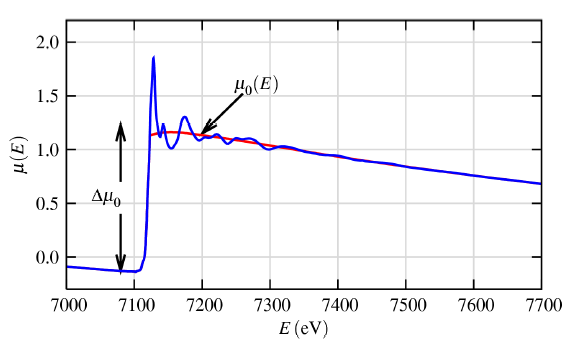
\includegraphics[width=0.7\textwidth]{../Kuvat/xastypical.png}
   \caption{Smooth background function $\mu_0(E)$ and height of the edge step $\Delta\mu_0(E_0)$ \cite{Fundamentals}.}
\end{figure}
   

Instead of photon energy $E$, it is common to use the wave number $k$ of the photo-electron 
\begin{equation}\label{eq:k}
k=\sqrt{\frac{2m(E-E_0)}{\hbar^2}}
\end{equation}
where $E_0$ is the absorption edge energy and $m$ is the electron mass. The main interest in EXAFS is thus the oscillations as a function of wave-number: $\chi(k)$. $\chi(k)$, often called as "the EXAFS", decays quickly with $k$. The oscillations can be emphasized by multiplying the EXAFS spectrum by a power of $k$.

Different near-neighbour coordination shells correspond to different frequencies observable in the oscillations of $\chi(k)$. This can be modelled by the EXAFS equation \cite{Fundamentals} 
\begin{equation}\label{eq:EXAFS}
\chi(k)=\sum_j\frac{N_jf_j(k)e^{-2k^2\sigma_j^2}}{kR_j^2}
\end{equation}
where $f(k)$ is the scattering amplitude and $\delta(k)$ the phase shift, $N$ is the number of the neighbouring atoms, $R$ is the distance of neighbouring atoms and $\sigma^2$ is disorder in the neighbour distance. This equation allows one to determine $N, R$ and $\sigma^2$, and since the scattering amplitude and phase-shift depend on the $Z$ of the neighbouring atoms, EXAFS is also sensitive to the atomic species of those neighbours.

The EXAFS equation breaks down in the XANES region, at low $k$ values, mainly due to the $1/k$ term and the increase in the mean-free-path at very low $k$ (This however doesn't mean that we couldn't draw any conclusion from the XANES spectra, since there is much chemical information in the XANES region. Most notably the sensitivity to oxidation number).

\section{Measuring the Transmission}\label{transmission}
In order to measure the absorption coefficient accurately, few components are essential. XAS is performed with an x-ray source that provides large range of wavelengths, from which a monochromator selects a particular energy. Monochromators are typically made of high-quality single crystals, such as silicon or germanium, and the characteristics of a monochromator can greatly influence the measurement quality. Reproducibility and stability of the monochromator along with its energy resolution are particularly important in XAS measurement. Sufficient energy resolution for XAS is $\sim 1 \si{\electronvolt}$ at $10 \si{\kilo\electronvolt}$. Another important component is the detector, which should have a large dynamic range and it preferably should be energy dispersive in order to discriminate background from monochromator harmonics. 

To further increase the accuracy of the measurement the beam should be well aligned, and the sample should be homogeneous and free from pinholes. In an adequate measurement the noise levels should be $10^{-3}$.

Samples with large concentrations of the element of interest should be measured in transmission. The thickness of the sample obviously affects the transmission, so the sample should be thin enough for decent signal. From equation \ref{eq:beer} we get $x=\ln{(I/I_0)}$ for the thickness. The thickness is typically chosen so that we get $\mu x\approx2.5$ above the edge and/or $\Delta\mu(E)x\approx1$ edge step. In our case we use dilute solutions, so the sample thickness can be in the millimetre range.

When all these factors are taken into consideration, the transmission measurement is rather straightforward and one should easily obtain good quality data. 

\chapter{Spectrometer}\label{setup}
\section{Setup}
We use the X-ray absorption spectrometer, found in the X-ray Laboratory of University of Helsinki, to perform our measurements. The equipment was built by the X-ray Laboratory staff. The instrument is based around three basic components: x-ray tube, a monochromator and a scintillator counter (detector). The monochromator crystal is placed on a motorized rail, and it can also be rotated around its vertical axis essentially to change the angle of the monochromated beam. The detector is also placed on two motorized rails to allow the movement in two dimensions. The x-ray tube is fixed in position. These components follow the so called Rowland circle geometry. Rowland circle is a Bragg reflection geometry, which allows simultaneous focusing and energy analysis of the fluorescence source. The setup is shown in figure \ref{fig:setup}.  

\begin{figure}[h!]
  \centering
  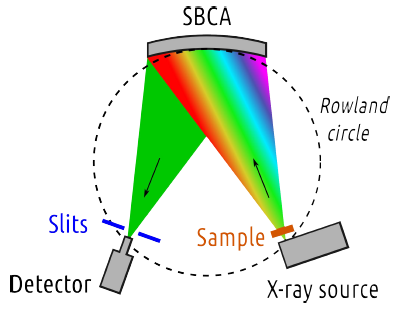
\includegraphics[width=0.8\textwidth]{../Kuvat/helxasSetup.png}
  \caption{Illustration of the measurement setup. SBCA stands for spherically bent crystal analyser \cite{Spektrometri}.}
  \label{fig:setup}
\end{figure}
\subsection{X-ray Source}
The spectrometer is designed to measure X-ray absorption edges in the energy range $\approx 4-\SI{25}{\kilo\electronvolt}$. The x-ray source is a conventional $\SI{1.5}{\kilo\watt}$ fine focus diffraction glass tube with a \ch{Ag} target. \ch{Ag} has characteristic lines above $\SI{20}{\kilo\electronvolt}$ \cite{Spektrometri}, which extends the Bremsstrahlung region up to \ch{Mo} K edge in the periodic table. The source is suitable for e.g. $3d$ transition metal K edge and $5d$ L edge spectroscopy. 



      
\subsection{Monochromators}
The X-rays spectra produced by the X-ray tube is polychromatic and monochromatized by a spherically bent crystal analyser (SBCA). The crystal is used for point-to-point scanning, where a small energy bandwidth ($<\SI{5}{\electronvolt}$) satisfies Bragg's diffraction condition over the entire crystal area and is focused on the detector \cite{AnalyzerCrystal}. The Bragg's diffraction condition is
\begin{equation} \label{eq:bragg}
2d_{hkl}\sin\theta_b=n\lambda,
\end{equation}
where $d_{hkl}$ is the distance between atoms in a lattice, $n$ is an integer, $\theta_b$ is the angle between incident beam and diffracted beam and $\lambda$ is the wavelength of the diffracted beam. The distance $d_{hkl}$ is depends on the Miller indices, and by selecting the right crystal orientation we can also select the wanted energy bandwidth in a point-to-point measurement. The wavelength is related to energy by 
\begin{equation}
\lambda=\frac{hc}{E},
\end{equation} 
where $h$ is Planck's constant and $c$ speed of light in a vacuum. 

For our measurement we use an analyzer crystal with Miller indices $hkl=[3,5,1]$, which allows us to scan the around the K-absorption edge of \ch{Fe} at $E=\SI{7.1}{\kilo\electronvolt}$, by varying the angle $\theta$.

The analyser crystal is spherically bent to focus the beam to the detector. Our setup uses crystals with $\SI{0.5}{\metre}$ bending radius. Spherical bending however causes strain fields in the monochromator, which can alter energy resolution. Strain field effect is addressed by cutting the surface in $\SI{15}{\milli\metre}$ wide strips. The typical energy resolution of our analysers is $\gtrsim \SI{1}{\electronvolt}$. Our strip-bent spherically bent crystal analysers (SBCA) are provided by ESRF Crystal Analyser Laboratory.        

\subsection{Detectors}
The spectrometer can be operated in transmission, fluorescence and imaging modes. The data can also be acquired with multiple detectors. In our case we are using the transmission mode, in which we use a scintillator detector with a single channel analyser. The setup uses doped \ch{NaI} crystal, which converts the x-ray photons to low energy photons, which are converted to a cascade of electrons. These pulses are collected and transformed into voltage pulses. Pulses are proportional to photon energy, and the energy resolution is $\sim30\%$.

The detector has a finite response time to incident photons, known as dead time $\tau$. During that time the detector cannot count other photons. For sufficiently small dead time we can use the following correction

\begin{equation} \label{eq:deadtime}
N_{correct}\approx\frac{N}{1-\frac{\tau}{T}N},
\end{equation}
where $N$ is the number of counted pulses and $T$ is the time in which they were acquired. Dead time of our detector is $\tau=\SI{2.8}{ \milli\second}$.

\subsection{Motors and movements}
Movements of the motors follow the Rowland circle geometry. The setup has three motorized linear translational stages, one motorized goniometer and one passive rotational stage with telescopic with steering bar. 3D model of the components is displayed in figure \ref{fig:cad}. 

\begin{figure}[h!]
  \centering
  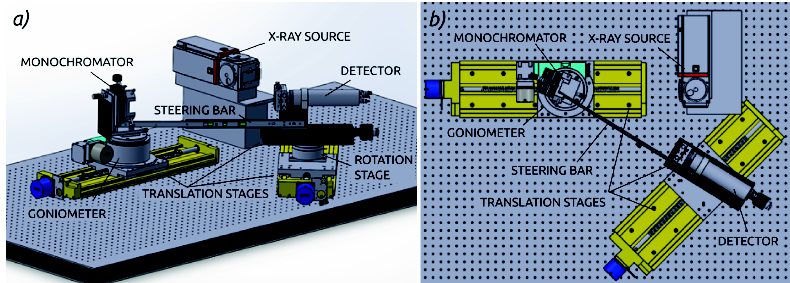
\includegraphics[width=\textwidth]{../Kuvat/cad_setup.png}
  \caption{3D model of the HelXAS setup.}
  \label{fig:cad}
\end{figure} 

The monochromator crystal is installed on top of a Huber goniometer, which controls the Bragg's angle $\theta_B$. The crystal goniometer installation is placed on a linear stage, which controls the distance between source and monochoromator noted as $\rho$. The $\rho$ is related to $\theta_B$ as $\rho = R_bsin\theta_B$, where $R_b$ is the bending radius of monochromator crystal.  

Motors and data acquisition is run on SPEC version 6 by Certified Scientific Software.   

\subsection{Preparations for Anaerobic Samples}
For the anaerobic samples we had to design a new sample environment. In our design the sample is placed between two $\SI{0.1}{\milli\metre}$ kapton foils, and sealed with $\SI{1}{\milli\metre}$ thick o-ring. This setup is compressed by two aluminium plates and eight screws. The window on the aluminium plates has a diameter of $\SI{10}{\milli\metre}$, and there are 8 slots for samples. The design is show in figure \ref{fig:n�ytteenvaihtaja}.

\begin{figure}[h!]
  \centering
    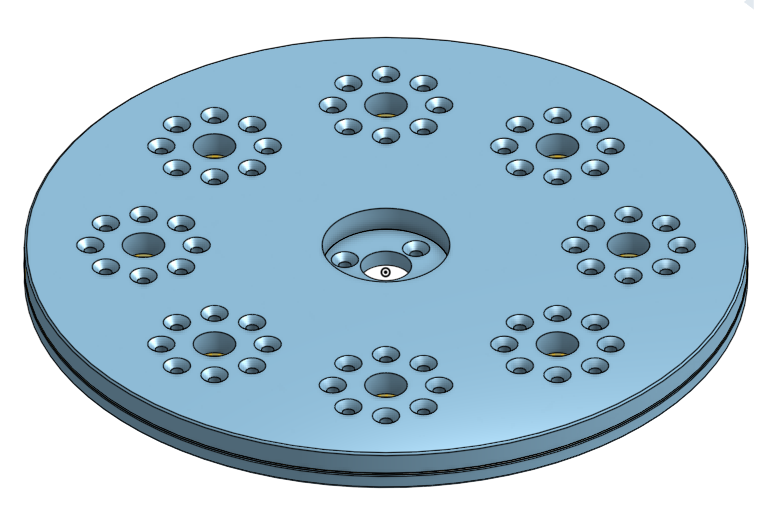
\includegraphics[width=0.7\textwidth]{../Kuvat/vaihtaja.png}
  \caption{The design of the anaerobic chambers.}
  \label{fig:n�ytteenvaihtaja}
\end{figure}
The sample plate is motorized, which allows us to automate the measurements.

\subsection{Background Noise}
When performing the measurement, the background noise is always present. Background noise is caused by elastic scattering, fluorescence, etc. Since the $\mu x$ is obtained from a logarithm, it is highly non-linear, and thus sensitive to background noise. 

The background noise can be taken into account by measuring it by moving the detector away from the direct beam. The accuracy of background measurement can be improved by measuring the background from both sides of the beam and taking the mean. The background is slowly varying, so in order to avoid statistical noise, a low order polynomial is fitted and the fit is removed from the signal.    

\subsection{Measurement Procedure}
First we measure the direct beam $I_0$ and the transmitted beam $I$ and their backgrounds $I_{0,bg}$ and $I_{bg}$. Then we apply the dead time correction from equation \ref{eq:deadtime}. Next we fit low order polynomials $y$ and $y_0$ to the backgrounds $I_{0,bg}$ and $I_{bg}$. Finally we compute the $\mu x$ from equation

\begin{equation} \label{eq:mux}
\mu  x=\ln\frac{I_0-y_0}{I-y}.
\end{equation}


\chapter{Preparation of Soil and Brackish Water Samples}\label{preparation}
\section{Reference Samples}\label{ref}
In order to estimate the chemical state of our system, we acquired a set of reference samples of some well known \ch{Fe} compounds. These samples can be used as a fingerprint for each compound and allow us keep track of the chemical state of our soil samples. In all of our  measurements we used $\SI{0.01}{\milli\metre}$ iron foil to keep track of our energy calibration. 
\section{Soil and Brackish Water Samples}\label{samples}
\subsection{Soil Samples}
The soil we received was obtained from five different locations. The soil was weighted by using a scale with an accuracy of $10^{-4} \si{\gram}$. The soil was then mixed with farina in approximately 1:4 concentration. After mixing we added some ethanol and ground using a mortar until the ethanol was evaporated. The result was a fine mix with a uniformly small particles. The mix was then placed in a M5 washer and sealed with Scotch tape. From the five different soils we made two samples of each.  
\subsection{Soil and Brackish Water Jellys}
The measurement of wet samples turned out to be trickier than expected. When the sample was placed in front of the X-ray tube, the bremsstrahlung, caused by the x-ray and sample atom interaction, broke the bonds in the water molecules. The broken water molecules released \ch{O}-radicals, which interacted with our samples and after few hours most of the water molecules broken, causing the sample to look like a dry soil, and the chemical state of the sample was altered.

Second problem we encountered was the sample heterogeneity. When the soil is mixed with water, it tends to sediment. The sedimentation causes soil to accumulate at the bottom of the sample environment. Also when the sample is rotated, the smaller particles move faster and larger particles/clusters may stay still. Now when placing the sample in front of the detector and scanning the energy range by changing the angle $\theta$, we might hit just the water or the soil with different thickness or particle size. 

In order to tackle the problems stated above we decided to do two things. The first one was to place the sample in front of the detector to reduce the amount of photons interacting with our sample. The second one was to make gel of our samples with agar. We took the water where the samples were mixed in, and added approximately $1-0.5$ $wt\%$ of agar. The water was then heated to boiling and mixed all the time with magnetic stirrer. Heating was turned off when the water reached boiling temperature and the sediment was mixed with water after the water reached approximately $60\si{\celsius}$. The mix was then quickly placed in the sample environment and cooled in a fridge. This method allowed us to make homogeneous samples to be placed in front of the detector. 

We tested the optimal water/soil ratio for our samples by mixing soil and water in ratios 1:4, 1:8 and 1:16. We then measured the absorption spectra of these mixes \ref{fig:jellytest}.
\begin{figure}[h!]
   \centering
     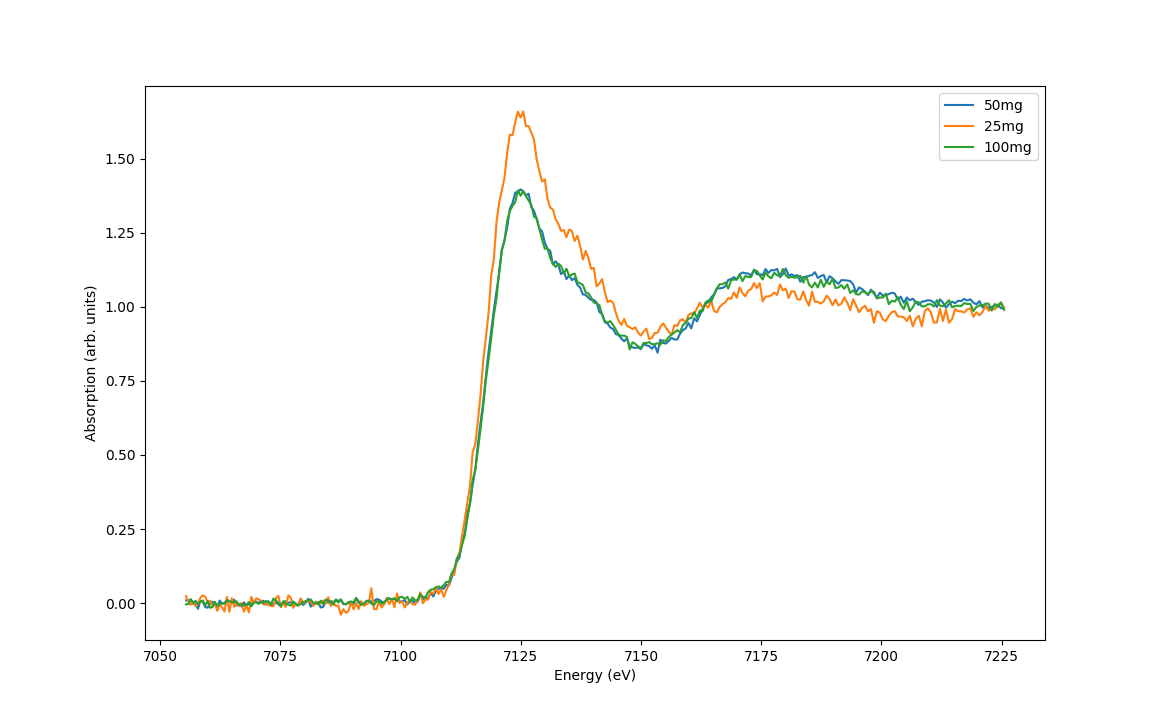
\includegraphics[width=\textwidth]{../Kuvat/JellyTest.png}
   \caption{The x-ray absorption spectra different gel mixes.}
   \label{fig:jellytest}
\end{figure}
As a result for this test we concluded that we need high enough soil/water concentration to make the normalization of our spectra easier. 
\subsection{Anaerobic Soil and Brackish Water Jellys}
The sample preparation of anaerobic wet samples was rather similar to the preparation of our normal wet samples. The major difference was that the sample preparation was done in \ch{N2} atmosphere. We used an anaerobic chamber found in Viikki campus of University of Helsinki, shown in figure \ref{fig:kaappi}, for our sample preparation. The \ch{N2} atmosphere was pressurised, which made  weighing the agar rather complicated task. With most of the samples the $wt\%$ of agar was not accurate, and the amount of agar had to be estimated with approximately. The temperature in the anaerobic chamber was circulating around $30^\circ$C so we used ice and copper rods to cool the sample instead of fridge.

\begin{figure}[h!]
   \centering
      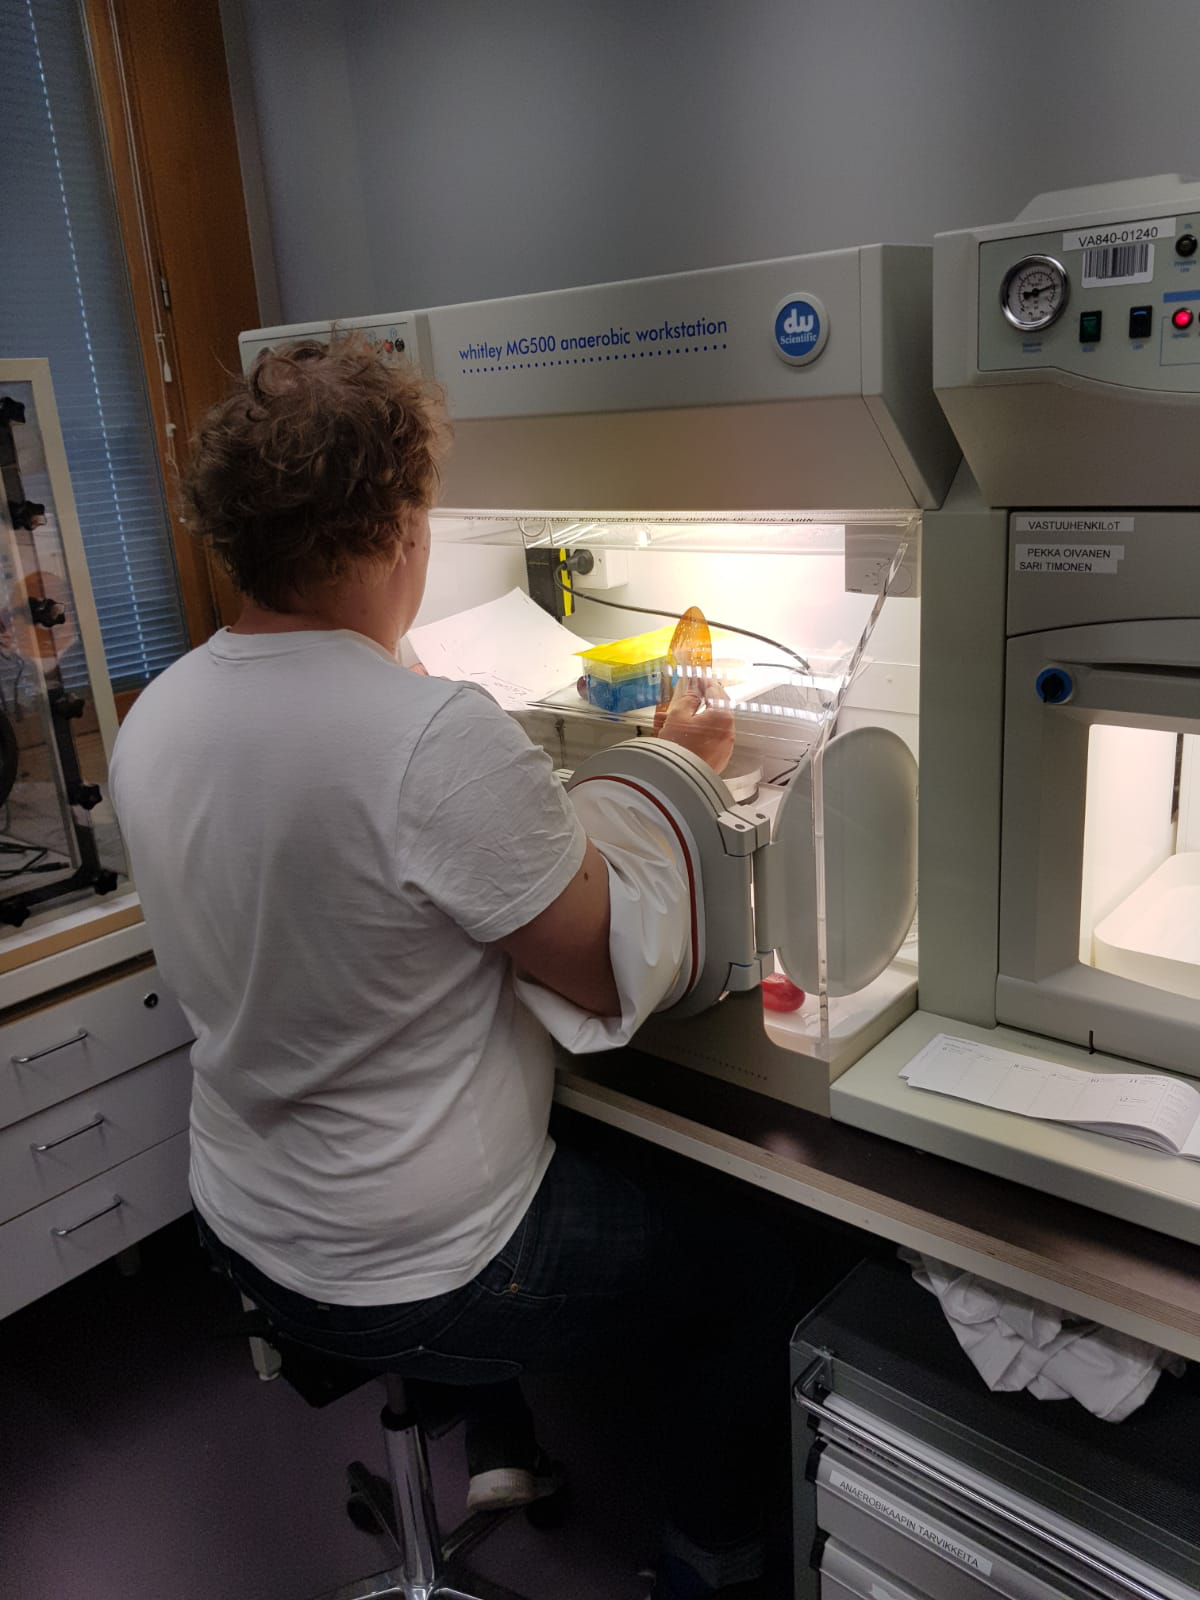
\includegraphics[width=0.6\textwidth]{../Kuvat/kaappi.png}
   \caption{The anaerobic chamber in Viikki campus.}
   \label{fig:kaappi}
\end{figure} 

Even with these constrains the sample preparation was rather straight forward and we managed to produce smooth homogeneous jelly. The samples endured the measurement and the black color on samples with \ch{C} treatment, indicating the presence of sulfides, lasted until the sample environment was opened after the measurement.     

\subsection{The Effects of Agar}
In order to eliminate the radiation damage in water molecules, we decided to turn the water into a gel. This also helped us to achieve proper sample uniformity as the soil particles were "frozen" in place in the gel. The agar we used was powder for bacteriology from WVR chemicals \cite{Vwr}. Our Agar had a melting point at $90\si{\celsius}$ and gelling point at $30-40\si{\celsius}$. This meant that we didn't need to boil our water, and when we mixed the water with soil, the temperature of the soil never increased over $50\si{\celsius}$. The changes in \ch{Fe} chemistry happen mainly through redox reactions \cite{Agar}, and since we only heat the sample for a relatively short time period to a modest level, we can expect that the heating will not cause any changes in the chemical state. 

As for the added agar, as it turns into a gel, it forms a double helical structure. By joining double helices, three-dimensional structure framework is formed, which holds water molecules within interstices of the framework \cite{Agar}. Agar gel is rather stable under normal laboratory conditions. Exposure to extended periods of high temperatures and pHs lower than 6.0 can lower gel strength. These conditions can be easily avoided during our experiments. The main concern is that agar-gel is fertile media for bacteria, and in room temperatures we might see growth of micro-organisms. However we are able to perform our measurement within $10-14 \si{\hour}$ after the gel formation, and during that time period, the bacteria growth should still be relatively minimal. Typically visible bacteria growth is seen after 2-3 days \cite{Agar}.
\chapter{Results and Discussion}\label{tulokset}
\section{Analysis}
\subsection{Data Reduction}
The measured data represents the incoming photons per measurement time in each angle step. In order to gain access to the absorption coefficient as a function of energy, we use the following steps:
\begin{enumerate}
\item The measured intensities are converted to $\mu(E)$, by using the equation \ref{eq:beer}.
\item A smooth line is fitted to the pre-edge region of the spectrum and then subtracted from the $\mu(E)$ in order to get rid of the instrumental background and absorption from other edges.
\item The threshold energy $E_0$ is identified as the maximum derivative of $\mu(E)$.
\item $\mu(E)$ is normalized from 0 to 1.
\end{enumerate}
\subsection{Curve Fitting to Reference Samples and Measurements}
To approximate how much of a certain component was formed during the incubations, we needed to compare the result with known reference samples. Since we are comparing the initial state with a final state, in which we expect a new component, we can try to match the final state by performing a least squares linear combination fitting. This allows us to quantify the different species in multi-component mixtures from their XANES 
fingerprints. Least squares algorithm refine the sum of a given number of reference spectra to an experimental spectrum. The reference compounds need to be recorded under similar conditions, and one needs good quality data. 

In least squares we minimize the sum, $S$, of squares residuals 

\begin{equation}
S=\sum_{i=1}^n r_i^2
\end{equation}
where $r_i$ is the difference between observed value $y_i$ and the fitted value $f(x_i,\beta)$, also know as residual:  
\begin{equation}
r_i=y_i-f(x_i,\beta).
\end{equation}
The fitted value $f(x_i,\beta)$ is based on vector $\beta$, which holds $m$ adjustable parameters, and on the independent variable $x_i$. The goal of this method is to find parameter values which make the model function represent measured data most accurately. The variance is obtained with 
\begin{equation}
\sigma^2=\frac{1}{n-p}S,
\end{equation} 
where $n$ is the number of observations and $p$ the number of variables.

Sometimes the quirkiness of the measurement can cause problems with least squares. The error-bars might be rather small, and some of the data points do not fit inside of those. These so-called outlier points have to be taken into account. We are using the Couchy formulation to address this issue \cite{Data}. In Couchy formulation the uncertainties are assumed to be of the same order as in the standard least squares, which we note as $\sigma_0$, but they can be either smaller or larger. The prior in this case is proportional to $\exp{(-\sigma_0/\sigma)/\sigma^2}$. Whit this method we use the same model function and the initial guess for the parameters $\beta$ to obtain a likelihood function: 

\begin{equation}
L=\sum\ln\Big(\frac{1-e^{-R^2/2}}{R^2}\Big)
\end{equation}
where the $R$ has the following form: 
\begin{equation}
R=\frac{f(x,\beta)-y}{\sigma_0}.
\end{equation}
By maximizing the likelihood and uncertainty $\sigma$, we are able obtain more accurate results.

 The uncertainty $\sigma$ in this case is only based on the variance in the data, and doesn't take into account physical error sources. One source of systematic error is that our \ch{FeS} reference doesn't fully represent new chemical species, since we might have other components, such as pyretite (\ch{FeS2}), present in the final state. We will however represent $\sigma$ along our fit results, but it is to be taken with grain of salt.   
 
\section{Measurement results}
\subsection{Dry Soil Samples}
Each of the soil was measures four times between Bragg angles $\theta_{min}=68.5^{\circ}$ and $\theta_{max}=72.5^{\circ}$, the range was divided into 300 measurement points, and the intensity was measured for $5$ seconds in each point.  All the soil samples had relatively similar spectra (\ref{fig:drySoil}). The samples were collected from similar height from the sea level, and from a restricted geographical area, so their geological age and other properties should be relatively similar.
\begin{figure}[h!]
  \centering
    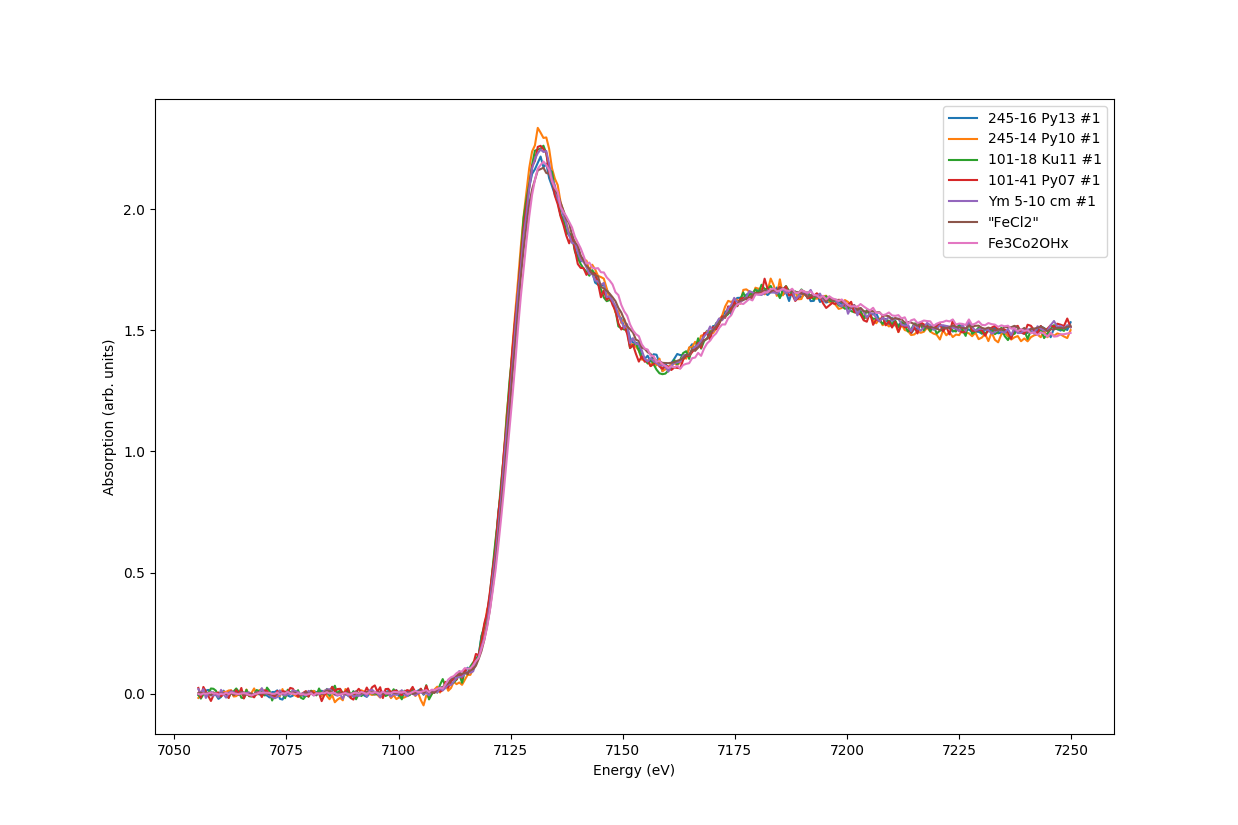
\includegraphics[width=\textwidth]{../Kuvat/Dry_Soil_Samples1.png}
  \caption{The spectra of dry soils.}
  \label{fig:drySoil}
\end{figure}

Our measurement of dry soil samples produced the expected results and the spectra were very similar with different iron hydroxides. Iron hydroxides, for example ferrihydrate and goethite, have very similar spectra with each other, so with XANES it is difficult to evaluate the exact chemical species. However we can state that the iron in the samples is present mainly as \ch{Fe}(III) hydroxides. The spectra might consist of multiple different \ch{Fe} hydroxides and in order to fully obtain knowledge of the components, some other characterisation technique should be used. We can use this result as a fingerprint of the initial chemical state of our system.  

We also made another sample from each of the soils to test the homogeneity of our soils. The results are shown in figure \ref{fig:dryHomogenity}, and  is clearly visible, the samples are very homogeneous. 

\begin{figure}[h!]
  \centering
    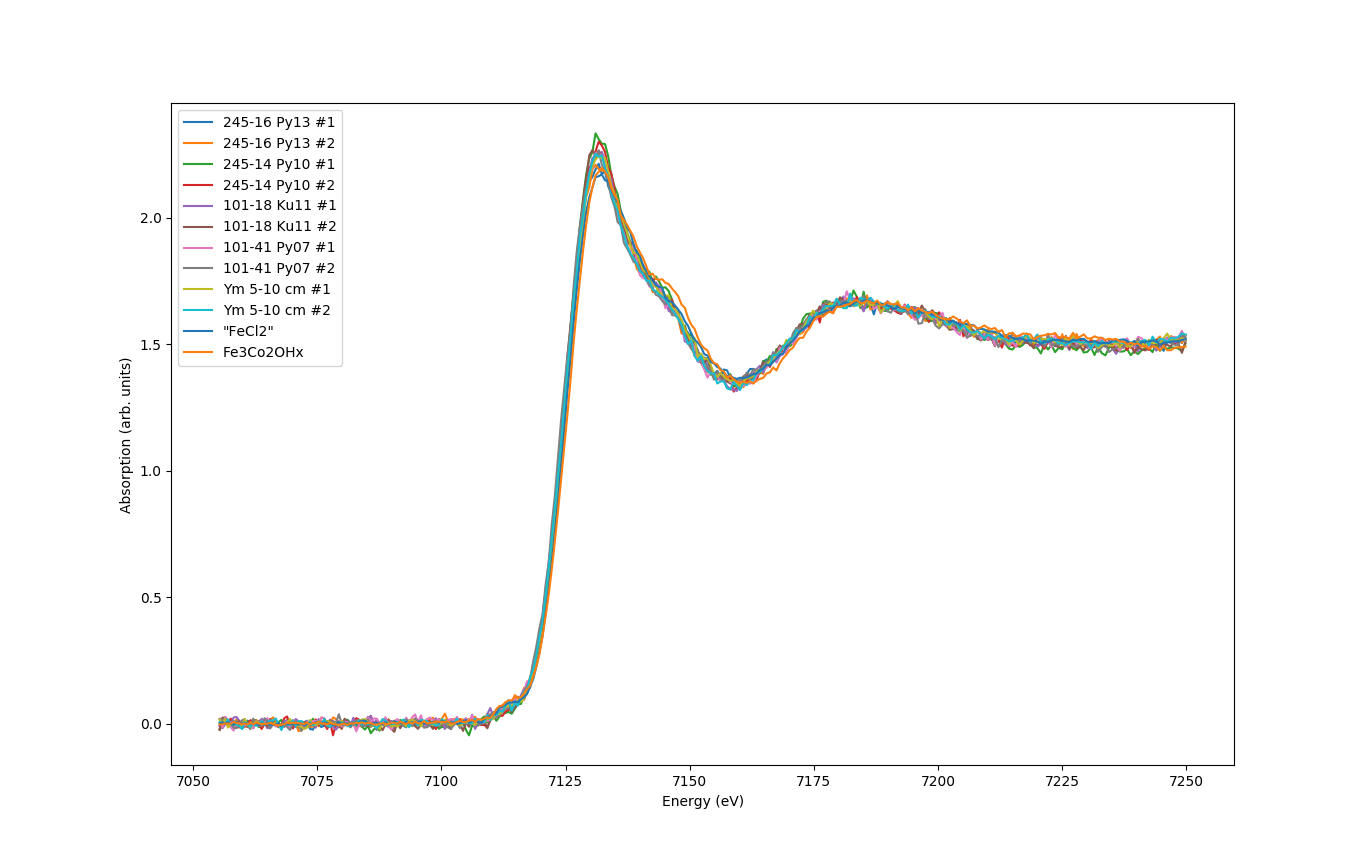
\includegraphics[width=\textwidth]{../Kuvat/dry_soil_samples_all.png}
  \caption{The spectra of all dry soils.}
  \label{fig:dryHomogenity}
\end{figure}

\subsection{Wet Samples After 24 Hours}
The soils were then placed in glass bottles for incubations. Sea water was added and the bottles were placed in a temperature of $\SI{5}{\celsius}$ and in a dark environment. The notation of the samples was also changed in comparison with the dry samples, and is shown in table \ref{tab:wet}. The order from 1 to 5 was based on \ch{Fe} oxide levels, 1 having the most and 5 the least. In order to simulate effects of organic \ch{C} and increased \ch{SO4} levels we used sodium acetate (\ch{CH3COONa}) and potassium sulfate (\ch{K2SO4}) in our incubations. This allowed us to form a set of samples in a binary fashion shown in figure \ref{tab:wet}. Since the main focus of this work was the cases with added \ch{SO4}, we made samples with no added \ch{SO4} only from M1 and M5 soils. The samples were collected from these bottles after 24 hours, and then made into a gel.

\begin{table}[]
\centering
\begin{tabular}{|l|l|l|l|l|l|}
\hline
Soil & Dry  notation & C0S1 & C1S1 & C0S0 & C1S0 \\ \hline
M1   & Ym 5-10 cm    & x    & x    & x    & x    \\ \hline
M2   & 245-16 Py 13  & x    & x    & -    & -    \\ \hline
M3   & 101-18 Ku 11  & x    & x    & -    & -    \\ \hline
M4   & 245-14 Py 10  & x    & x    & -    & -    \\ \hline
M5   & 101-41 Py 07  & x    & x    & x    & x    \\ \hline
\end{tabular}
\caption{A summary of prepared samples.}
\label{tab:wet}
\end{table}
 
We now had to place the sample in front of the detector, in order to avoid radiation damage. This reduces the amount photons hitting our sample. With the added water we expect the chemical state to remain the same with the dry samples, since the mineralization process takes several weeks to take place. The measurement result for C1S1 samples is shown in figure \ref{fig:wetsoil}. C0S1, C0S0, C1S0 samples can be found from appendices in figures \ref{fig:wetsoilC} and \ref{fig:wetsoil_others}.

\begin{figure}[h!]
  \centering
     \centerline{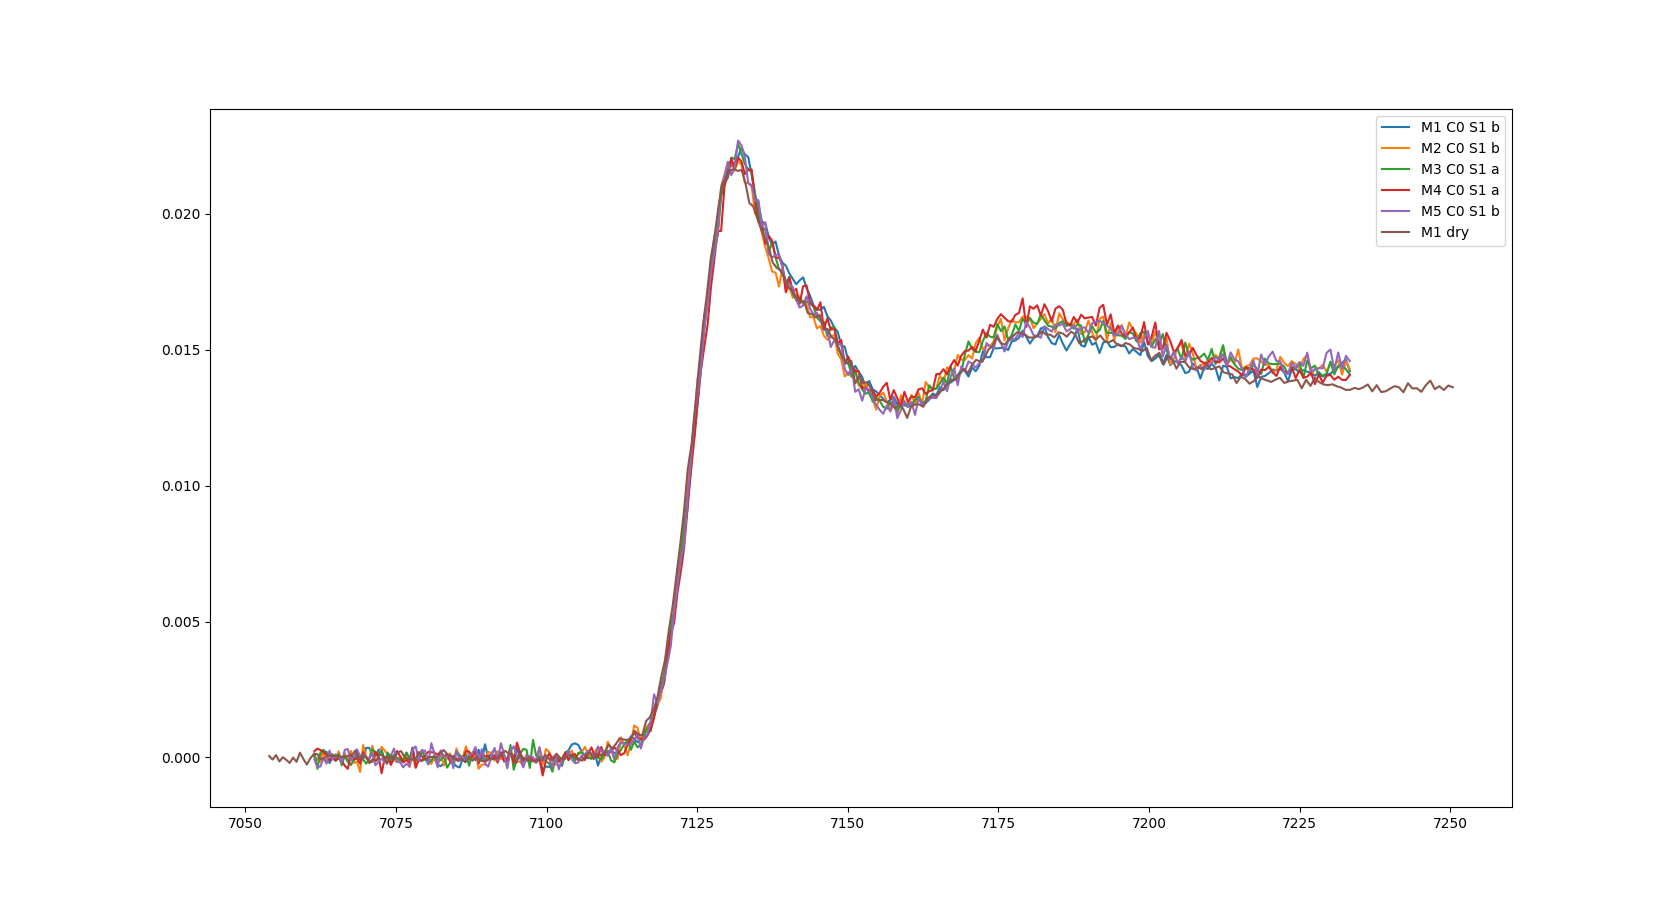
\includegraphics[width=1.3\textwidth]{../Kuvat/Sulfideja/wetC2.png}}
  \caption{The spectra of wet samples with added \ch{C} after 24 hours of incubation.}
  \label{fig:wetsoil}
\end{figure}

The chemical state seems to remain the same in all of our measurements. Two of the samples, M1C0S0b and M5C1S1b, have slightly different height in the white line region. This is probably caused by small water/soil ratio in the sample, which we discussed in the sample preparation section. The peaks, valleys and other spectral features in these two samples seem to happen at similar energies compared to other samples, so the chemical state can be expected to remain the same as in the other samples. We collected our samples from larger bottles, and some of them had very small amounts of water or soil, which made the sample preparation more difficult. In the next sampling we addressed this issue by taking larger amounts of both soil and water from the larger bottles.   

\subsection{Anaerobic Wet Samples}
We improved our measurement by splitting it into three parts. In the first 75 measurement points we used 1 second measurement time, in the next 135 measurement points 15 seconds and in the last 90 points again 1 second. This allowed us to get better quality data from the sections where we see the largest changes in the spectra in case of altered chemical state.
\subsubsection{Samples with no added Carbon}
In case of no added \ch{C} the samples were incubated in $5\si{\celsius}$ in a dark room for two months. After two months the samples looked visually the same as after two days. XAS results however revealed an altered chemical state. The measurement result for M4 soil is represented in figure \ref{fig:M4_noC}. Other measurements can be found in appendices in figures \ref{fig:M1_noC}, \ref{fig:M2_noC}, \ref{fig:M3_noC} and \ref{fig:M5_noC}. Our results showed that no sulphides were formed and no  \ch{Fe2O3} were formed either. It is clear that there is no obvious shift in the rising edge, and thus the oxidation state has approximately remained the same. However small amounts of species with a different oxidation state might be difficult to detect.  
%\begin{figure}[h!]
%  \centering
%    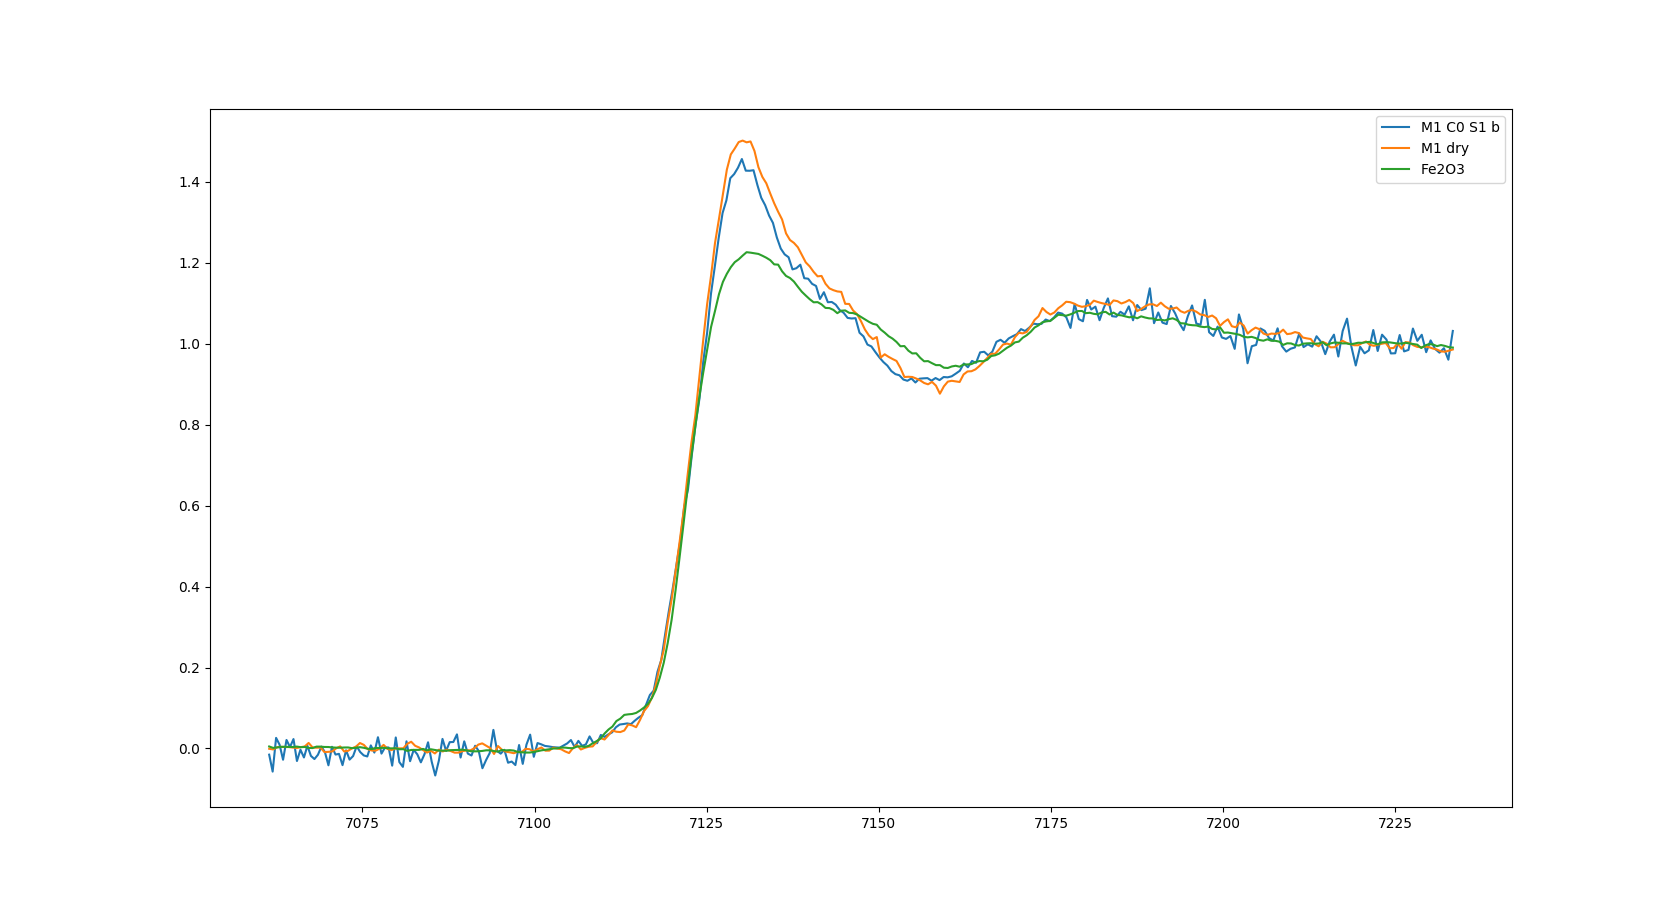
\includegraphics[width=0.9\textwidth]{../Kuvat/Sulfideja/M1_Fe2O3.png}
%  \caption{M1 soil with no added \ch{C} after two months of incubation. The results are compared to the dry sample and \ch{Fe2O3} reference sample.}
%  \label{fig:M1_noC}
%\end{figure}

%\begin{figure}[h!]
%  \centering
%    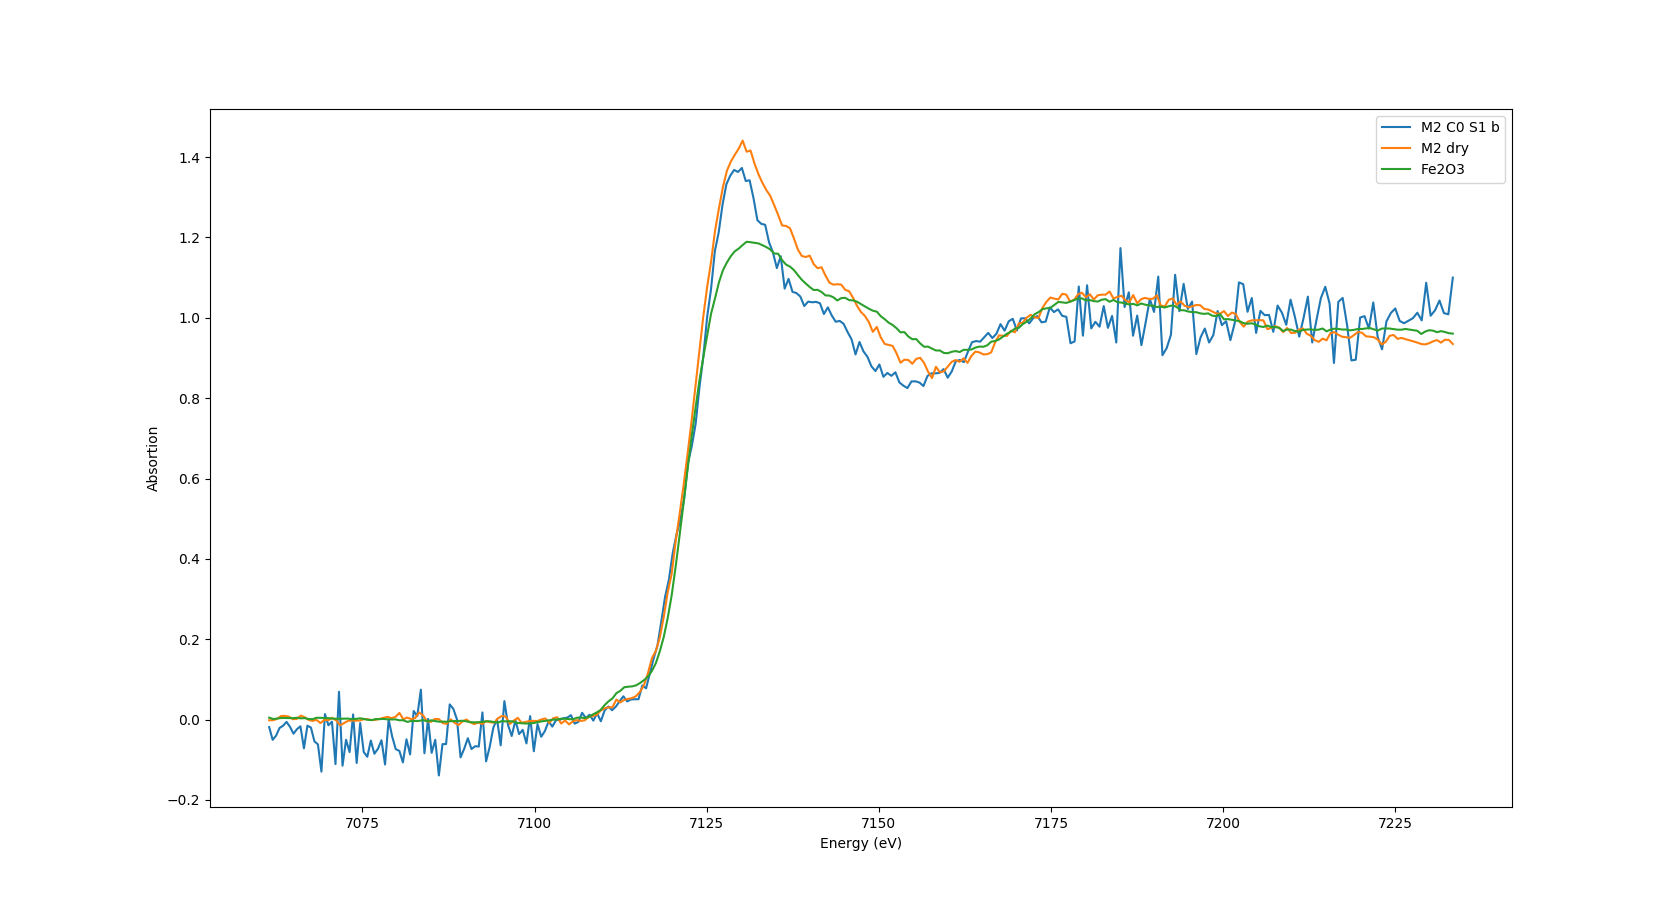
\includegraphics[width=0.9\textwidth]{../Kuvat/Sulfideja/M2_Fe2O3.png}
%  \caption{M2 soil with no added \ch{C} after two months of incubation. The results are compared to the dry sample and \ch{Fe2O3} reference sample.}
%  \label{fig:M2_noC}
%\end{figure}

%\begin{figure}[h!]
%  \centering
%    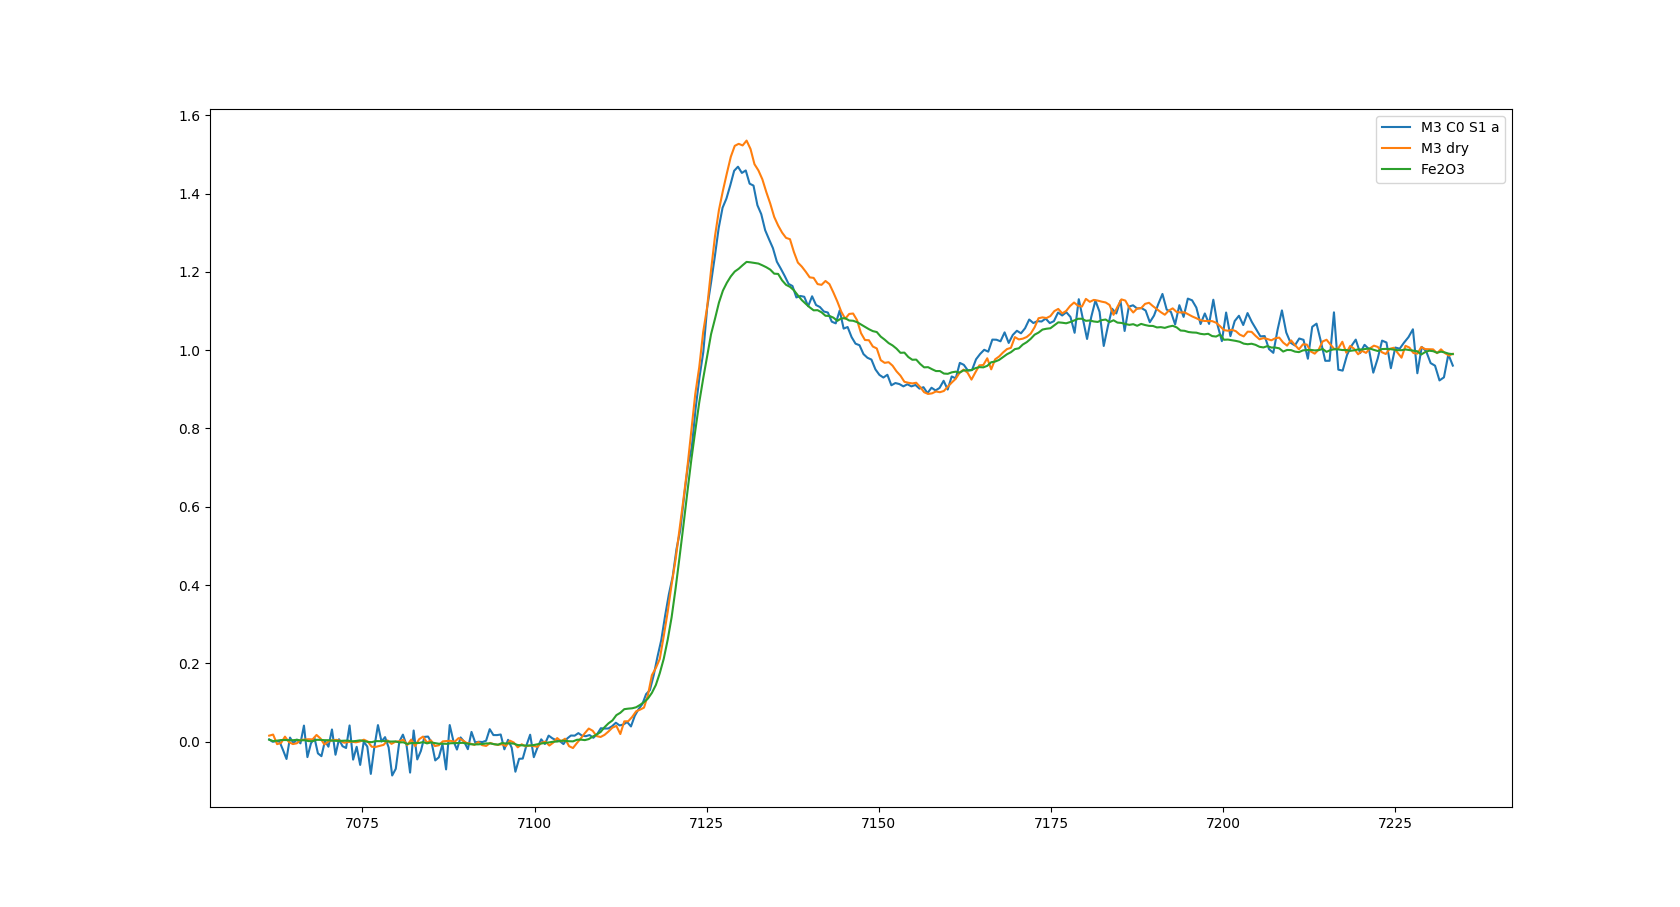
\includegraphics[width=0.9\textwidth]{../Kuvat/Sulfideja/M3_Fe2O3.png}
%  \caption{M3 soil with no added \ch{C} after two months of incubation. The results are compared to the dry sample and \ch{Fe2O3} reference sample.}
%  \label{fig:M3_noC}
%\end{figure}

\begin{figure}[htb!]
  \centering
    \centerline{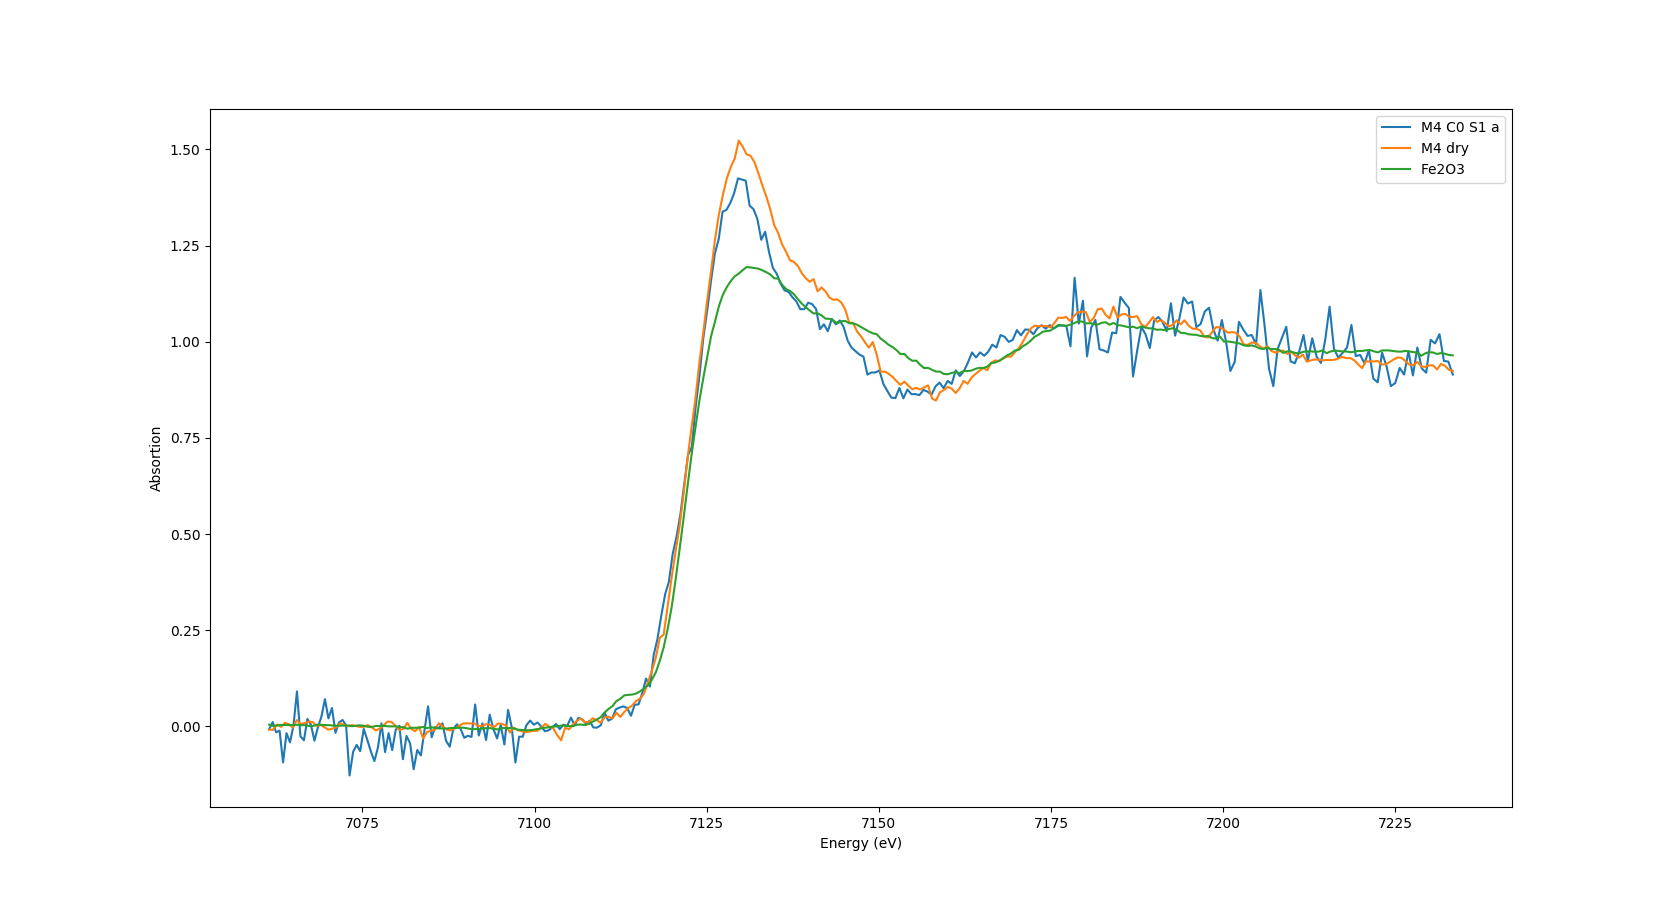
\includegraphics[width=1.3\textwidth]{../Kuvat/Sulfideja/M4_Fe2O3.png}}
  \caption{M4 soil with no added \ch{C} after two months of incubation. The results are compared to the dry sample and \ch{Fe2O3} reference sample.}
  \label{fig:M4_noC}
\end{figure}

%\begin{figure}[h!]
%  \centering
%    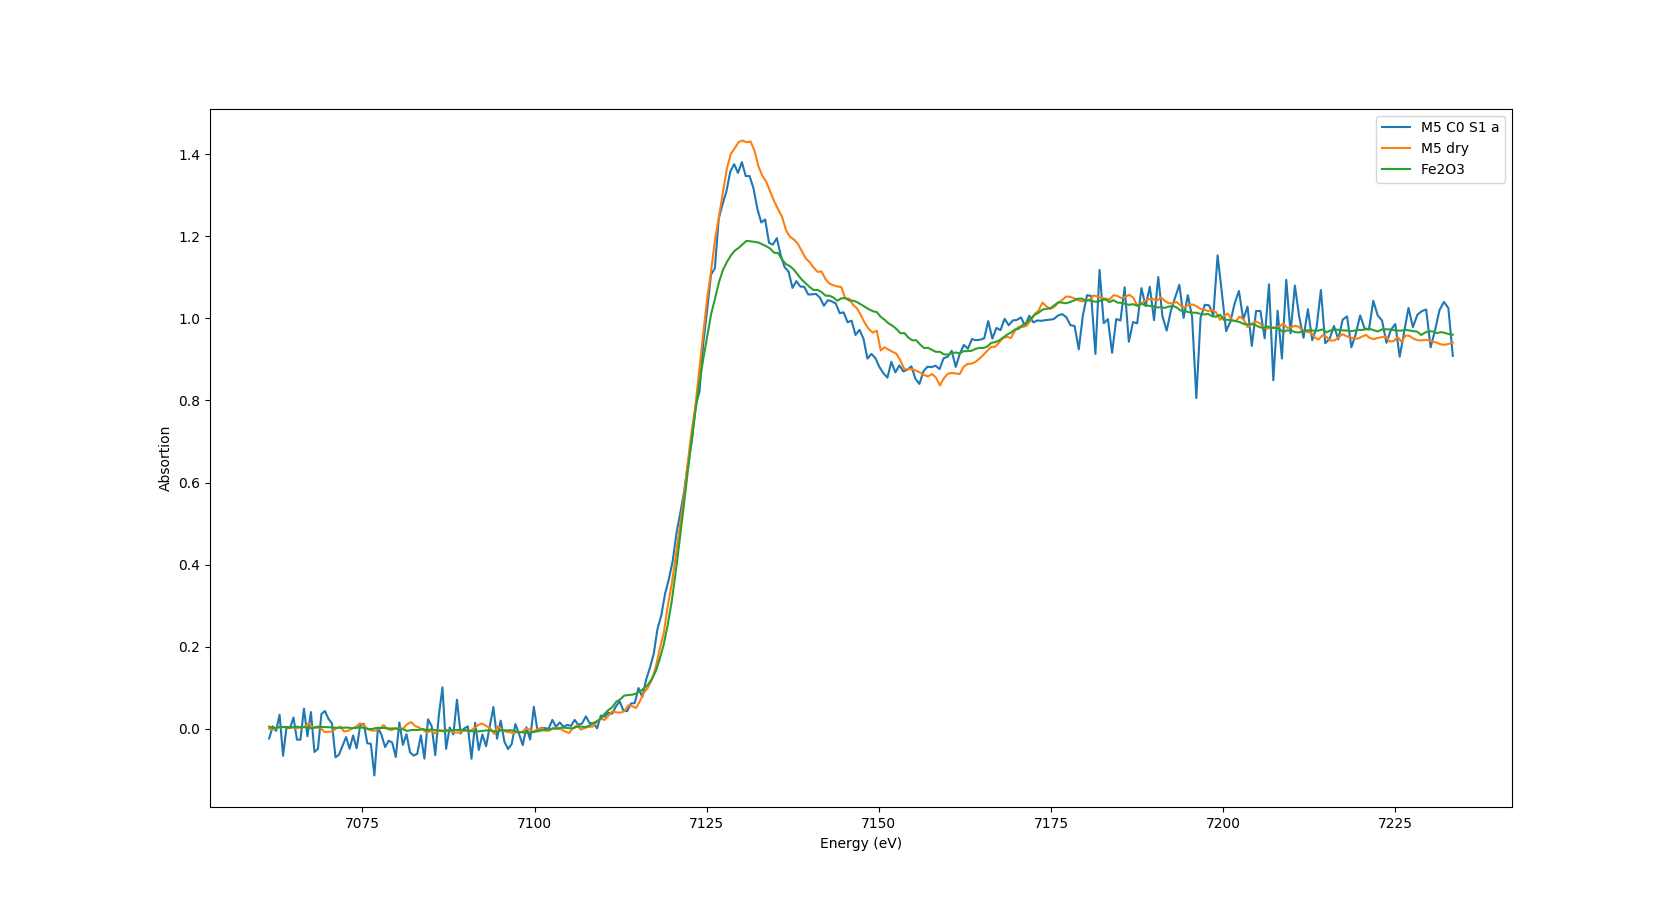
\includegraphics[width=0.9\textwidth]{../Kuvat/Sulfideja/M5_noC.png}
%  \caption{M5 soil with no added \ch{C} after two months of incubation. The results are compared to the dry sample and \ch{Fe2O3} reference sample.}
%  \label{fig:M5_noC}
%\end{figure}

To gain better understanding of this result we performed a simulation of certain \ch{Fe} complexes. We used FDMNES software \cite{FDMNES} for these simulations, and the results are shown in figure \ref{fig:simu}.

\begin{figure}[htb!]
  \centering
     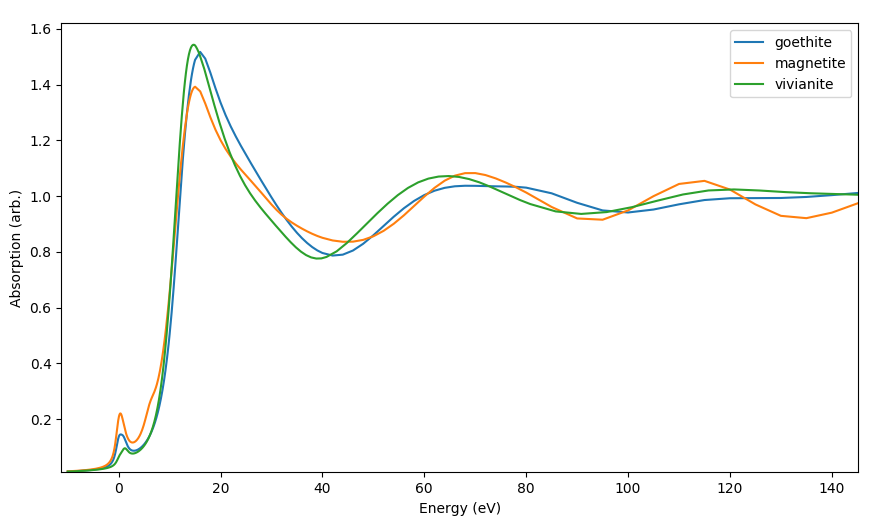
\includegraphics[width=0.8\textwidth]{../Kuvat/mineral_spectra.png}
  \caption{Simulation results of our FDMNES simulation of a few \ch{Fe} minerals.}
  \label{fig:simu}  
\end{figure} 
The simulation results indicate, that the new component present in our measurements is vivianite. Unfortunately we were not able to acquire unoxidised vivianite to be used as a reference for our measurements. In the literature we found one measurement, where both \ch{FeS} and vivianite were measured by Sulu-Gambari F. et al. \cite{VivSpectra}. Their results are shown in figure \ref{fig:Sulu}.
\begin{figure}[htb!]
  \centering
     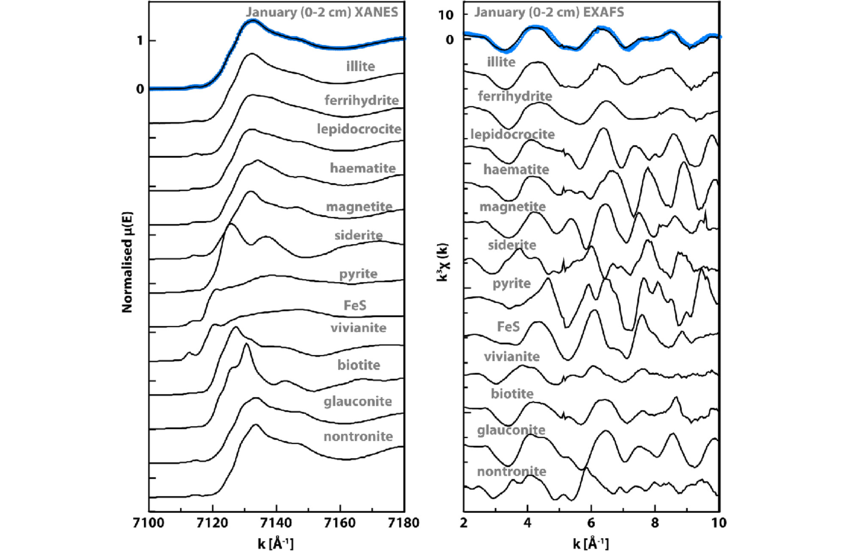
\includegraphics[width=0.8\textwidth]{../Kuvat/vivianiitti_spectra.png}
  \caption{The measurement results of Fe K-XANES of certain Fe minerals from the literature \cite{VivSpectra}.}
  \label{fig:Sulu}
\end{figure}
These were measurements of their so called reference samples, and they did not specify was the sample oxidized or not. This makes the comparison with our samples difficult, since we want be to sure that the vivianite is unoxidized. 

Another possible explanation is that \ch{PO4} has bonded in some other way with \ch{Fe} minerals. For example Khare et al. have studied the bonding of \ch{PO4} with ferrihydrite \cite{KHARE20074405} and proposed bonding shown in figure \ref{fig:po4}.

\begin{figure}[htb!]
   \centering
     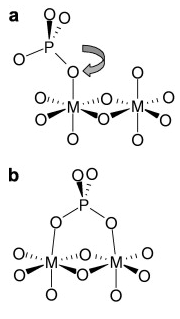
\includegraphics[width=0.3\textwidth]{../Kuvat/FePo.png}
   \caption{Drawing of the idealized metal phosphate complexes utilized in Extended-H�ckel calculations for (a) monodentate and (b) bidentate coordination \cite{KHARE20074405}.}
   \label{fig:po4}   
\end{figure} 
This problem has to be tackled in future measurements, and we probably have to make the unoxidized vivianite sample chemically in anaerobic environment, along with other iron oxyhydroxides.  
     
\subsubsection{Samples with added Carbon}
Similarly the samples with added \ch{C} were also incubated in a cold and dark room for two months. The color of the soil was altered into black, which indicated that sulphides had been produced. The results for M4 soil is shown figure \ref{fig:M4_C}. Other measurement results can be found from appendices in figures \ref{fig:M1_C},\ref{fig:M2_C} and \ref{fig:M5_C}.

%\begin{figure}[!htb]
%  \centering
%    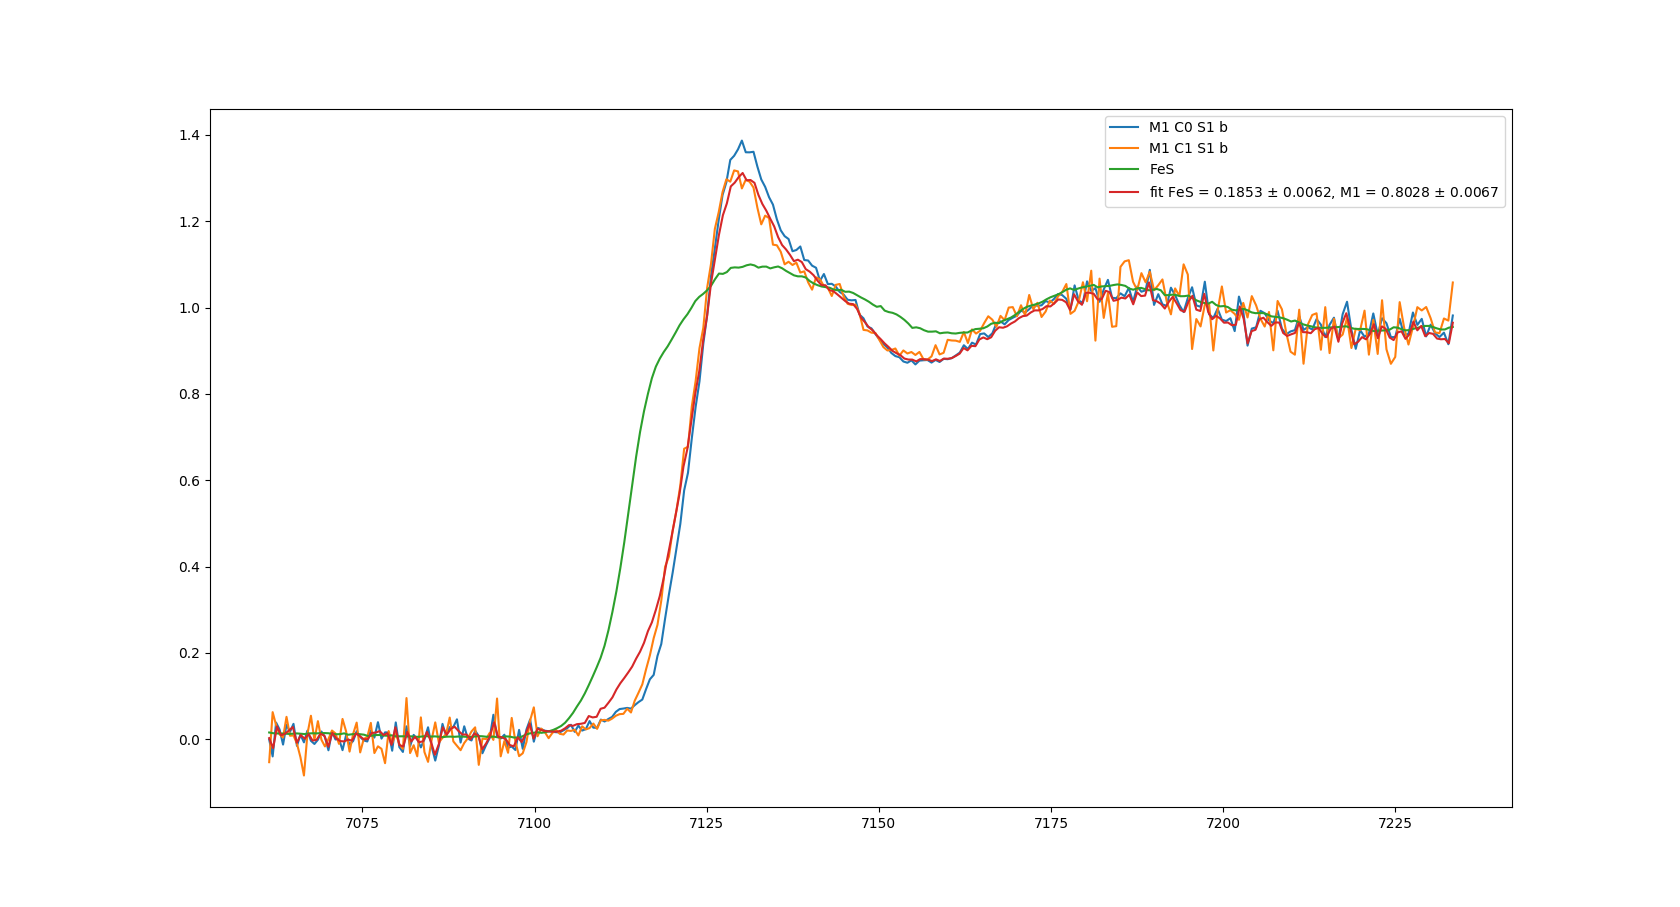
\includegraphics[width=0.9\textwidth]{../Kuvat/Sulfideja/M1_cauchy.png}
%  \caption{M1 soil with added \ch{C} after two months of incubation, compared with \ch{FeS} reference and the case with no added \ch{C}}
%  \label{fig:M1_C}
%\end{figure}

%\begin{figure}[!htb]
%  \centering
%    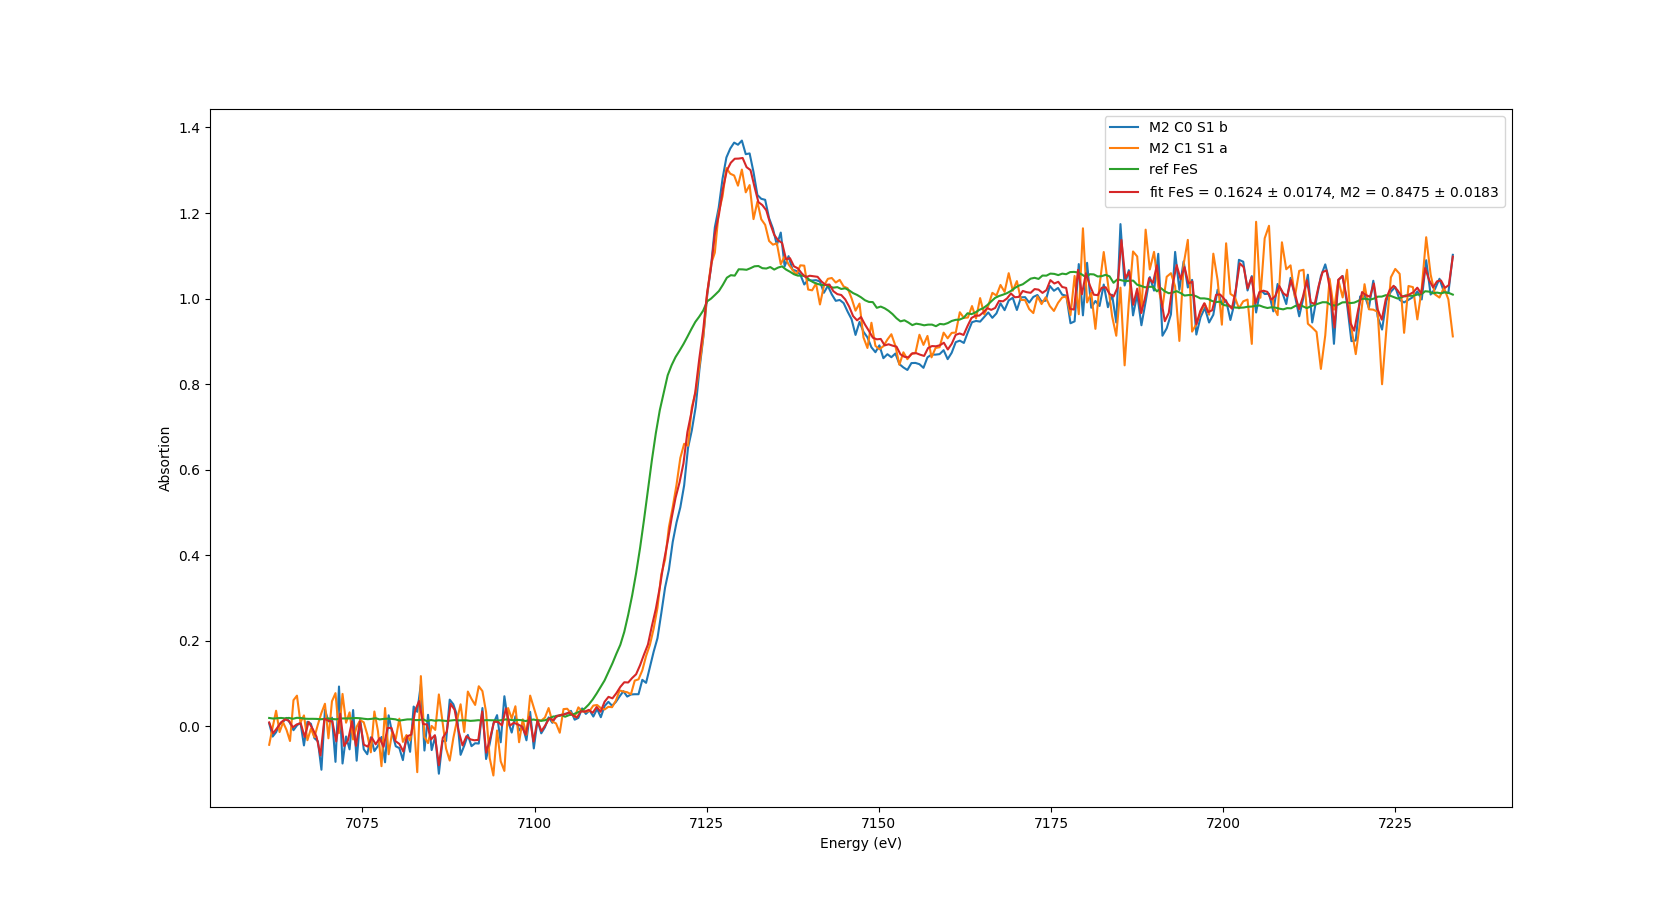
\includegraphics[width=0.9\textwidth]{../Kuvat/Sulfideja/M2_cauchy.png}
%  \caption{M2 soil with added \ch{C} after two months of incubation, compared with \ch{FeS} reference and the case with no added \ch{C}.}
%  \label{fig:M2_C}
%\end{figure}

\begin{figure}[!htb]
  \centering
    \centerline{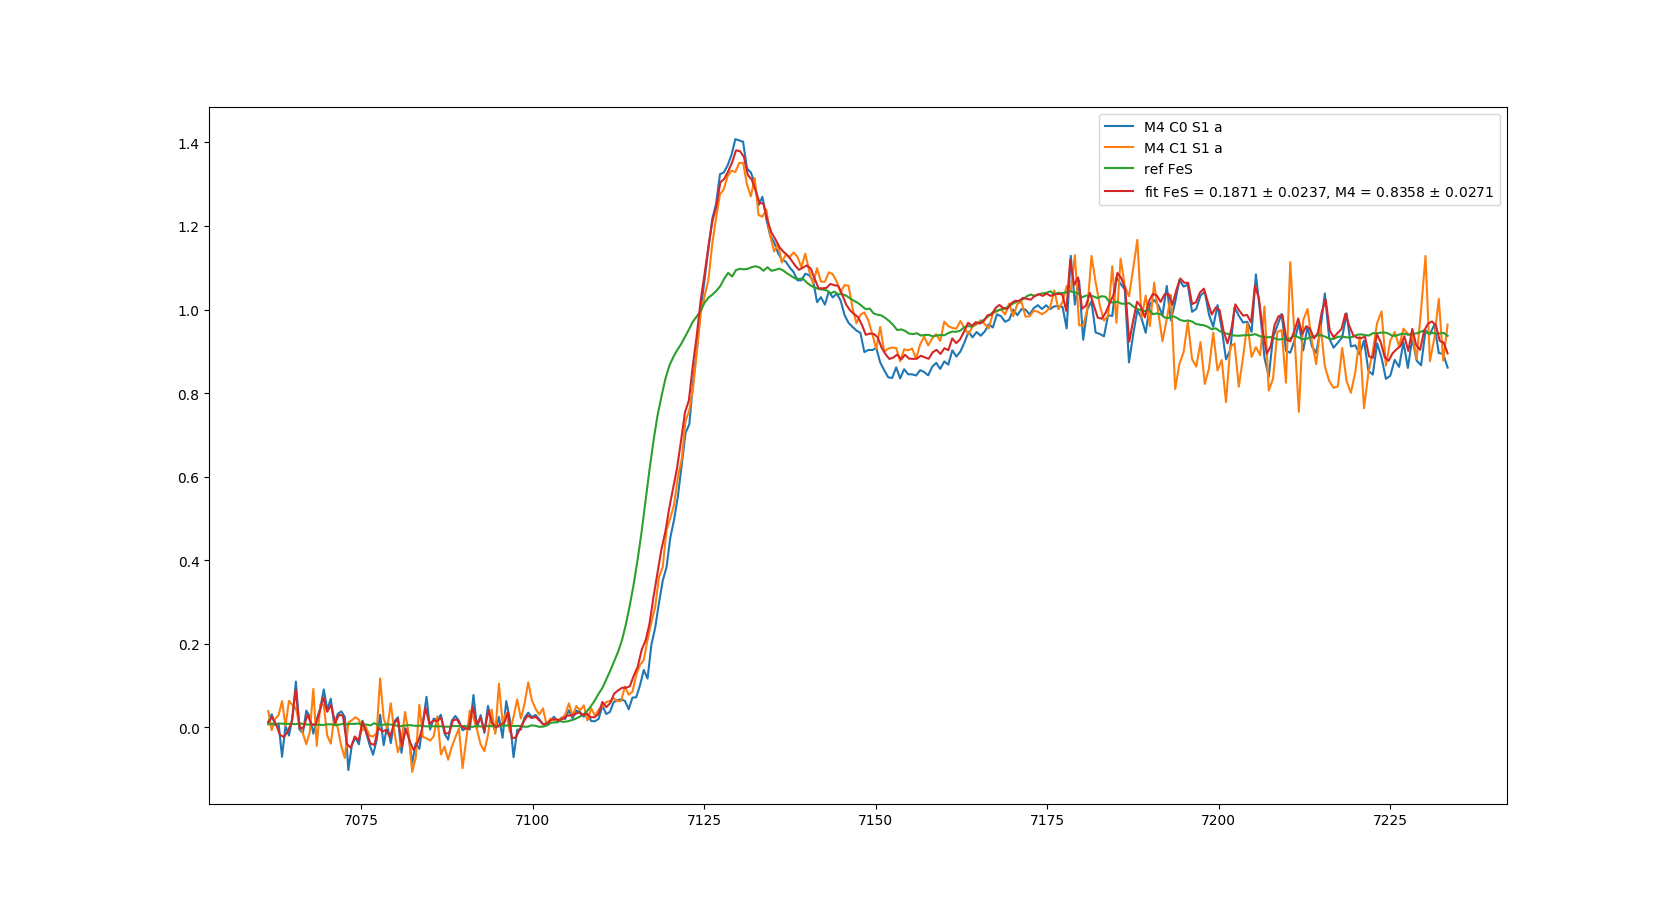
\includegraphics[width=1.3\textwidth]{../Kuvat/Sulfideja/M4_cauchy.png}}
  \caption{M4 soil with added \ch{C} after two months of incubation, compared with \ch{FeS} reference and the case with no added \ch{C}.}
  \label{fig:M4_C}
\end{figure}

%\begin{figure}[!htb]
%  \centering
%    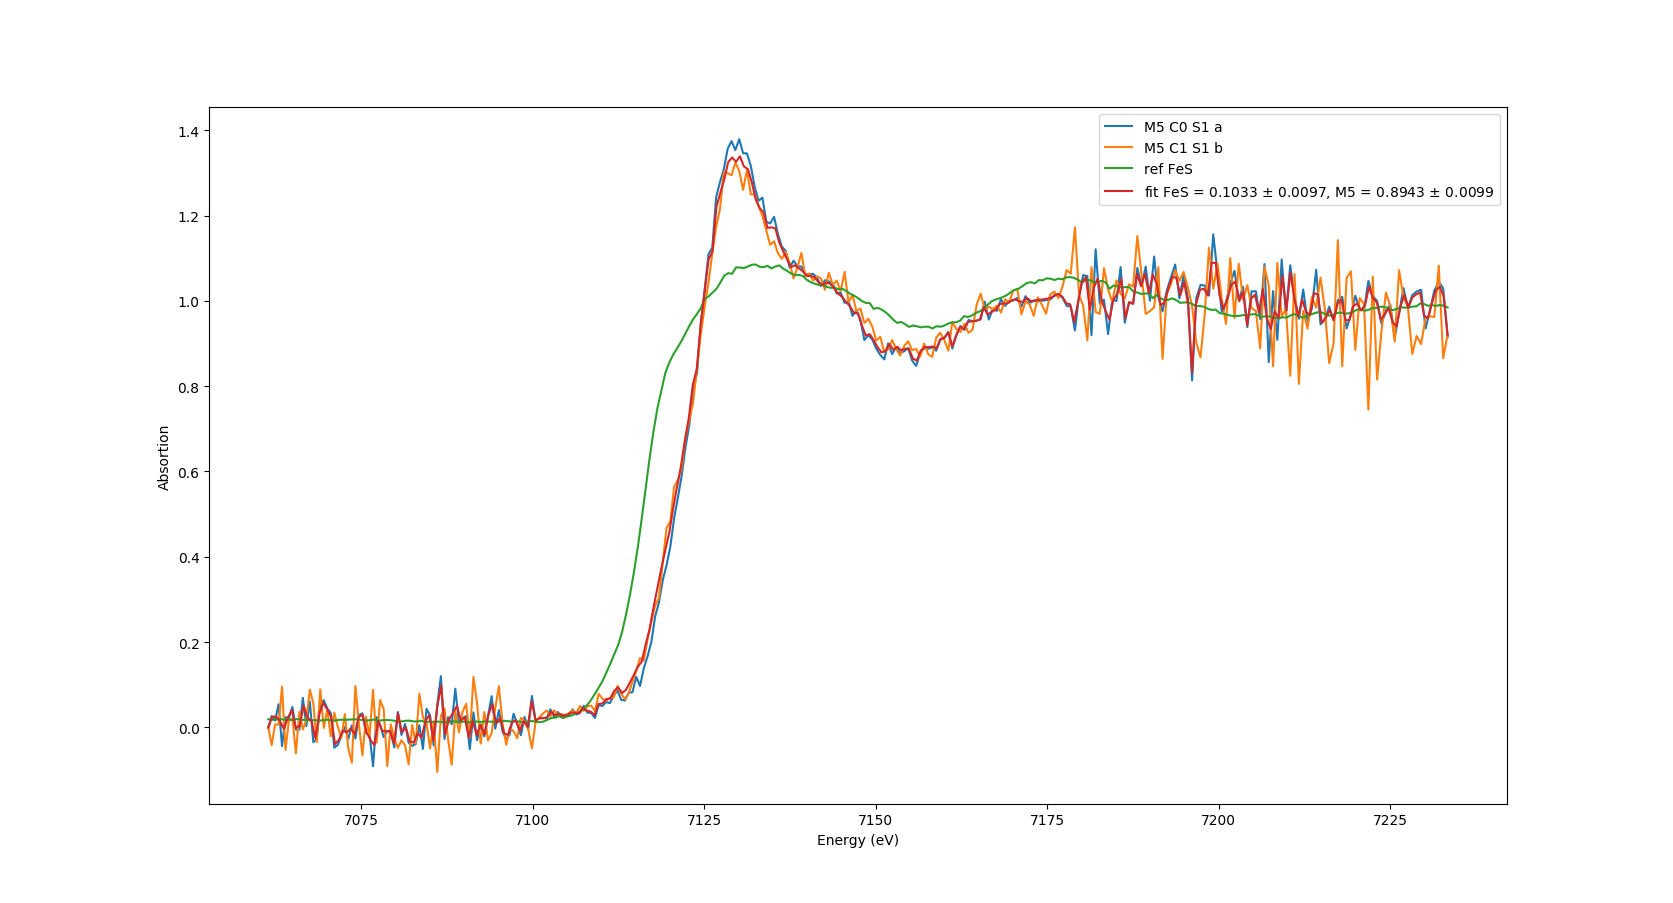
\includegraphics[width=0.9\textwidth]{../Kuvat/Sulfideja/M5_cauchy.png}
%  \caption{M5 soil with added \ch{C} after two months of incubation, compared with \ch{FeS} reference and the case with no added \ch{C}.}
%  \label{fig:M5_C}
%\end{figure}
We also measured the M3 soil, but our co-workers forgot to add the \ch{C}, so there was no change in the chemical state. However this further verifies, that adding organic \ch{C} indeed is needed for \ch{FeS} production to take place. The measurement result of M3 soil is found on appendices in figure \ref{fig:M3_C}.

%\begin{figure}[!htb]
%  \centering
%    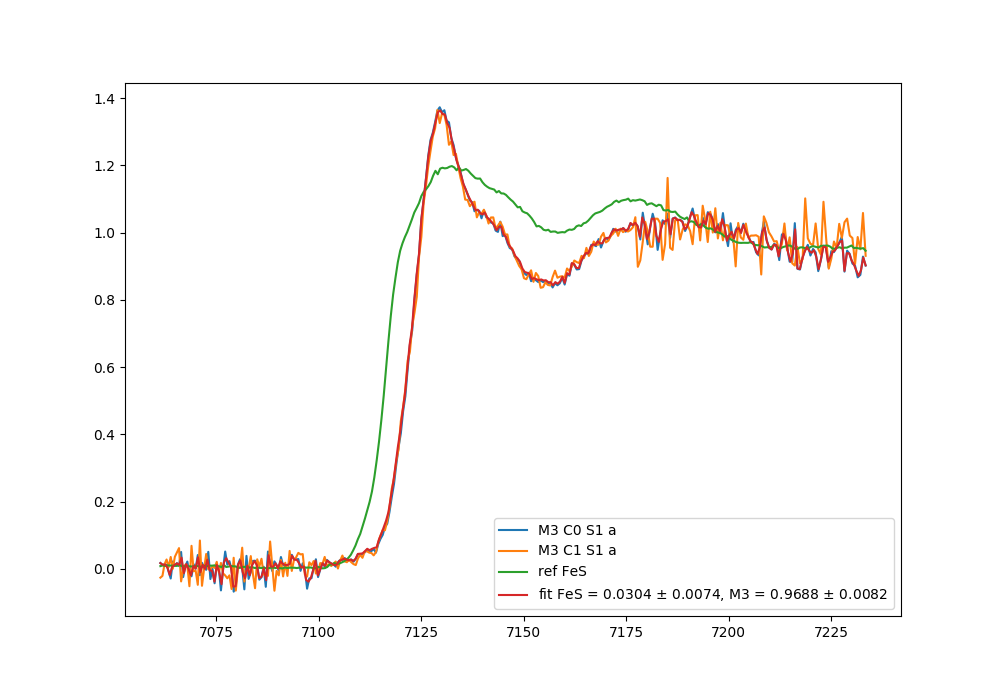
\includegraphics[width=0.8\textwidth]{../Kuvat/Sulfideja/M3_alustava.png}
%  \caption{M3 soil, where the \ch{C} was not added. There is little to non change in the chemical state.}
%  \label{fig:M3_C}
%\end{figure}

The samples were compared with the samples with no added \ch{C} and a reference \ch{FeS} sample. Based on these we performed a least squares fit and also taking into account outlier point. As a result we noticed that sulphides had been formed as follows; M1: $\ch{FeS}=0.19\pm0.01$, M2: $\ch{FeS}=0.16\pm0.02$, M4:$\ch{FeS}=0.19\pm0.02$, M5:$\ch{FeS}=0.10\pm0.01$. 

\subsubsection{Samples with no added Sulfates}
The last set of measurements contained the anaerobic wet samples of M1 and M5 soils, where there was no \ch{S} in the samples. There were two different sets of these samples, one with no added \ch{C} and the other with \ch{C}. Results for M5 soil are shown in figures  \ref{fig:M5_C0S0} and \ref{fig:M5_C1S0}. The M1 soil measurements can be found from appendices in figures \ref{fig:M1_C0S0} and \ref{fig:M1_C1S0}.

%\begin{figure}[h!]
%  \centering
%    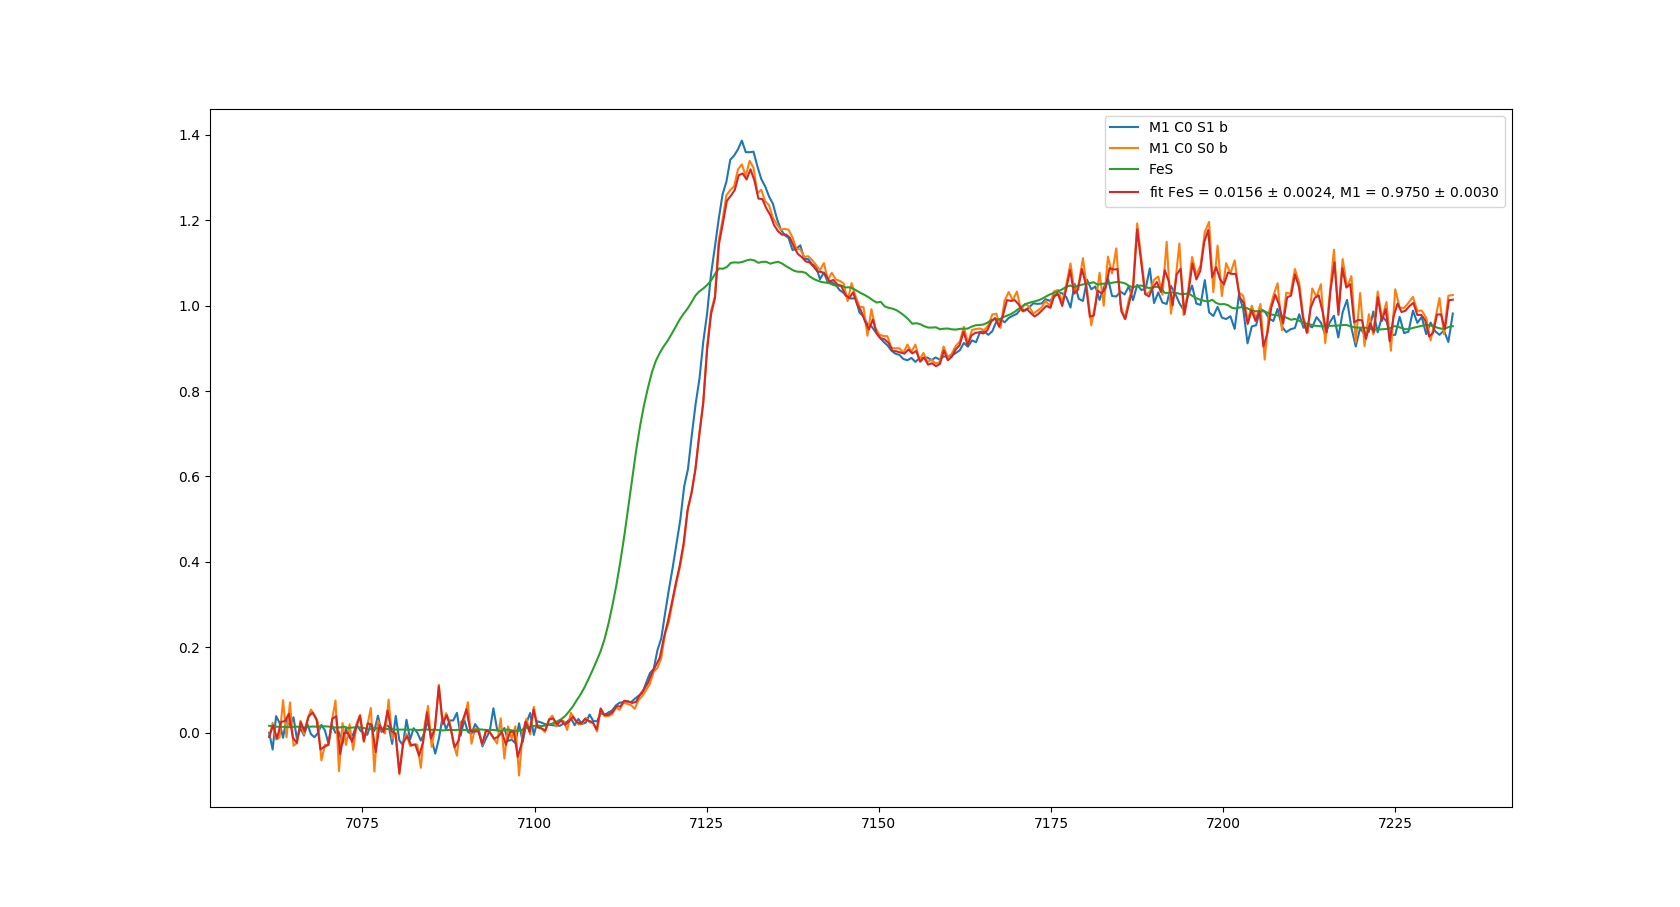
\includegraphics[width=0.9\textwidth]{../Kuvat/Sulfideja/M1C0S0b.png}
%  \caption{M1 soil with no \ch{C} and no \ch{S} after two months of incubation, compared with \ch{FeS} reference and the case with no added \ch{C}.}
%  \label{fig:M1_C0S0}
%\end{figure}

\begin{figure}[h!]
  \centering
    \centerline{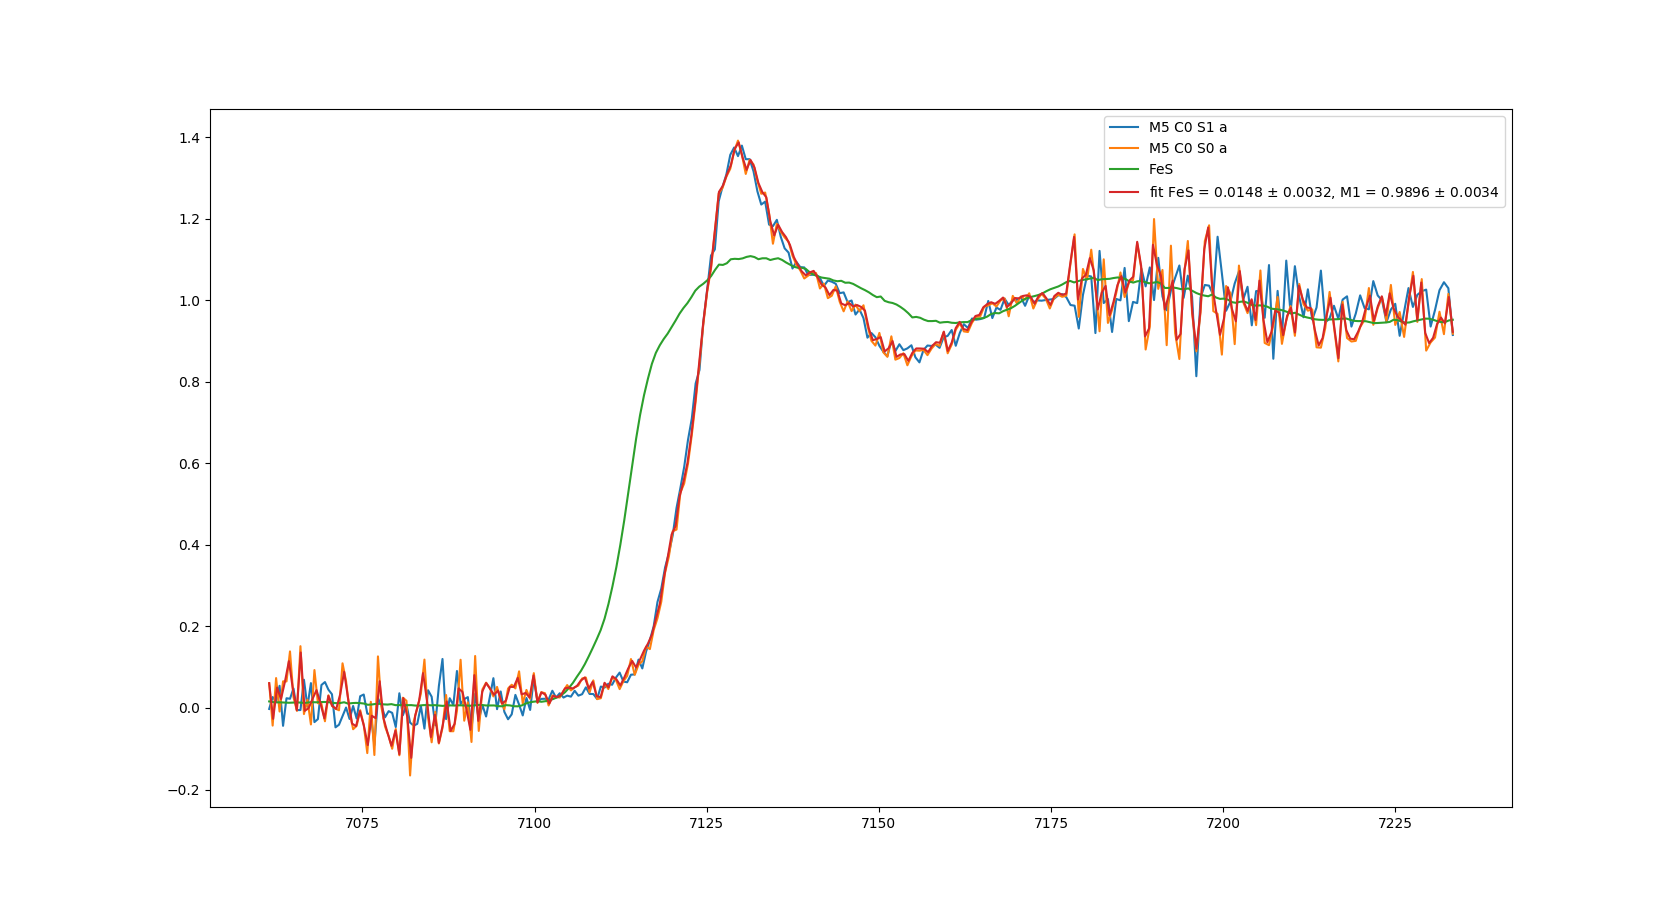
\includegraphics[width=1.3\textwidth]{../Kuvat/Sulfideja/M5C0S1a.png}}
  \caption{M5 soil with no \ch{C} and no \ch{S} after two months of incubation, compared with \ch{FeS} reference and the case with no added \ch{C}.}
  \label{fig:M5_C0S0}
\end{figure}

%\begin{figure}[h!]
%  \centering
%    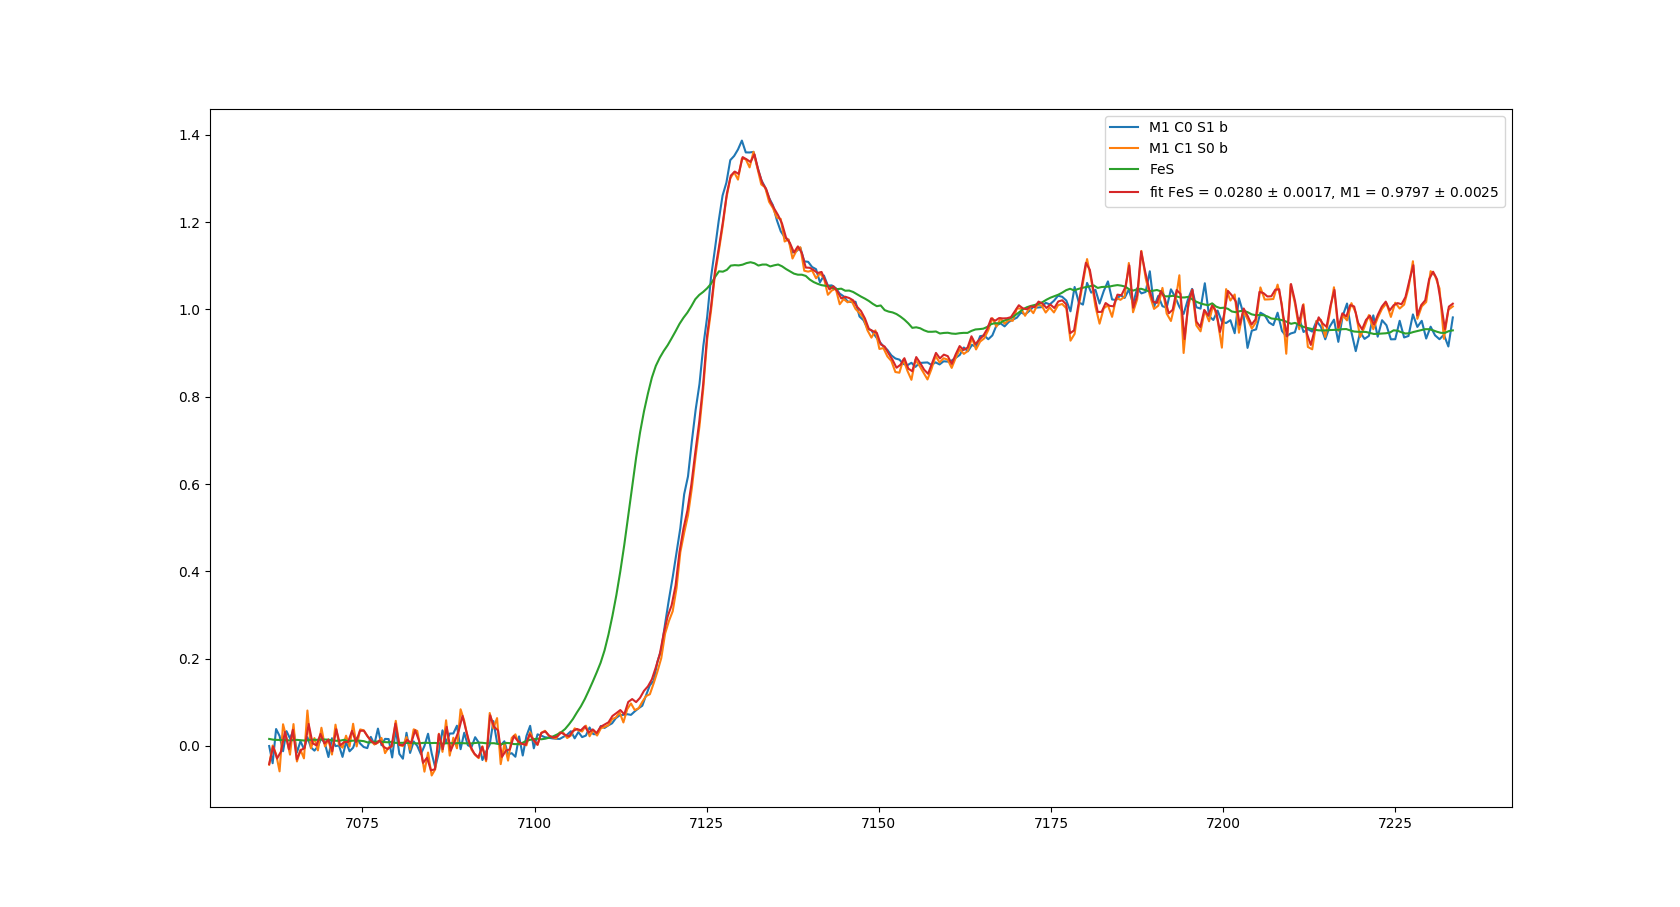
\includegraphics[width=0.9\textwidth]{../Kuvat/Sulfideja/M1C1S0b.png}
%  \caption{M1 soil with the added \ch{C} and no \ch{S} after two months of incubation, compared with \ch{FeS} reference and the case with no added \ch{C}.}
%  \label{fig:M1_C1S0}
%\end{figure}

\begin{figure}[h!]
  \centering
    \centerline{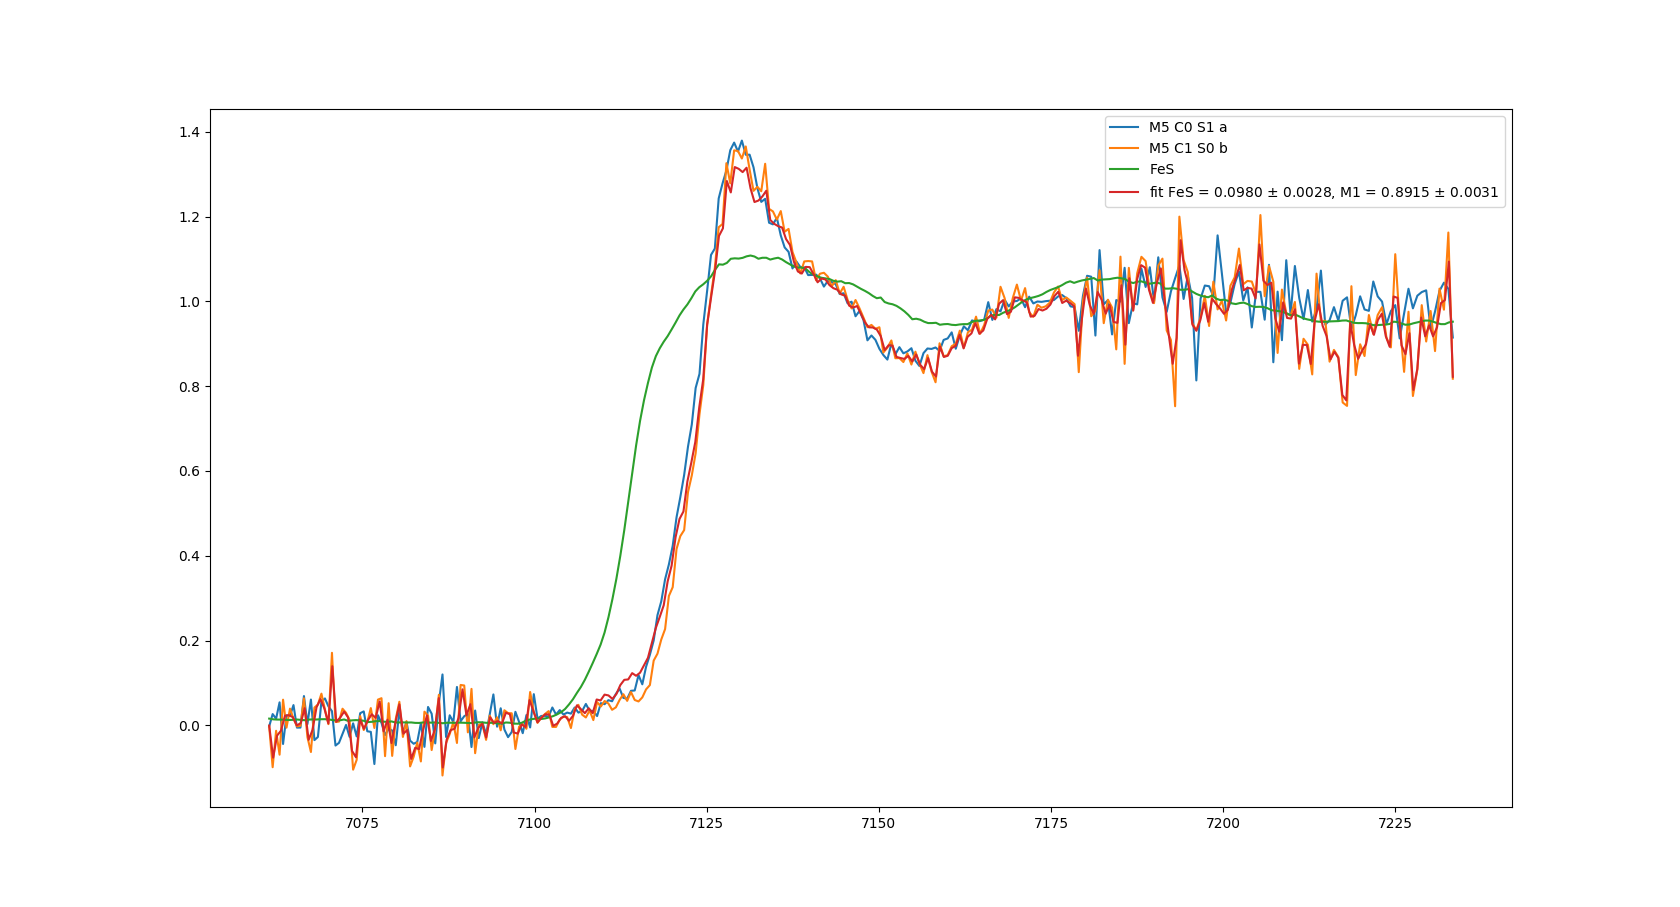
\includegraphics[width=1.3\textwidth]{../Kuvat/Sulfideja/M5C1S0b.png}}
  \caption{M5 soil with the added \ch{C} and no \ch{S} after two months of incubation, compared with \ch{FeS} reference and the case with no added \ch{C}.}
  \label{fig:M5_C1S0}
\end{figure}
Now when there was no \ch{S} in the systems, we saw decreased sulfite levels compared to the samples with the added \ch{S}. For M1C0S0b sample we noted that the sample with added \ch{S} had $1.6\%\pm0.2\%$ more \ch{FeS}. M5C0S1a had $1.5\%\pm0.3\%$ more \ch{FeS} than M5C0S0a, M1C0S1b had $2.8\%\pm0.2\%$ more \ch{FeS} than M1C1S0b, and lastly M5C0S1a had $9.8\%\pm0.3\%$ more \ch{FeS} than M5C1S0b. It seem that some \ch{SO4} reduction takes place, if there is \ch{S} in the system, even without the added \ch{C}. 

\subsection{Chemical Change in Soils after Different Treatments}
With these results we can now form an understanding of the chemical path of \ch{Fe} in our samples. At the beginning the we noticed that \ch{Fe} in our soils were mostly present as \ch{Fe}(III) hydroxides, and shortly after the start of incubations, the chemical state remained the same. After two months of incubation we started to see changes in the chemical state. In case of C0S1 samples we noticed an altered chemical state in comparison with dry samples. We were unfortunately unable to find a matching reference sample for comparison. However we were able notice increased \ch{FeS} production when compared to C0S0 and C1S0 samples. We then compared C1S1 samples with \ch{FeS} reference sample and C0S1 samples. A summary of these measurements results is shown in table \ref{tab:tulos}.
\begin{table}[h!]
\begin{tabular}{|l|l|l|l|}
\hline
Soil & \begin{tabular}[c]{@{}l@{}}C1S1 \ch{FeS} prodution\\ compared with C0S1\end{tabular} & \begin{tabular}[c]{@{}l@{}}C0S1  \ch{FeS} production\\ compared with C0S0\end{tabular} & \begin{tabular}[c]{@{}l@{}}C0S1 \ch{FeS} production\\ compared with C1S0\end{tabular} \\ \hline
M1   & $\ch{FeS}=0.18\pm0.01$                                                                           & $1.6\%\pm0.2\%$                                                                                       & $2.8\%\pm0.2\%$                                                                                       \\ \hline
M2   & $\ch{FeS}=0.16\pm0.01$                                                                            & -                                                                                                       & -                                                                                                      \\ \hline
M3   & C addition failed                                                                                     & -                                                                                                       & -                                                                                                      \\ \hline
M4   & $\ch{FeS}=0.19\pm0.02$                                                                            & -                                                                                                       & -                                                                                                      \\ \hline
M5   & $\ch{FeS}=0.10\pm0.01$                                                                            & $1.48\%\pm0.3\%$                                                                                       & $9.8\%\pm0.3\%$                                                                                       \\ \hline
\end{tabular}
\caption{Summary of the measurement results.}
\label{tab:tulos}
\end{table}

Our results raise few important questions. First we notice the amount of \ch{FeS} production in C1S1 samples. They are rather similar, except for the M5 soil. Interestingly M5 soil has the least amount of sulfide production, while being the most fertile soil. M5 soil also has increased \ch{FeS} production when we compared C0S1 sample with C1S0 sample. Unfortunately we didn't produce C1S0 samples from other soils except M1 soils, since this experiment was more of a pre-experiment before a larger one, so we cannot verify if there is a relation between the result of M5 soil. However this raises possibility for further studies on how the \ch{C} present in soil itself affects \ch{FeS} production and \ch{Fe} oxides ability to bind \ch{P}. 

Our soils were ordered in such a way that the M1 had the highest amount of \ch{Fe} oxides at the beginning of the experiment and other samples were in downward order in terms of the amount of \ch{Fe} oxides. With this in mind we cannot draw any clear conclusion about the amount of \ch{Fe} oxides present in soil and the percentage of \ch{FeS} production after incubation, since the order of \ch{FeS} production does not correlate with the numbering of the samples. We can however state that since we have \ch{FeS} production, the \ch{Fe} in these sulfides is no longer able to bind \ch{P}.  



\chapter{Conclusion}\label{conc}
In this work we developed a method to measure sediment samples in various conditions. We were able to measure and get meaningful results from our samples, and the method is easy to apply into other measurements as well.

%results
In our measurements we were able to verify that \ch{Fe} in our five different dry soils were mainly in \ch{Fe}(III) hydroxides. Twenty four hours after the soils were exposed to the water, the chemical state remained the same, an observation that is in agreement with our hypothesis  that no rapid mineralogical changes occur in aerobic conditions \cite{SoilErosion}. After two months of anaerobic incubation we started to see changes. The chemical state of the samples with no added \ch{C} was slightly altered, however we were not able to verify which \ch{Fe} mineral was formed, since none of our reference samples matched this result. Based on our simulations and literature, we expect this new mineral to be either vivianite, or some other unoxidised \ch{Fe} mineral. In case of anaerobic samples with the added \ch{C}, we noticed the production of \ch{FeS}. In our samples the production of \ch{FeS} was between $10-20\%$, which indicates, that \ch{P} bound in \ch{Fe}(III) oxides was released to the water. With no \ch{S} in the system, we saw smaller \ch{FeS} levels, between $1.5-10\%$ compared to the samples, with the added \ch{S} but no \ch{C}. This means that small amount of \ch{SO4} reduction takes place even without the added \ch{C}.  

%uncertainties
%We noticed few uncertainties affecting our measurements. The gel we produced had to have right water/soil concentration. In the first sampling we took rather small amounts of water or soil in some cases, which made the sample preparation more difficult than needed. We noticed that when we had very little soil, the spectra was affected, possibly due to radiation damage, or \ch{Fe203} present in water. In future studies we advise to take this into account when performing the sampling from incubations. The sample environment was also rather heavy for our small stepper motor, and the movements were sometimes a bit sluggish. This can be taken into account by lightening the sample environment by removing excess aluminium. 
The largest uncertainty arises from the fact that we cannot be sure if our reference samples truly represent the new chemical species in the final state, which can cause systematic error in our results. In order to take this into account in further studies we recommend to try a combination of several reference samples, such us \ch{FeS} and \ch{FeS2}. Even though our curve fits relatively well with the measurement, this way could allow even better results. Other possible sources of error are the algae production in our samples, and exposure of anaerobic samples to oxygen during sample preparation or measurement. During sample preparation we heated up the water and agar mix, which at some point started water stared to vaporize and form bubbles. If some of these bubbles were present after cooling the sample, they might have caused systematic error in case of the wet samples. Also the gain size of samples is easy to control when preparing the dry samples, but for wet samples is recommended to ensure that the grain size is small enough, before starting the incubation.

%discussing the results
The main benefit of our results are not necessarily the results, but the questions, which were left open and raised. What is the unidentified new component in our C0S1 samples? What is the relation of the number of \ch{Fe} oxides and \ch{C} present in soil? What is the relation between available \ch{Fe} oxides and \ch{FeS} production? However, since we noticed \ch{FeS} production, it is likely that \ch{P} is released from the sediment and thus available for polluting the water. 
%future work

The method opens up possibilities for future work. With a larger amount of samples and with various water types one can form a more accurate picture of the sediment processes. The measurements could also be complimented with \ch{Mn} XANES studies and possibly even with \ch{P} studies on a synchrotron. With these additions to our result one could form a model of the sediment processes to be taken into account when planning the guidelines for erosion control measures around the Baltic sea and other water bodies vulnerable to eutrophication.

Another important measurement to complement our results would be to measure vivianite and other \ch{Fe} minerals, such as \ch{FeS2}. In order to measure the vivianite, reference material  probably has to be self made chemically in an anaerobic environment to avoid oxidation. Also other \ch{Fe} minerals might be sensitive to oxidation, and it is possible that those are also present in our measurements.

All in all we were able to verify the production of sulphides under anoxic environment in our samples. This is in line with the model discussed in section 2.4. The sediment processes are currently not taken into account in erosion and phosphorus release guidelines. With further studies a more detailed model of sediment processes can be produced to be taken into account in the guidelines.


\bibliographystyle{unsrt}
\bibliography{luettelo}

\begin{appendices}
\chapter{Wet Samples After 24 hours}


\begin{figure}[h!]
  \centering
     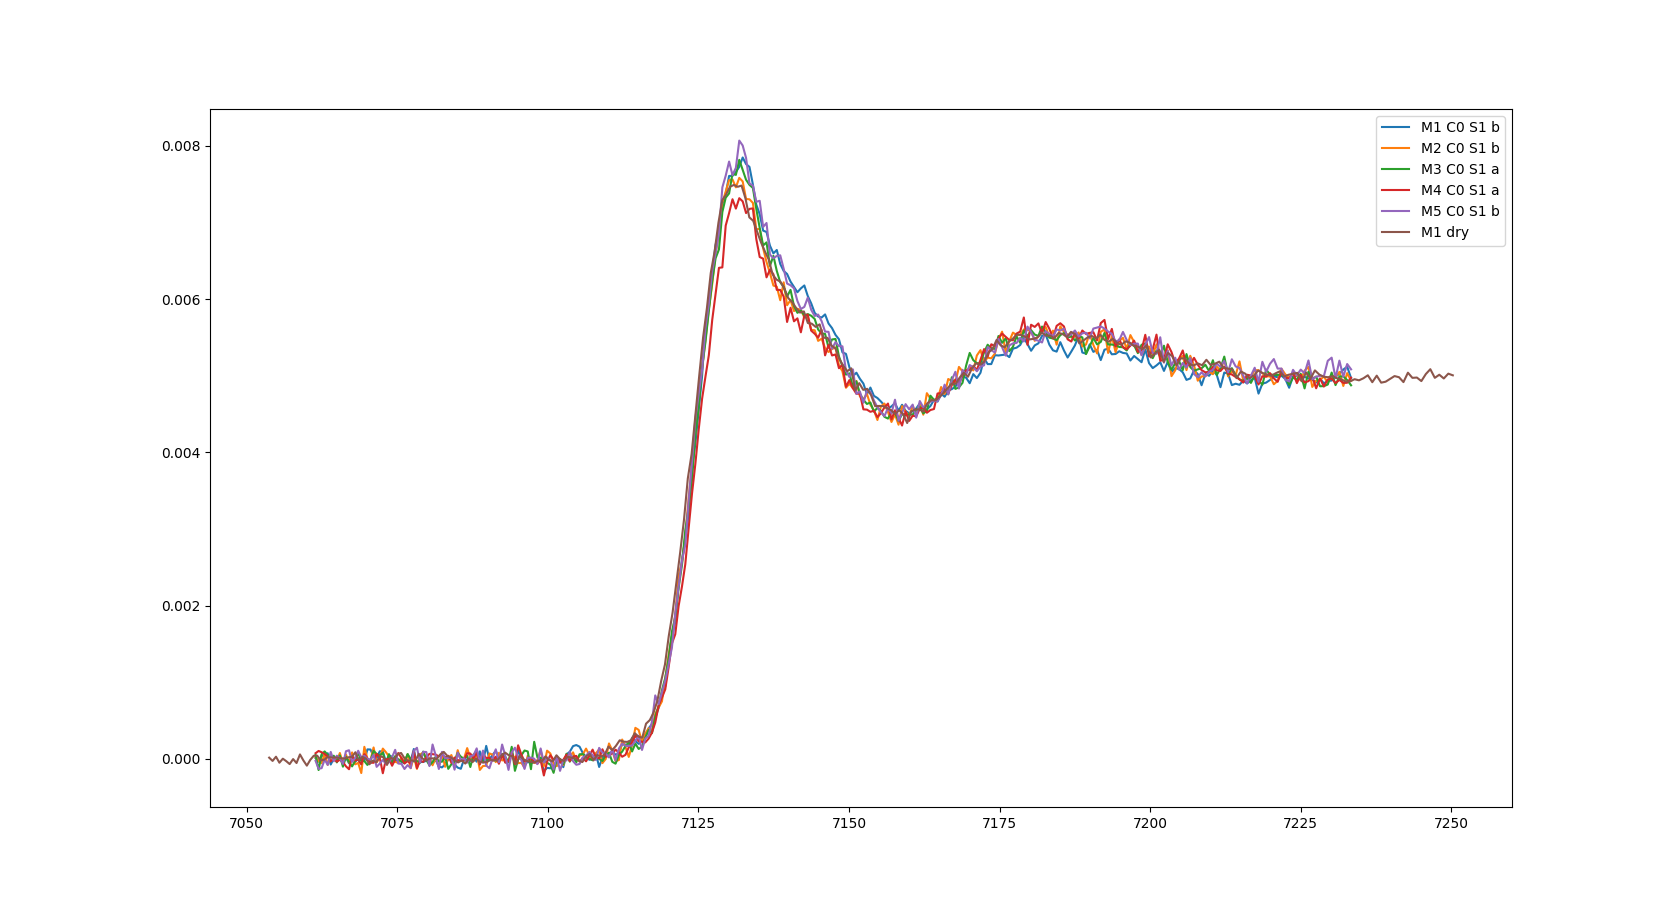
\includegraphics[width=\textwidth]{../Kuvat/Sulfideja/wet_noC.png}
  \caption{The spectra of wet samples with no added \ch{C} after 24 hours of incubation.}
  \label{fig:wetsoilC}
\end{figure}

\begin{figure}[h!]
  \centering
     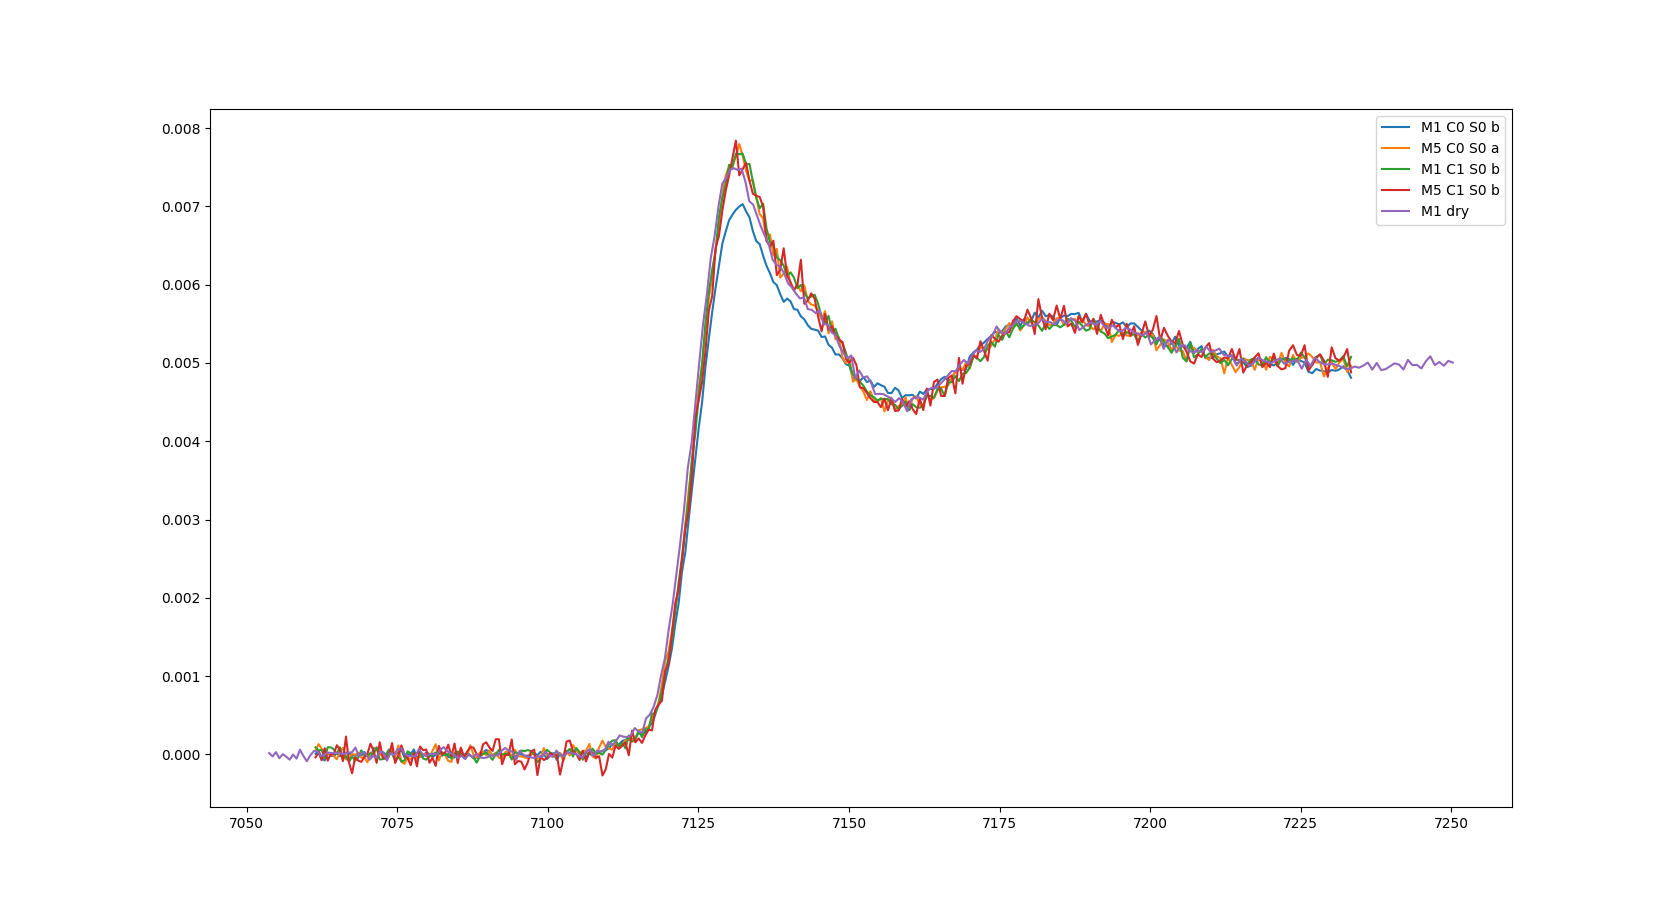
\includegraphics[width=\textwidth]{../Kuvat/Sulfideja/wetOthers.png}
  \caption{The spectra of wet samples with no added sulphides.}
  \label{fig:wetsoil_others}
\end{figure}
\chapter{Anaerobic Samples With No Added Carbon}

\begin{figure}[h!]
  \centering
    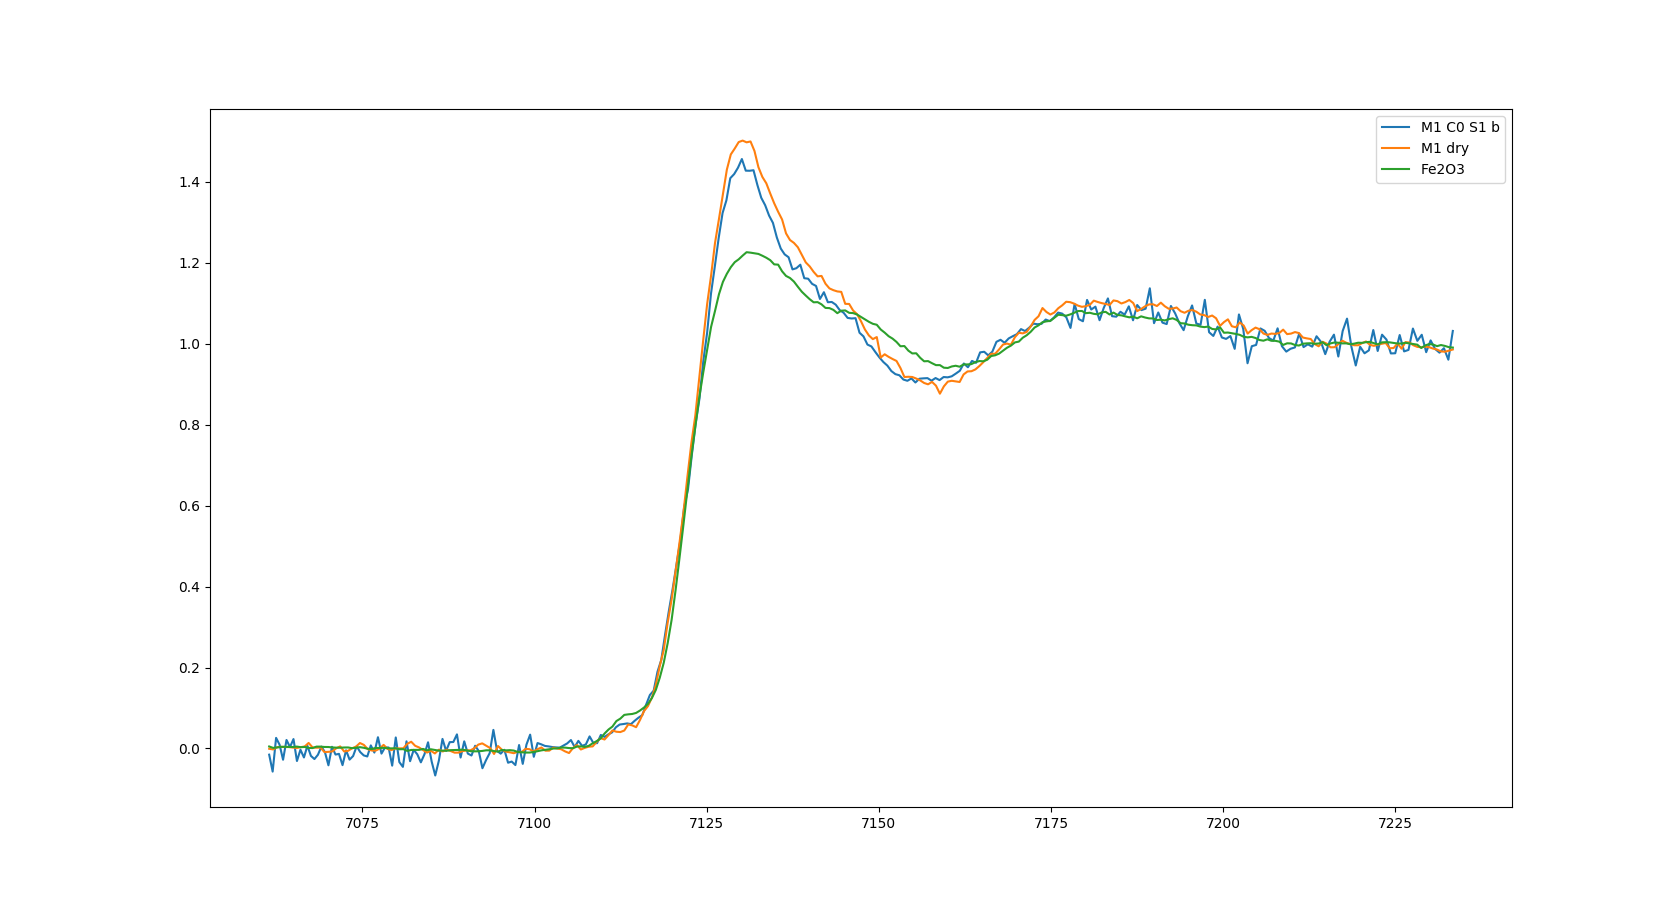
\includegraphics[width=0.9\textwidth]{../Kuvat/Sulfideja/M1_Fe2O3.png}
  \caption{M1 soil with no added \ch{C} after two months of incubation. The results are compared to the dry sample and \ch{Fe2O3} reference sample.}
  \label{fig:M1_noC}
\end{figure}

\begin{figure}[h!]
  \centering
    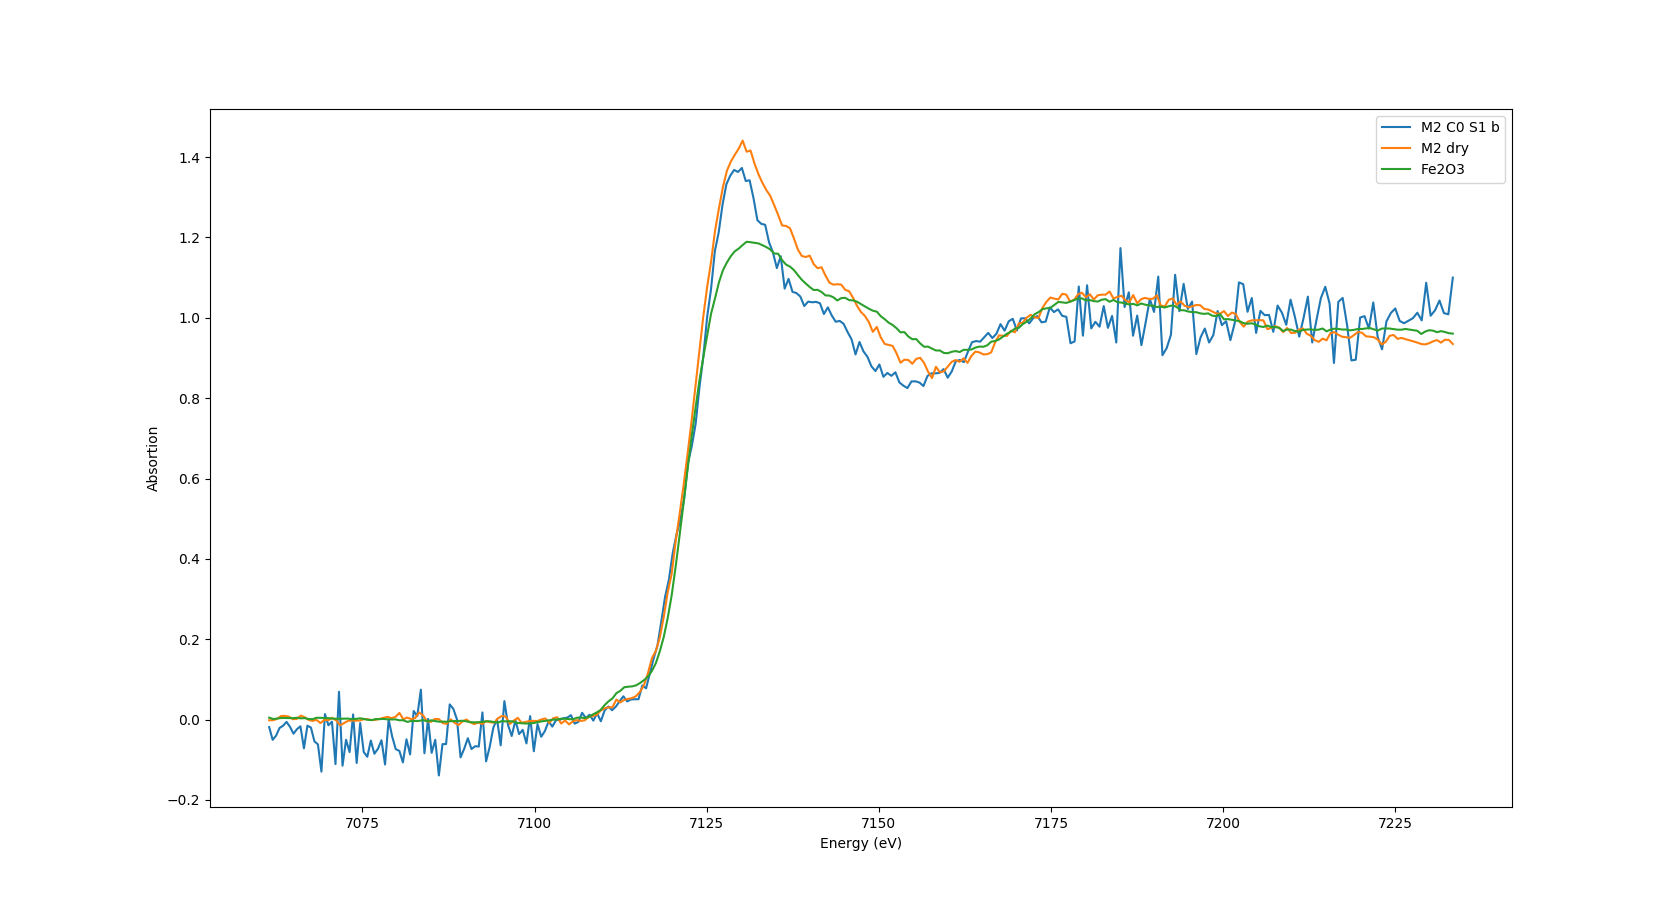
\includegraphics[width=0.9\textwidth]{../Kuvat/Sulfideja/M2_Fe2O3.png}
  \caption{M2 soil with no added \ch{C} after two months of incubation. The results are compared to the dry sample and \ch{Fe2O3} reference sample.}
  \label{fig:M2_noC}
\end{figure}

\begin{figure}[h!]
  \centering
    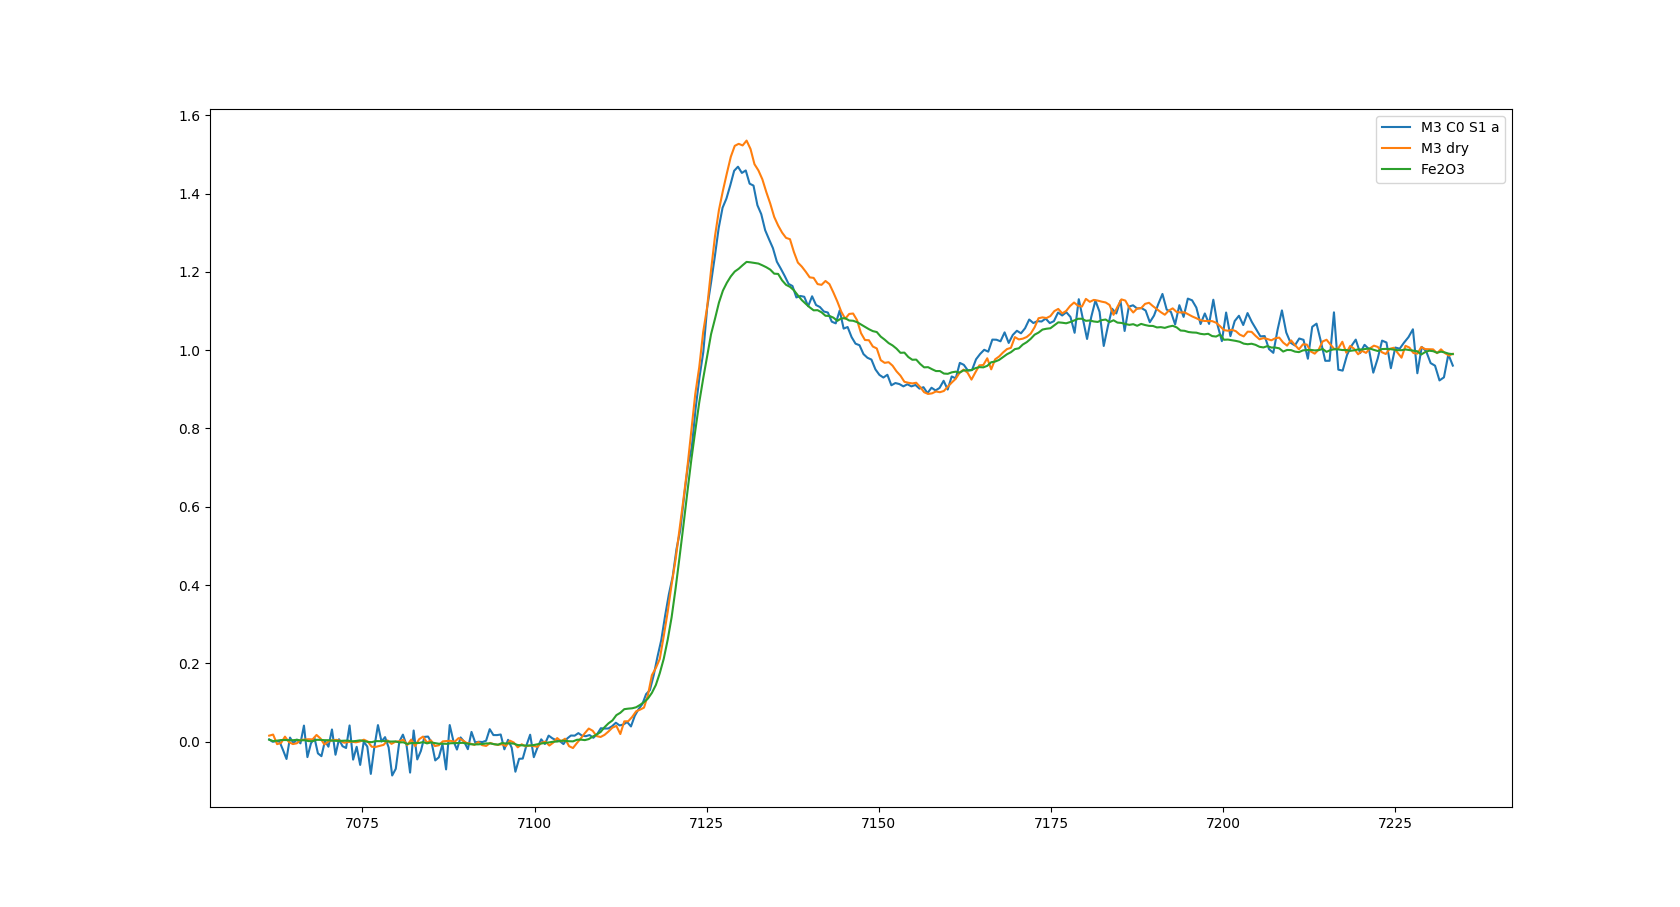
\includegraphics[width=0.9\textwidth]{../Kuvat/Sulfideja/M3_Fe2O3.png}
  \caption{M3 soil with no added \ch{C} after two months of incubation. The results are compared to the dry sample and \ch{Fe2O3} reference sample.}
  \label{fig:M3_noC}
\end{figure}

%\begin{figure}[h!]
%  \centering
%    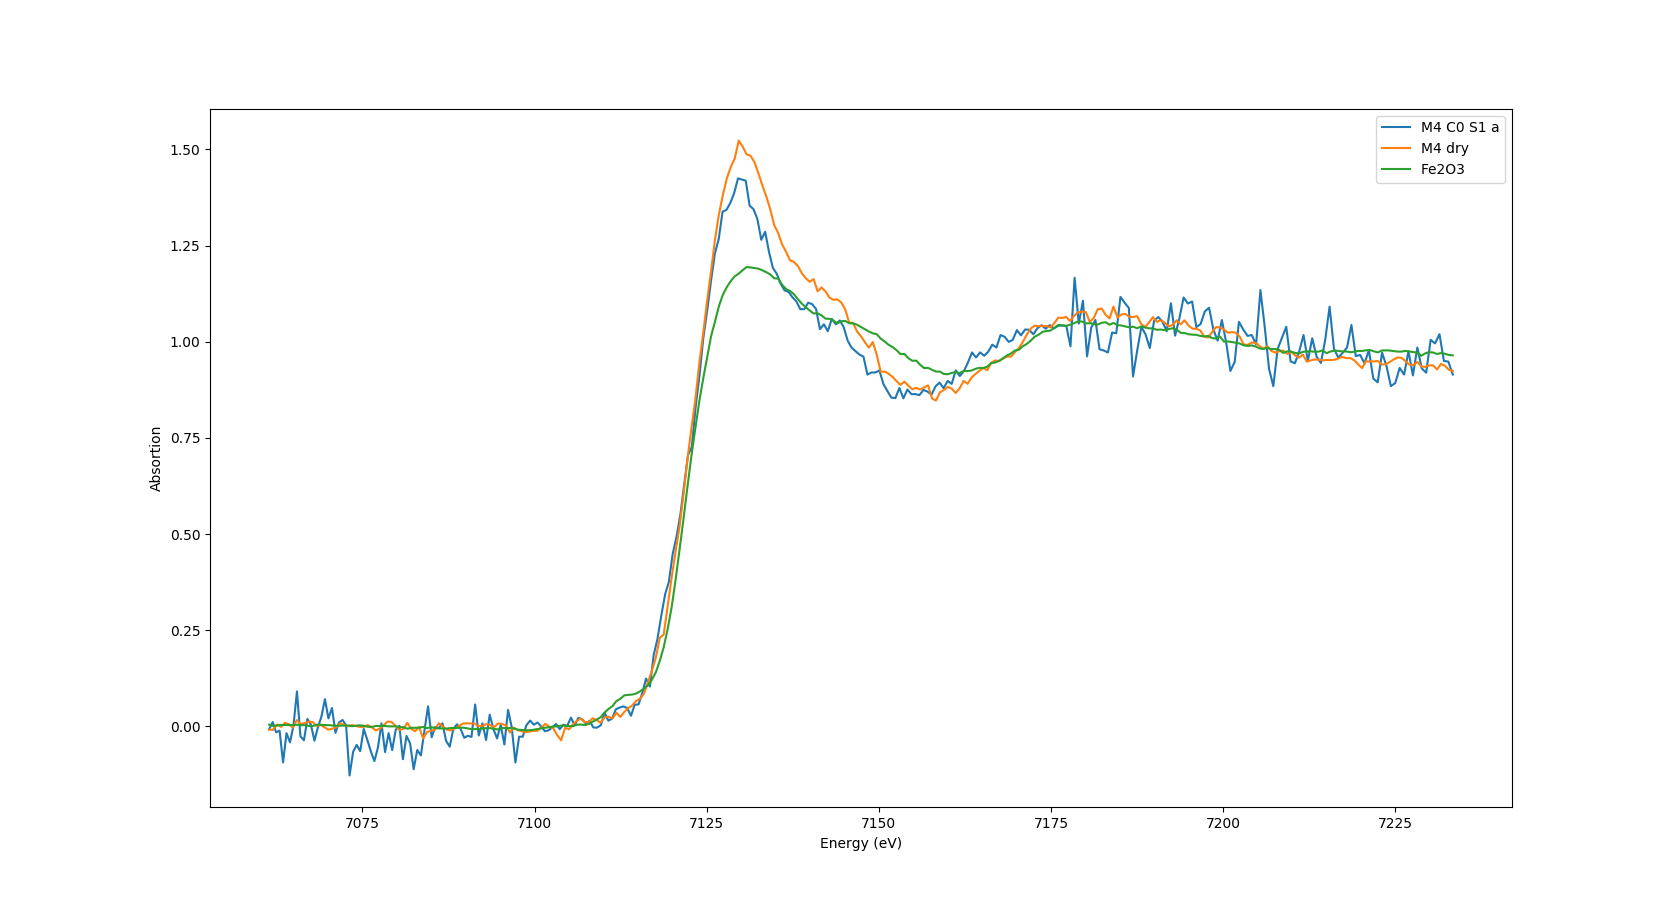
\includegraphics[width=0.9\textwidth]{../Kuvat/Sulfideja/M4_Fe2O3.png}
%  \caption{M4 soil with no added \ch{C} after two months of incubation. The results are compared to the dry sample and \ch{Fe2O3} reference sample.}
%  \label{fig:M4_noC}
%\end{figure}

\begin{figure}[h!]
  \centering
    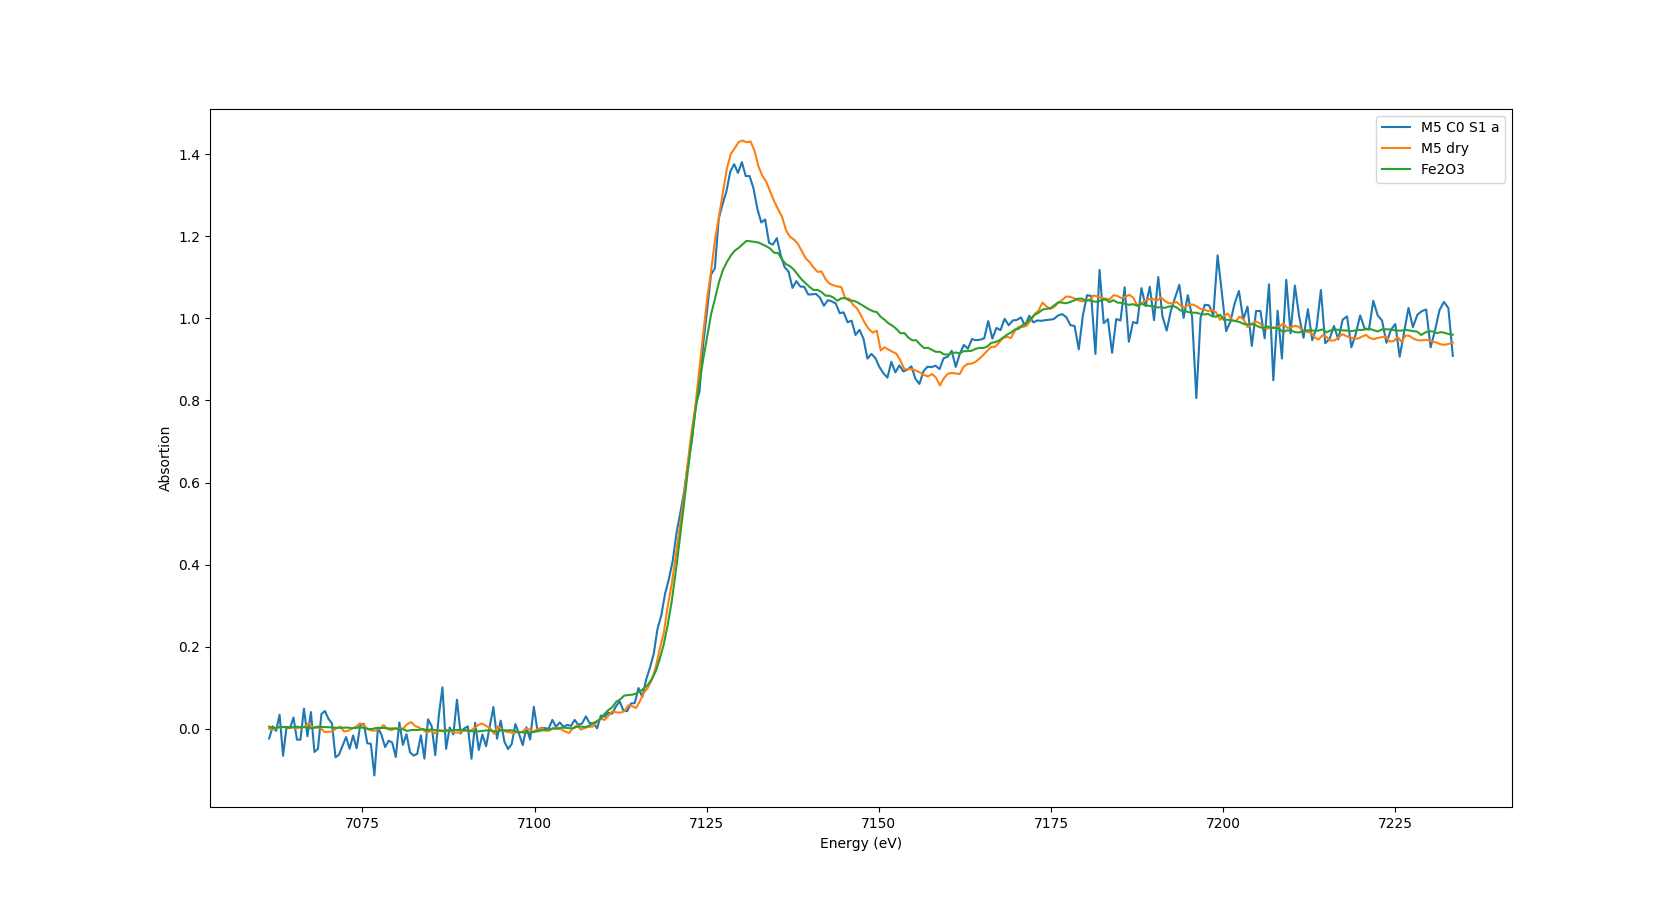
\includegraphics[width=0.9\textwidth]{../Kuvat/Sulfideja/M5_noC.png}
  \caption{M5 soil with no added \ch{C} after two months of incubation. The results are compared to the dry sample and \ch{Fe2O3} reference sample.}
  \label{fig:M5_noC}
\end{figure}

\chapter{Anaerobic Samples With Added Carbon}

\begin{figure}[!htb]
  \centering
    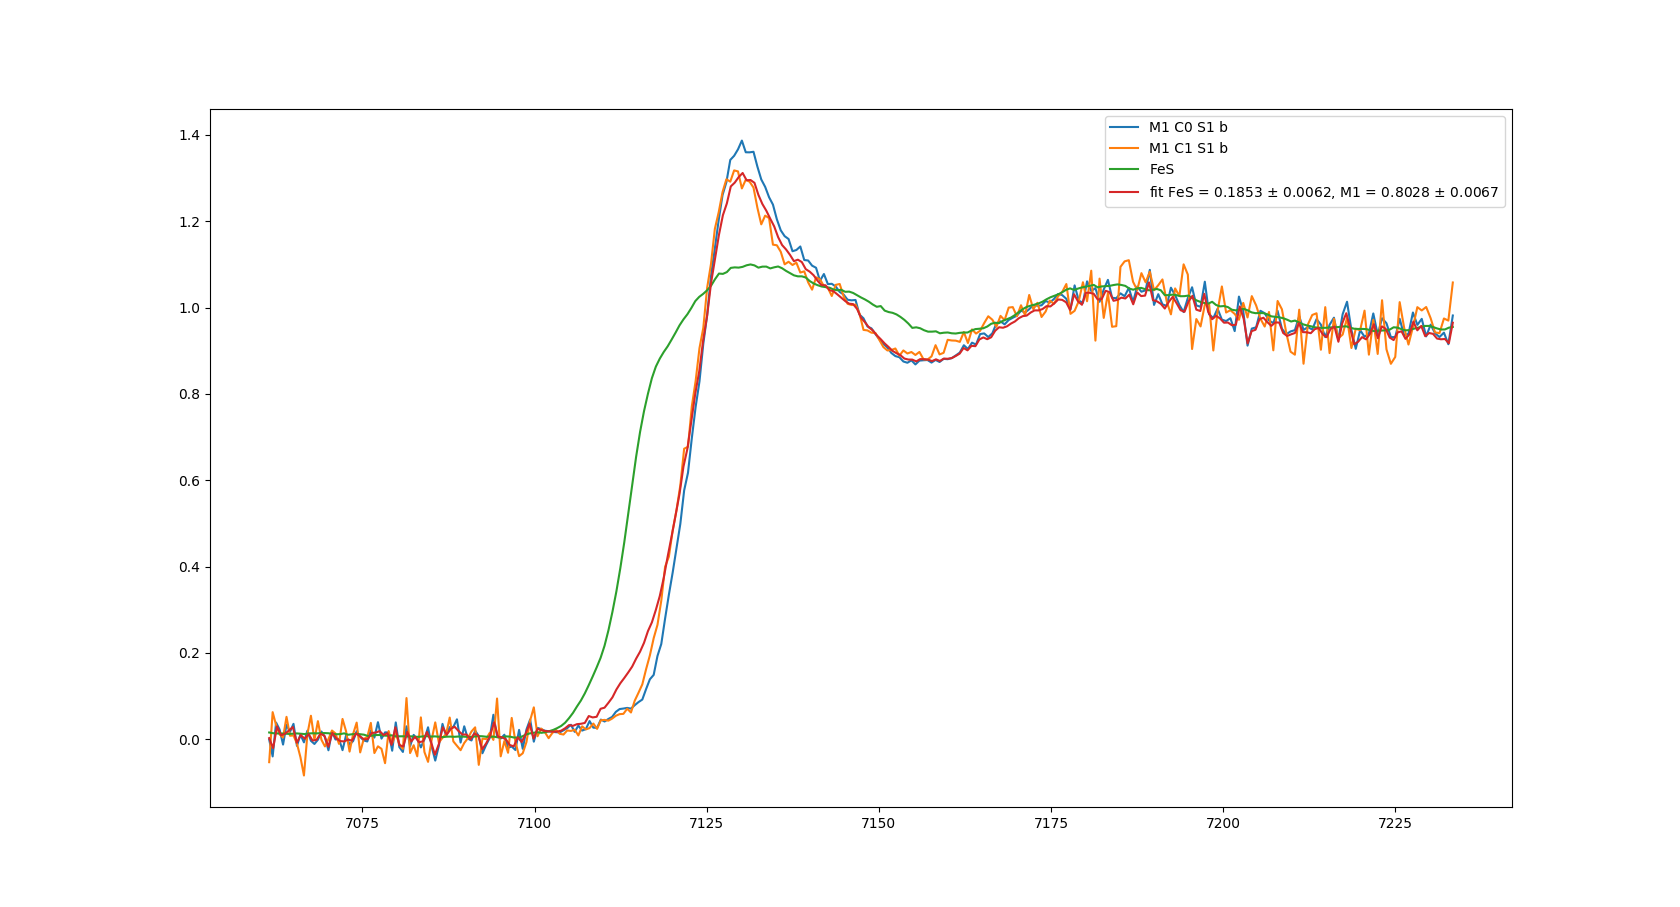
\includegraphics[width=0.9\textwidth]{../Kuvat/Sulfideja/M1_cauchy.png}
  \caption{M1 soil with added \ch{C} after two months of incubation, compared with \ch{FeS} reference and the case with no added \ch{C}}
  \label{fig:M1_C}
\end{figure}

\begin{figure}[!htb]
  \centering
    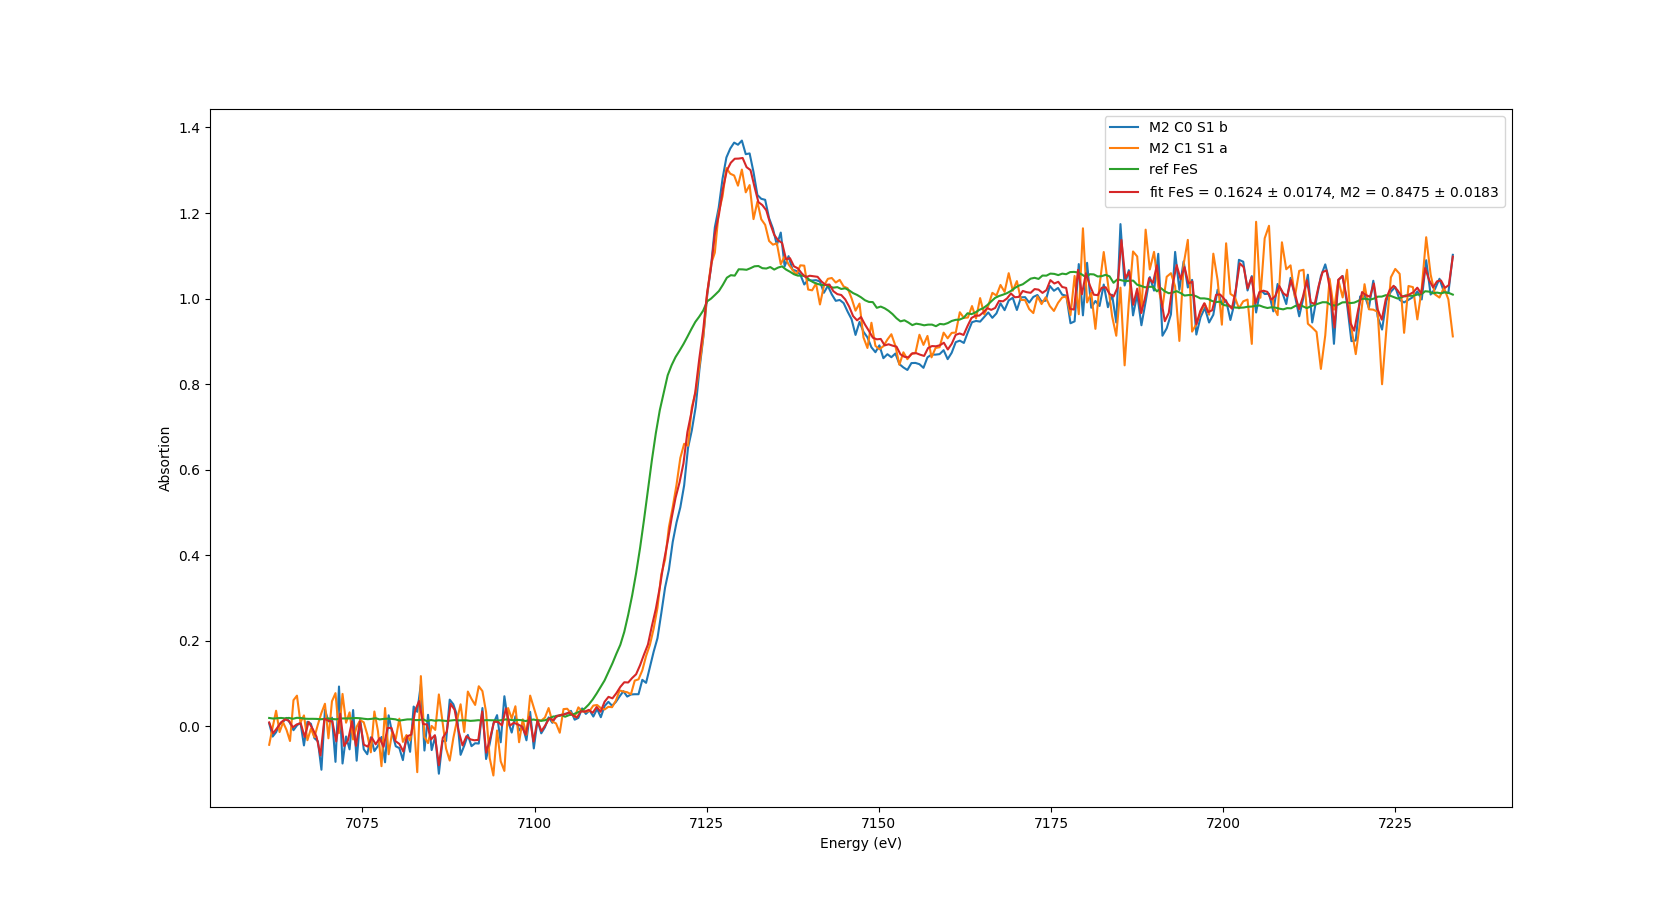
\includegraphics[width=0.9\textwidth]{../Kuvat/Sulfideja/M2_cauchy.png}
  \caption{M2 soil with added \ch{C} after two months of incubation, compared with \ch{FeS} reference and the case with no added \ch{C}.}
  \label{fig:M2_C}
\end{figure}

%\begin{figure}[!htb]
%  \centering
%    \includegraphics[width=0.9\textwidth]{../Kuvat/Sulfideja/M4_cauchy.png}
%  \caption{M4 soil with added \ch{C} after two months of incubation, compared with \ch{FeS} reference and the case with no added \ch{C}.}
%  \label{fig:M4_C}
%\end{figure}

\begin{figure}[!htb]
  \centering
    \includegraphics[width=0.9\textwidth]{../Kuvat/Sulfideja/M5_cauchy.png}
  \caption{M5 soil with added \ch{C} after two months of incubation, compared with \ch{FeS} reference and the case with no added \ch{C}.}
  \label{fig:M5_C}
\end{figure}

\begin{figure}[!htb]
  \centering
    \includegraphics[width=0.8\textwidth]{../Kuvat/Sulfideja/M3_alustava.png}
  \caption{M3 soil, where the \ch{C} was not added. There is little to non change in the chemical state.}
  \label{fig:M3_C}
\end{figure}

\chapter{Anaerobic Samples With No added Sulfates}
\begin{figure}[h!]
  \centering
    \includegraphics[width=0.9\textwidth]{../Kuvat/Sulfideja/M1C0S0b.png}
  \caption{M1 soil with no \ch{C} and no \ch{S} after two months of incubation, compared with \ch{FeS} reference and the case with no added \ch{C}.}
  \label{fig:M1_C0S0}
\end{figure}

\begin{figure}[h!]
  \centering
    \includegraphics[width=0.9\textwidth]{../Kuvat/Sulfideja/M1C1S0b.png}
  \caption{M1 soil with the added \ch{C} and no \ch{S} after two months of incubation, compared with \ch{FeS} reference and the case with no added \ch{C}.}
  \label{fig:M1_C1S0}
\end{figure}

\end{appendices}

\end{document}
